\documentclass[a4paper,twoside,DIV15,BCOR12mm]{scrbook}
\usepackage{ana}
\usepackage{tikz}
\usepackage{wrapfig}

\pdfinfo{
	/Author (Die Mitarbeiter von http://mitschriebwiki.nomeata.de/)
	/Title   (Analysis I)
	/Subject (Analysis I)
	/Keywords (Analysis)
}

\author{Die Mitarbeiter von \url{http://mitschriebwiki.nomeata.de/}}
\title{Analysis I}
\makeindex

\begin{document}
\maketitle

\renewcommand{\thechapter}{\Roman{chapter}}
%\chapter{Inhaltsverzeichnis}
\addcontentsline{toc}{chapter}{Inhaltsverzeichnis}
\tableofcontents

\chapter{Vorwort}

\section{Über dieses Skriptum}
Dies ist ein erweiterter Mitschrieb der Vorlesung \glqq Analysis I\grqq\ von Herrn Schmoeger im
Wintersemester 04/05 an der Universität Karlsruhe (TH). Die Mitschriebe der Vorlesung werden mit
ausdrücklicher Genehmigung von Herrn Schmoeger hier veröffentlicht, Herr Schmoeger ist für den
Inhalt nicht verantwortlich.

\section{Wer}
Gestartet wurde das Projekt von Joachim Breitner. Beteiligt am Mitschrieb sind ausser Joachim
noch Manuel Holtgrewe, Wenzel Jakob, Pascal Maillard und Jonathan Picht.

\section{Wo}
Alle Kapitel inklusive \LaTeX-Quellen können unter \url{http://mitschriebwiki.nomeata.de} abgerufen werden.
Dort ist ein \emph{Wiki} eingerichtet und von Joachim Breitner um die \LaTeX-Funktionen erweitert.
Das heißt, jeder kann Fehler nachbessern und sich an der Entwicklung
beteiligen. Auf Wunsch ist auch ein Zugang über \emph{Subversion} möglich.

\chapter{Eingeführte Begriffe}

\section{Mengen}

Durchschnitt, Vereinigung, Differenz, Leere Menge: $\emptyset$, $M\subseteq N$, $M\subset N$, $a \in M$, $a\notin M$

\section{Funktionen}

$M$,$N$ Mengen, $M,N \ne \emptyset$; $f:\, M\rightarrow N$

\section{Logik}

\begin{itemize}
\item $\Rightarrow$ Implikation
\item $\Leftrightarrow$ Äquivalenz
\item $:=$ per Definition gleich
\item $:\Leftrightarrow$ per Definiton äquivalent
\item $\forall$ Abkürzung für \glqq für jedes\grqq, \glqq für alle\grqq
\item $\exists$ Abkürzung für \glqq es gibt\grqq, \glqq es existiert\grqq
\end{itemize}



\renewcommand{\thechapter}{\arabic{chapter}}
\renewcommand{\chaptername}{§}
\setcounter{chapter}{0}

\chapter{Reelle Zahlen}

Die \begriff{Reellen Zahlen} sind eine Erfindung des menschlichen Geistes, sie haben von Natur aus keine Eigenschaften. Wie Schachfiguren haben sie nur eine Bedeutung im Rahmen der Regeln. Diese Regeln heißen hier Axiome, das sind Forderungen, die wir an etwas stellen, und aus denen wir dann weitere Erkenntnisse erlangen.

Die Grundmenge der Analysis ist $\MdR$, die Menge der reellen Zahlen: Diese Menge führen wir axiomatisch ein, durch die folgenden 15 Axiome.

In $\MdR$ sind zwei Verknüpfungen \glqq +\grqq und \glqq $\cdot$\grqq gegeben, die jedem Paar $a,b \in \MdR$ genau ein $ a+b \in \MdR$ und genau ein $ ab := a \cdot b \in \MdR$ zuordnen.

\indexlabel{Körperaxiome}\begin{axiom}[K"orperaxiome]
\begin{liste}
\item[(A1)] $a+(b+c) = (a+b)+c \ \forall a,b,c \in \MdR$
\item[(A2)] $a(bc) = (ab)c \ \forall a,b,c \in \MdR$
\item[(A3)] $a+b = b+a \ \forall a,b \in \MdR$
\item[(A4)] $ab = ba \ \forall a,b \in \MdR$
\item[(A5)] $\exists 0 \in \MdR: a + 0 = a \ \forall a \in \MdR$
\item[(A6)] $\exists 1 \in \MdR\setminus\{0\}: a \cdot 1 = a \ \forall a \in \MdR$
\item[(A7)] $\forall a \in \MdR\ \exists -a \in \MdR: a + (-a) = 0 $
\item[(A8)] $\forall a \in \MdR \setminus \{0\}\ \exists a^{-1} \in \MdR: a a^{-1} = 1 $
\item[(A9)] $a(b+c) = ab + ac \ \forall a,b,c \in \MdR$
\end{liste}
\end{axiom}

Dabei nennt man \textbf{A1} und \textbf{A2} \begriff{Assoziativgesetze}, \textbf{A3} und \textbf{A4} \begriff{Kommutativgesetze} und \textbf{A9} \begriff{Distributivgesetz}, 

Alle Regeln der Grundrechenarten lassen sich aus \textbf{(A1)} bis \textbf{(A9)} herleiten. diese Regeln seien von nun an bekannt.

\begin{beispiele}
\item \textbf{Behauptung:} Es gibt genau ein $0 \in \MdR$ mit $a+0 = a \ \forall a\in \MdR$.

\textbf{Beweis:} Die Existenz folgt direkt aus \textbf{(A5)}. Der Beweis der Eindeutigkeit: Es sei $\tilde 0 \in \MdR$ mit $a+\tilde 0 = a \ \forall a \in \MdR$. Daraus folgt $0 + \tilde 0 = 0 \Rightarrow 0 = 0 + \tilde 0 = \tilde 0 + 0 = \tilde 0$, also $0 = \tilde 0$. \textit{(Aufgabe: Beweise die Eindeutigkeit von 1, $-a$, ...)}

\item \textbf{Behauptung:} $a \cdot 0 = 0 \ \forall a \in \MdR$

\textbf{Beweis:} Sei $a\in\MdR$ und $b := a \cdot 0$. Dann $b = a(0+0) = a \cdot 0 + a \cdot 0 = b$. Aus \textbf{(A7)} folgt dann $0 = b + (-b) = (b+b)+(-b) = b + (b+ (-b)) = b + 0  =b$.

\item

\textbf{Behauptung:} Aus $ab= 0$ folgt $a = 0$ oder $b=0$. \textit{Beweis zur Übung}

\end{beispiele}

\begin{schreibweisen}
Für $a,b \in\MdR: a - b := a+ (-b)$; ist $b \neq 0: \frac{a}{b} := ab^{-1}$.
\end{schreibweisen}

\indexlabel{Anordnungsaxiome}\begin{axiom}[Anordnungsaxiome]
In \MdR\ ist eine Relation \glqq$\le$\grqq\ gegeben. Es sollen gelten:
\begin{liste}
\item[(A10)] für $a,b\in\MdR$ gilt $a\le b$ oder $b \le a$.
\item[(A11)] aus $a \le b$ und $b \le a $ folgt $a = b$.
\item[(A12)] aus $a \le b$ und $b \le c $ folgt $a \le c$.
\item[(A13)] aus $a \le b$ und $c \in \MdR$ folgt $a+c \le b+c$.
\item[(A14)] aus $a \le b$ und $0 \le c$ folgt $ac \le bc$.
\end{liste}
\end{axiom}

\textbf{Alle} Regeln für Ungleichungen lassen sich aus \textbf{(A1)} bis \textbf{(A14)} herleiten. Diese Regeln seinen von nun an bekannt.

\begin{schreibweisen}
\begin{liste}
\item $a < b :\Leftrightarrow a \le b $ und $a \ne b$
\item $a > b :\Leftrightarrow b < a$
\item $a \ge b :\Leftrightarrow b \le a$
\end{liste}
\end{schreibweisen}

\begin{definition}[Betrag]
Für $a \in \MdR$ heißt $ |a| := 
\begin{cases}
 a & \mbox{falls } a \ge 0 \\
-a & \mbox{falls } a < 0
\end{cases} $. 

$|a|$ wird der \begriff{Betrag} von a genannt und entspricht dem \glqq Abstand\grqq\ von $a$ und $0$. $|a-b|$ entspricht dem \glqq Abstand\grqq\ von $a$ und $b$.
\end{definition}

\indexlabel{Betragssätze}\begin{satz}[Betragssätze]
\begin{liste}
\item $|a| \ge 0 \ \forall a \in \MdR; |a|= 0 \Leftrightarrow a = 0$
\item $|a-b| = |b-a| \ \forall a,b \in \MdR$
\item $|ab|  = |a| \cdot |b| \ \forall a,b, \in \MdR$
\item $\pm a \le |a|$
\item $|a+b| \le |a|+|b| \ \forall a,b \in \MdR$
\item $||a| - |b|| \le |a - b| \ \forall a,b \in \MdR$
\end{liste}
\end{satz}

\begin{beweise}
\setcounter{enumi}{4}
\item Fall 1: $a+b \ge 0 \Leftrightarrow |a+b| = a+b \le |a| + |b|$ \\
Fall 2: $a+b  <  0 \Leftrightarrow |a+b| = -(a+b) = - a + (-b) \le |a| + |b|$ \\
\item $|a| = |(a-b) + b| \le |a-b| + |b| \Rightarrow |a| - |b| \le |a-b|$, analog $|b|-|a| \le |b-a| = |a-b|$.
\end{beweise}

\indexlabel{Intervall}\begin{definition}[Intervall]
Seien $a,b \in \MdR$, $a<b$:

\begin{liste}
\item $(a,b) := \{ x \in \MdR: a < x < b\} $: \begriff{offenes Intervall}
\item $[a,b] := \{ x \in \MdR: a \le x \le b\} $: \begriff{abgeschlossenes Intervall}
\item $(a,b] := \{ x \in \MdR: a < x \le b\} $: \begriff{halboffenes Intervall}
\item $[a, \infty) := \{ x \in \MdR: a \le x \}$
\end{liste}

Entsprechend: $[a,b), (-\infty, a], (a, \infty), (-\infty, a), (-\infty, \infty) := \MdR$.
\end{definition}

\begin{definition}[Beschränkte Menge]

Es sei $\emptyset \ne M \subseteq \MdR$. $M$ heißt nach oben (\textit{unten}) beschränkt genau dann, wenn es ein $\gamma \in \MdR$, so dass alle $x \in M$ kleiner gleich \alt{größer gleich} $\gamma$ sind. In diesem Fall heißt $\gamma$ \begriff{obere Schranke} (OS) \alt{\begriff{untere Schranke} (US)} von $M$.

Ist $\gamma$ eine OS \alt{US} von $M$ und gilt $\gamma \le \tilde\gamma$ ($\gamma \ge \tilde\gamma$) für jede weitere OS \alt{US} $\tilde\gamma$ von $M$, so heißt $\gamma$ das \begriff{Supremum} \alt{\begriff{Infimum}} von $M$ und man schreibt $\gamma = \sup{M}$ \alt{$\gamma = \inf{M}$}.

Ist $\gamma = \sup{M} \in M$ ($\gamma = \inf{M} \in M$), so heißt $\gamma$ das \begriff{Maximum} \alt{\begriff{Minimum}} von $M$: $\gamma = \max{M}$ \alt{$\gamma = \min{M}$}.
\end{definition}

\begin{beispiele}
\item aus $M = (1,2)$ folgt: $2 = \sup{M}$, $M$ hat kein Maximum
\item aus $M = (1,2]$ folgt: $2 = \sup{M} = \max{M}$
\item aus $M = [3,\infty)$ folgt: $M$ ist nicht nach oben beschränkt, $3 = \inf{M}$
\end{beispiele}

\indexlabel{Vollständigkeitsaxiom}\begin{axiom}[Vollst"andigkeitsaxiom]
\begin{description}
\item[(A15)] Ist $\emptyset \ne M \subseteq \MdR$ und ist $M$ nach oben beschränkt, so existiert $\sup{M}$.
\end{description}
\end{axiom}

\textbf{Anmerkung:} $M = \{x\in\MdQ: x > 0, x^2 < 2\}$ hat kein Supremum in $\MdQ$, also sind die rationalen Zahlen keine Menge, die unsere Anforderungen an die reellen Zahlen erfüllt.

\begin{satz}[Vollständigkeit von \MdR\ bezüglich dem Infimum]
Sei $ \emptyset \ne M \subseteq \MdR$ und sei $M$ nach unten beschränkt, dann existiert $\inf{M}$
\end{satz}

\begin{beweis} Sei $\tilde M := \{ -x : x\in M\}$. Sei $\gamma$ eine untere Schranke von $M$. d.h. $\gamma \le x \ \forall x \in M \folgt -x \le -\gamma \ \forall x \in M \folgt \tilde M $ ist nach oben beschränkt, $-\gamma$ ist eine obere Schranke von $\tilde M$. \textbf{(A15)} $\folgt \exists s := \sup{\tilde M} \folgt s \le - \gamma$. $-x \le s \ \forall x \in M \folgt -s \le x \ \forall x \in M \folgt -s $ ist eine untere Schranke von $M$. Aus $s \le -\gamma \folgt \gamma \le -s$, daher ist $-s = \inf{M}$.
\end{beweis}

\begin{satz}[Existenz des Supremum]
Sei $\emptyset \ne M \subseteq \MdR$, $M$ sei nach oben beschränkt, $\gamma$ sei eine obere Schranke von $M$.
\[ \gamma = \sup{M} \equizu \ \forall\varepsilon > 0 \ \exists x \in M: x > \gamma - \varepsilon \]
\end{satz}

\begin{beweis} \glqq$\folgt$\grqq: Sei $\gamma = sup{M}$ und $\varepsilon > 0 \folgt \gamma - \varepsilon$ ist keine obere Schranke von $M \folgt \ \exists x\in M: x > \gamma - \varepsilon$. \\
 \glqq$\Leftarrow$\grqq: \textbf{(A15)} $\folgt \ \exists s = \sup{M}$. Annahme: $\gamma \ne s \folgt s < \gamma \folgt \varepsilon = \gamma - s > 0$. Laut Vorausetzung gilt: $\exists x \in M: x > \gamma - \varepsilon = \gamma - (\gamma - s) = s$, Widerspruch zu $x \le s$.
\end{beweis}

Analog gilt: Sei $\emptyset \ne M \subseteq \MdR$, $M$ sei nach unten beschränkt, $\gamma$ sei eine untere Schranke von $M$.
\[ \gamma = \inf{M} \equizu \ \forall\varepsilon > 0 \ \exists x \in M: x < \gamma + \varepsilon \]

\begin{definition}[Beschr"anktheit von Mengen]
Sei $\emptyset \ne M \subseteq \MdR$. $M$ heißt \begriff{beschränkt}: $\equizu$ $M$ ist nach oben und nach unten beschränkt $\equizu \ \exists c > 0: |x| \le c \ \forall x\in M$. \textit{Beweis als Übung}
\end{definition}

\chapter{Natürliche Zahlen}

\begin{definition}[Induktionsmengen]
Sei $M \subseteq \MdR$. $M$ heißt eine \begriff{Induktionsmenge} \alt{IM} $:\equizu$
\begin{liste}
\item $1 \in M$
\item Aus $x \in M$ folgt stets $x+1 \in M$
\end{liste}
\end{definition}

\begin{beispiel} $\MdR$, $[1,\infty]$, und $\{1\} \cup [2,\infty]$ sind Induktionsmengen.

$J:=\{A \subseteq \MdR: A$ ist eine IM $\};$ $\MdN := \displaystyle\bigcap_{ A\in J} A$  heißt die Menge der \begriff{natürlichen Zahlen}.
\end{beispiel}

\begin{satz}[Induktionsmengen]
\begin{liste}
\item $\MdN \in J$
\item $\MdN \subseteq A \ \forall A \in J$
\item $\MdN$ ist \textit{nicht} nach oben beschränkt.
\item $\forall x  \in \MdR \ \exists n \in \MdN: n > x $
\item \textit{Prinzip der vollständigen Induktion:} Ist $A \subseteq \MdN$ und $A \in J\folgt A = \MdN$
\end{liste}
\end{satz}

\begin{beweis}
\begin{liste}
\item $1 \in A \ \forall A \in J \folgt x + 1 \in A \ \forall x in A\ \forall A \in J \folgt x+1 \in \MdN\ \forall x in \MdN$
\item folgt aus der Definition von $\MdN$
\item Annahme: $\MdN$ ist nach oben beschränkt. \textbf{(A15)}: $s := \sup{\MdN}$. 1.3 $\folgt \ \exists n \in\MdN: n > s - 1$; \textbf{(1)} $\folgt n+1 \in \MdN \folgt n+1 > s$; Widerspruch
\item folgt aus (3)
\item $A \stackrel{\mbox{Vor.}}{\subseteq} \MdN \stackrel{\mbox{(2)}}{\subseteq} A \folgt A = \MdN$
\end{liste}
\end{beweis}

\begin{satz}[Beweisverfahren durch \begriff{vollständige Induktion}]

Für jedes $n \in \MdN$ sei eine Aussage $A(n)$ gemacht. Es gelte: (I) $A(1)$ ist wahr und (II) aus $n \in \MdN$ und $A(n)$ wahr folgt stets $A(n+1)$ ist wahr.

\textbf{Behauptung:} $A(n)$ ist wahr für \textbf{jedes} $n \in \MdN$.
\end{satz}

\begin{beweis} $A := \{ n \in \MdN: A(n)$ ist wahr$\}$. Dann: $A \subseteq \MdN$, aus (I) und (II) folgt $A \in J$.
\end{beweis}

\begin{beispiele}
\item $A(n) := n \ge 1$. $A(n)\ \forall n \in \MdN$. Beweis (induktiv):\\
Induktionsanfang (IA): $1 \ge 1$, also ist $A(1)$ wahr. \\
Induktionsvorausseztung (IV): Sei $n \in \MdN$ und $A(n)$ wahr (also $n \ge 1$) \\
Induktionsschritt (IS, $n \curvearrowright n + 1$): $n+1 
\stackrel{(IV)}{\ge} 1 + 1 \ge 1$, also $A(n+1)$ wahr.
\item F"ur $n \in \MdN$ sei $A_n:=(\MdN\ \cap\ [1,n])\ \cup\ [n+1, \infty)$. \\
Behauptung: $\underbrace{A_n \text{ ist eine Induktionsmenge}}_{A(n)} \ \forall n \in \MdN$
\item Sei $n \in \MdN, x \in \MdR$ und $n<x<n+1$. Behauptung: $x \notin \MdN$. Beweis: Annahme: $x \in \MdN$. Sei $A_m$ wie im oberen Beispiel (2) \folgt $A_m \in J \folgt \MdN \subseteq A_m \folgt x \in A_m \folgt x \le m$ oder $x\ge m+1$, Widerspruch!
\item 
Behauptung: $\underbrace{1+2+\dots +n = \frac{n(n+1)}{2}}_{A(n)}\ \forall n\in \MdN$\\
\textbf{Beweis:} (induktiv)\\
IA: $\frac{1+1}{2}=1 \folgt A(1)$ ist wahr.\\
IV: Sei $n\in \MdN$ und $1+2+\dots +n = \frac{n(n+1)}{2}$.\\
IS: ($n \curvearrowright  n+1$)

$1+2+\dots +n+(n+1)
 \gleichwegen{(IV)} \frac{n(n+1)}{2} + (n+1) (IV)
 = (n+1)(\frac{n}{2}+1)
 = \frac{(n+1)(n+2)}{2}
\folgt \text{A(n+1) ist wahr}$
\end{beispiele}

\indexlabel{Summenzeichen} 
\indexlabel{Produktzeichen}
\begin{definition}[Summen- und Produktzeichen]
\begin{liste}
\item Seien $a_1,a_2,\ldots,a_n \in \MdR, n \in \MdN$.
$$ \sum_{k=1}^n a_k  := a_1 +     a_2 +     \ldots +     a_n $$
$$ \prod_{k=1}^n a_k := a_1 \cdot a_2 \cdot \ldots \cdot a_n $$

\item $\MdN_0 := \MdN \cup \{0\}$,\\
 $\MdZ := \MdN_0 \cup \{-n: n\in \MdN\}$ (\textit{ganze Zahlen}),\\
 $\MdQ = \{ \frac{p}{q}: p \in \MdZ, q \in \MdN \}$ (\textit{rationale Zahlen}).
\end{liste}
\end{definition}

\begin{satz}[\begriff{Ganze Zahlen}]
Sei $\emptyset \ne M \subseteq \MdR$.

\begin{liste}
\item Ist $M \subseteq \MdN$, so existiert $\min{M}$
\item Ist $M \subseteq \MdZ$ nach oben beschränkt, so existiert $\max{M}$; ist $M \subseteq \MdZ$ nach unten beschränkt, so existiert $\min{M}$.
\item Ist $a \in \MdR$, so existiert genau ein $k \in \MdZ: k \le a \ < k+1$. Bezeichnung: $[a] := k$.
\end{liste}
\end{satz}

\begin{beweise}
\item $ 1 \le n \ \forall n \in M \folgt M $ ist nach unten beschränkt. 1.2 $\folgt \ \exists \alpha = \inf{M}$ mit $\alpha + 1 $ ist keine untere Schranke von $M$. $\folgt \ \exists m \in M: m < \alpha + 1$. Sei $n \in M$. Annahme: $n < m \folgt n <  m < \alpha +1 \le n +1 \folgt n < m < n+1$. Da $n \in \MdN$: Widerspruch.
\item \textit{Zur Übung}
\item $M := \{ z \in \MdZ: z \le a \}$. Annahme: $M = \emptyset\folgt z > a \ \forall z \in \MdZ \folgt -n > a \ \forall n \in \MdN \folgt n < -a \ \forall n \in \MdN$. Widerspruch zu 2.1(3); also: $M \ne \emptyset$. (2) $\folgt \ \exists k := \max{M}$.
\end{beweise}

\begin{satz}[Zwischen zwei reellen Zahlen liegt stets eine rationale]
Sind $x,y \in \MdR$ und $x<y$, so existiert ein $r \in \MdQ: x < r < y$.
\end{satz}

\begin{beweis}
$$ y-x > 0 \mbox{ 2.1(4) } \folgt \ \exists n \in \MdN: n > \frac{1}{y-x} \folgt \frac{1}{n} < y-x \folgt x + \frac{1}{n} < y $$
$$ m := [nx] \in \MdZ \folgt m < nx < m+1 \folgt \frac{m}{n} \le x < \frac{m+1}{n} = \frac{m}{n} + \frac{1}{n} \le x + \frac{1}{n} \folgt x < \stackrel{:= r }{\frac{m+1}{n}} < y$$
\end{beweis}

\chapter{Folgen, Abzählbarkeit}

\begin{definition}[Eigenschaften von Funktionen]
Seien $A,B$ nichtleere Mengen und $f: A \rightarrow B$ eine Funktion. $f(A) := \{ f(x): x \in A \} \subseteq B$ heißt Bildmenge von $f$. \\
$f$ heißt \begriff{surjektiv} $:\equizu f(A)=B$ \\
$f$ heißt \begriff{injektiv} $:\equizu $ aus $x_1,x_2 \in A$ und $f(x_1) = f(x_2)$ folgt stets $x_1=x_2$ \\
$f$ heißt \begriff{bijektiv} $:\equizu$ $f$ ist injektiv und surjektiv
\end{definition}

\begin{definition}[\begriff{Folgen}]
Eine Funktion $a:\MdN \rightarrow B$ heißt eine \textit{Folge in B}. Schreibweisen: $a_n$ statt $a(n)$ (mit $n \in \MdN$) ist das $n$-te Folgenglied. $(a_n)$ oder $(a_n)_{n=1}^\infty$ oder $(a_1, a_2,\ldots)$ statt $a$. Ist $B=\MdR$, so heißt $(a_n)$ eine \textit{reelle Folge}.
\end{definition}

\begin{beispiele}
\item $a_n := \frac{1}{n} \ (n \in \MdN), \ (a_n) = (1,\frac{1}{2},\frac{1}{3},\ldots)$ \\
\item $a_{2n} := 0,\  a_{2n-1} := 1 \ (n \in \MdN), \ (a_n) = (1,0,1,0,1,\ldots)$.
\end{beispiele}

\begin{definition}[Endlich, unendlich, abzählbar, überabzählbar]
Sei $B$ eine nichtleere Menge.
\begin{liste}
\item $B$ heißt \begriff{endlich} $:\equizu \ \exists n \in \MdN$ und eine surjektive Funktion $f:\{1,\ldots,n\} \rightarrow B$, also $B=\{f(1),\ldots,f(n)\}$.
\item $B$ heißt \begriff{unendlich} $:\equizu$ $B$ ist nicht endlich.
\item $B$ heißt \begriff{abzählbar} $:\equizu \ \exists  (a_n) \in B: B=\{a_1,a_2,a_3,\ldots\}$ ($\equizu \exists a: \MdN \rightarrow B$  mit $a$ surjektiv).\\
\glqq Die Elemente von $B$ können mit natürlichen Zahlen durchnummeriert werden.\grqq\\
Beachte: Endliche Mengen sind abzählbar!
\item $B$ heißt \begriff{überabzählbar} $:\equizu$ $B$ ist nicht abzählbar.
\end{liste}
\end{definition}

\begin{beispiele}
\item $\MdN$ ist abzählbar, denn $\MdN = \{a_1,a_2,\ldots\}$ mit $a_n := n$ ($n\in \MdN$)
\item $\MdZ$ ist abzählbar, denn $\MdZ = \{a_1,a_2,a_3,\ldots\}$ mit $a_1:= 0, a_{2n} := n, a_{2n+1} := -n$
\item $\MdN\times\MdN := \{(n,m): n,m \in \MdN\}$ ist abzählbar.\\
\textbf{Beweis:} Sei $g: \MdN\times\MdN \rightarrow \MdN$ mit $g(n,m) := n+\frac{1}{2}(n+m-1)(n+m-2)$. $g$ ist bijektiv (\textit{Übung!}), dann ist $g^{-1}: \MdN \rightarrow \MdN\times\MdN$ ebenfalls bijektiv.
\item $\MdQ$ ist abzählbar\\
\textbf{Beweis:} $\MdQ^+ := \{x \in \MdQ: x>0\}, f:\MdN\times\MdN \rightarrow \MdQ^+$ mit $f(n,m) := \frac{n}{m}$, $f$ ist surjektiv. $b_n := f(g^{-1}(n))\ (n\in\MdN)$. Dann: $\MdQ^+ = \{b_1, b_2, b_3,\ldots\}$. $a_1:= 0, a_{2n} := b_n, a_{2n+1} := -b_n \folgt \MdQ = \{a_1,a_2,a_3,\ldots\}$
\item Sei $B$ die Menge der Folgen in $\{0,1\}$. Also $(a_n)\in B \equizu a_n \in \{0,1\} \ \forall n \in \MdN$. $B$ ist überabzählbar.\\
\textbf{Beweis:} Annahme: $B$ ist abzählbar, also $B=\{f_1,f_2,f_3,\ldots\}$ mit $f_j = (a_{j1}, a_{j2}, a_{j3},\ldots)$ und $a_{jk} \in \{0,1\}$. Setze $a_n := \begin{cases}1\mbox{, falls } a_{nn} = 0 \\ 0\mbox{, falls }a_{nn} = 1\end{cases}$. Es ist $(a_n) \in B$. \\
$\exists m \in \MdN: (a_n) = f_m = (a_{m1}, a_{m2}, \ldots) = (a_1,a_2,\ldots) \folgt a_n = a_{mn}\ \forall n \in \MdN \folgt a_m = a_{mm}$, Widerspruch!
\end{beispiele}

\begin{satz*}
\begin{liste}
\item Sei $\emptyset \ne B \subseteq A$ und $A$ sei abzählbar. Dann ist $B$ abzählbar.
\item Seien $B_1, B_2, B_3, \ldots$ abzählbar viele Mengen und jedes $B_j$ sei abzählbar. $\displaystyle \bigcup_{j=1}^\infty B_j$ ist abzählbar.
\end{liste}
\end{satz*}

\begin{beweise}
\item $A = \{a_1,a_2,\ldots\}$, sei $b \in B$ fest gewählt.
$$ b_n := \begin{cases} a_n & \mbox{falls } a_n \in B \\ b & \mbox{falls } a_n \notin B \end{cases}$$
Also $C:=\{b_1,b_2,\ldots\} \subseteq B$. $\forall x \in B \folgt x \in A \folgt \ \exists m \in \MdN: x = a_m \folgt a_m \in B \folgt b_m = a_m \folgt x=b_m \folgt x \in C \folgt B \subseteq C \folgt B = C$.
\item \textit{Siehe Übungsblatt 2}
\end{beweise}

\chapter{Wie Sie Wollen}

\begin{definition}[Potenz, Fakultät, \begriff{Binominalkoeffizienten}]
\begin{liste}
\item Für $a \in\MdR$ und $n\in\MdN$ gilt $a^n := a\cdot a\cdot a\cdot a\cdot \ldots \cdot a$ ($n$ Faktoren) und heißt die \indexlabel{Potenz!natürliche}\textit{$n$-te Potenz} von $a$\\
    $a^0:=1$ \\
    Für $a\ne 0$ gilt: $a^{-n}=\frac{1}{a^n}$ 
\item Für $n\in\MdN$ gilt $n! := 1\cdot 2\cdot 3\cdot \ldots \cdot n $ und heißt die \begriff{Fakultät} von $n$, $0! := 1$.
\item Für $n\in\MdN$, $k\in\MdN_{0}$ und $k\le n$ gilt $\binom{n}{k}:=\frac{n!}{k!(n-k)!}$ ("`n über k"')
\end{liste}
\end{definition}

\begin{satz}[Eigenschaften von Binomialkoeffizienten]
\begin{liste}
\item $\binom{n}{0}=\binom{n}{n}=1\ \forall n\in\MdN$
\item Für $n,k\in\MdN, k\le n$ gilt $\binom{n}{k}+\binom{n}{k-1}=\binom{n+1}{k}$
\item Für $a,b\in\MdR, n\in\MdN$ gilt $a^{n+1}-b^{n+1}=(a-b)(a^n+a^{n-1}b+a^{n-2}b^2+\ldots+b^n) = (a-b) \sum_{k=0}^n a^{n-k}b^k$
\end{liste}
\end{satz}

\begin{satz}[Folgerung]
Für $b=1$ und $x=a$ liefert 4.1 (3):

Für $x\in\MdR$ und $n\in\MdN$ gilt:
$$\sum_{k=0}^{n}{x^k}=1+x+x^2+\ldots+x^n=\begin{cases}
 n+1&  \text{falls }x=1\\
 \frac{1-x^{n+1}}{1-x}&  \text{falls }x\ne1
 \end{cases}\text{.}$$
\end{satz}

\begin{satz}[Bernoullische Ungleichung (BU)]
Ist $x\ge-1$, so gilt: $(1+x)^n\ge1+nx\ \forall n\in\MdN$.
\end{satz}

\begin{beweis}
\begin{description}
\item[$n=1$:] $1+x\ge1+x\quad\surd$
\item[$n\Rightarrow n+1$:]
\begin{align*}
(1+x)^n&\ge1+nx\qquad\text{(IV)}\\
(1+x)(1+x)^n&\ge(1+nx)(1+x)\\
(1+x)^{n+1}&\ge1+nx+x+\underbrace{nx^2}_{\ge0}\ge1+nx+x=1+(n+1)x\\
\folgt(1+x)^{n+1}&\ge1+(n+1)x\text{.}
\end{align*}
\end{description}
\end{beweis}

\begin{satz}[Der binomische Satz]
Seien $a,b\in\MdR$. Dann gilt:

\begin{displaymath}
(a+b)^n=\sum_{k=0}^n{\binom{n}{k}a^{n-k}b^k}\ \forall n\in\MdN
\end{displaymath}
\end{satz}

\begin{beispiel}
$$(a+b)^2=a^2+2ab+b^2$$
\end{beispiel}

\begin{beweis}
\begin{description}
\item[$n=1$:] $\binom{1}{0}a+\binom{1}{1}b=a+b\quad\surd$
\item[$n\longrightarrow n+1$:]
\begin{align*}
&(a+b)^{n+1}\\
=&(a+b)(a+b)^n\\
=&(a+b)\sum_{k=0}^n{\binom{n}{k}a^{n-k}b^k} && \text{(IV)}\\
=&\sum_{k=0}^n{\binom{n}{k}a^{n+1-k}b^k}+\sum_{k=0}^n{\binom{n}{k}a^{n-k}b^{k+1}}\\
=&\binom{n}{0}a^{n+1}+\sum_{k=1}^n{\binom{n}{k}a^{n+1-k}b^k}+\sum_{k=0}^{n-1}{\binom{n}{k}a^{n-k}b^{k+1}}+\binom{n}{n}b^{n+1}\\
=&\binom{n+1}{0}a^{n+1}+\sum_{k=1}^n{\binom{n}{k}a^{n+1-k}b^k}+\sum_{k=1}^{n}{\binom{n}{k-1}a^{n-(k-1)}b^{k}}+\binom{n+1}{n+1}b^{n+1}\\
=&\binom{n+1}{0}a^{n+1}+\sum_{k=1}^n{\binom{n+1}{k}a^{n+1-k}b^k}+\binom{n+1}{n+1}b^{n+1} && \text{(4.1 (2))}\\
=&\sum_{k=0}^{n+1}{\binom{n+1}{k}a^{n+1-k}b^k}\text{.}\\
\end{align*}
\end{description}
\end{beweis}

\chapter{Wurzeln und rationale Exponenten}

\begin{wichtigerhilfssatz}
\begin{liste}
\item Sind $x,y\in\MdR, x,y\ge0$ und $n\in\MdN$, so gilt: $x\le y\Leftrightarrow x^{n}\le y^{n}$
\item Ist $\beta > 0\Rightarrow \exists m\in\MdN:\frac{1}{m} < \beta$
\end{liste}
\end{wichtigerhilfssatz}

\begin{beweise}
\item \glqq$\Rightarrow$\grqq (induktiv)\\
I.A. $n = 1 \surd$\\
I.V. Sei $n\in\MdN$ und $x^{n}\le y^{n}$\\
I.S. $x^{n+1}=x^{n}x\le y^{n}x\le y^{n}y=y^{n+1}$\\
\glqq$\Leftarrow$\grqq: Annahme: $y < x \folgtwegen{\text{wie oben}} y^{k} < x^{k} \ \forall k\in\MdN$, Wid.
\item 2.1(4) $\Rightarrow \exists m\in\MdN:m>\frac{1}{\beta}\Rightarrow\frac{1}{m}<\beta$.
\end{beweise}

\begin{wichtigedefinition}[Wurzeln]
Sei $a\in\MdR, a\ge0$ und $n\in\MdN$. Dann existiert genau ein $x\in\MdR$ mit: $x\ge0$ und $x^{n}=a$. Dieses $x$ heißt die \textit{$n$-te \begriff{Wurzel} aus $a$} und wird mit $\sqrt[n]{a}$ bezeichnet ($\sqrt{a} := \sqrt[2]{a}$).
\end{wichtigedefinition}

\begin{bemerkung}
\begin{liste}
\item $\sqrt[n]{a}\ge0$ (Beispiel: $\sqrt{4}=2, \sqrt{4}\ne-2$; die Gleichung $x^{2}=4$ hat zwei Lösungen)
\item $\sqrt{b^{2}}=|b|  \ \forall b\in\MdR$
\end{liste}
\end{bemerkung}

\begin{beweis}
\begin{description}
\item[Eindeutigkeit:] Sei $x,y\ge0$ und $x^{n}=a=y^{n}\folgtwegen{5.1(1)} x=y$
\item[Existenz:] O.B.d.A.: $a>0$ und $n\ge2$\\
$M:=\{y\in\MdR:y\ge0, y^{n}<a\}, M\ne\emptyset$, denn $0\in M$\\
Sei $y\in M\Rightarrow y^{n}<a<1+na\stackrel{\text{BU}}{\le}(1+a)^{n} \folgtwegen{5.1(1)} y<1+a$. $M$ ist nach oben beschränkt. \textbf{(A15)} $\Rightarrow \exists x:=\sup{M}$. Wir zeigen: $x^{n}=a$\\
Annahme: $x^{n}<a$. Sei $m\in\MdN:$ \[(x+\frac{1}{m})\gleichwegen{4.4}\sum_{k=0}^{n}\binom{n}{k}x^{n-k}\frac{1}{m^{k}}=x^{n}+\sum_{k=1}^{n}\binom{n}{k}x^{n-k}\underbrace{\frac{1}{m^{k}}}_{\le\frac{1}{m}}\le x^{n}+\frac{1}{m}\underbrace{\sum_{k=1}^{n}\binom{n}{k}x^{n-k}}_{\alpha}\]
$\Rightarrow(x+\frac{1}{m})^{n}\le x^{n}+\frac{\alpha}{m}$. 4.1(2) $\folgt \exists m \in \MdN: \frac{1}{m} < \frac{a-x^2}{\alpha} \folgt x^2 + \frac{\alpha}m < a$. Dann $(x+\frac{1}m)^n \le x^n + \frac{\alpha}{m} < a \folgt x + \frac{1}{m} \in M \folgt x+\frac{1}{m} \le x \folgt \frac{1}{m} <0 $. Widerspruch $\folgt x^n \ge a$ \\
Annahme: $x^n>a$. $(x-\frac{1}{m})^n = (x(1-\frac{1}{mx}))^n = x^n(1-\frac{1}{mx})^n \stackrel{\text{BU}}{\ge} x^n(1-\frac{n}{mx})$ falls $-\frac{1}{mx} \ge -1$, also falls $\frac{1}{m} \le x $. Also: $(x-\frac{1}{m})^n \ge x^n(1-\frac{n}{mx})$ für $m\in\MdN$ mit $\frac{1}{m} \le x$. [Nebenrechnung: $x^n(1-\frac{n}{mx}) > a \equizu \frac{1}{m} < \frac{x(x^n-a)}{nx^n} =: \alpha$] 5.1(2) $\folgt \exists m\in\MdN$ mit $\frac{1}{m} \le x$ und $\frac{1}{m} \le \alpha$. Dann $(x-\frac{1}{m})^n > a$. $x-\frac{1}{m}$ ist keine obere Schranke von $M \folgt \exists y \in M: y> x - \frac{1}{m} \folgtnach{5.1(1)} y^n > (x-\frac{1}{m})^n >a$. Also $y^n>a$. Widerspruch, denn $y\in M$.\\
Daraus folgt: $x^n = a$.
\end{description}
\end{beweis}

\begin{satz}[Eindeutigkeit von rationalen Potenzen]
Sei $a\ge 0$, $m,n,p,q \in \MdN$ und es sei $\frac{m}{n} = \frac{p}{q}$. Dann $(\sqrt[n]{a})^m = (\sqrt[q]{a})^p$.
\end{satz}

\begin{beweis}
$ x := (\sqrt[n]{a})^m$, $y:=(\sqrt[q]{a})^p$. Wegen 5.1(1) genügt es zu zeigen: $x^q = y^q$. Es ist $mq = np$. \\
$x^q = \sqrt[n]{a}^{mq} = \sqrt[n]{a}^{np} = a^p = \sqrt[q]{a}^{pq} = y^q$
\end{beweis}

\indexlabel{Potenz!rationale}\begin{definition}[Rationale Potenzen]
\begin{liste}
\item Sei $a \in \MdR$, $a \ge 0 $ und $r \in \MdQ^+ = \{ x \in \MdQ: x>0\}$. Dann existiert $m,n \in \MdN: r = \frac{m}{n}$.  Es sei $a^r := \sqrt[n]{a}^m$. (Wegen 5.3 ist $a^r$ wohldefiniert).
\item Sei $a>0$, $r\in\MdQ$ und $r < 0$. $a^r = \frac{1}{a^{-r}} $
\end{liste}
\end{definition}

Es gelten die Rechenregeln ($a^{r+s} = a^r a^s$,\ldots) als bekannt.

\chapter{Konvergente Folgen}

\begin{definition}[Umgebung]
Sei $a \in \MdR$ und $\varepsilon > 0$: $U_\varepsilon(a):\{x \in \MdR: |x-a|<\varepsilon\}$ heißt \textit{$\varepsilon$-\begriff{Umgebung} von $a$}. \\
$$ x \in U_\varepsilon(a) \equizu -\varepsilon < x - a < \varepsilon \equizu a - \varepsilon < x < a +  \varepsilon \equizu x \in (a-\varepsilon, a+\varepsilon) $$
Also gilt: $U_\varepsilon(a) = (a-\varepsilon, a+\varepsilon)$
\end{definition}

\begin{definition}[\glqq für fast alle\grqq]
Für jedes $n \in \MdN$ sei eine Aussage $A(n)$ gemacht. $A(n)$ gilt \begriff{für fast alle} (\ffa) $n \in \MdN \equizu \exists m \in \MdN $ so dass $A(n)$ wahr ist für alle $n \ge m$. Ein Beispiel ist $n^2\ge n + 17$ gilt \ffa $n \in \MdN$.
\end{definition}

\begin{vereinbarung}
Alle vorkommenden Folgen seien Folgen in $\MdR$.
\end{vereinbarung}

\begin{definition}[Beschränkte Folgen]
$(a_n)$ heißt beschränkt \alt{nach oben beschränkt}/\alt{nach unten beschränkt} $:\equizu \{a_1,a_2,a_3,\ldots\}$ ist beschränkt \alt{nach oben beschränkt}/\alt{nach unten beschränkt}.

Ist $(a_n)$ nach oben beschränkt, so setze
$$ \mathop{\sup{a_n}}_{n=1}^{\infty} := \mathop{\sup{a_n}}_{n\in \MdN} := \mathop{\sup{a_n}}_{n \ge 1} := \sup{\{a_1,a_2,a_3,\ldots\}}$$
Ist $(a_n)$ nach unten beschränkt, so setze
$$ \mathop{\inf{a_n}}_{n=1}^{\infty} := \mathop{\inf{a_n}}_{n\in \MdN} := \mathop{\inf{a_n}}_{n \ge 1} := \inf{\{a_1,a_2,a_3,\ldots\}}$$
\textbf{Beachte:} $(a_n)$ ist beschränkt $\equizu \exists c > 0 : |a_n| \le c \ \forall n \in \MdN$.
\end{definition}

\begin{definition}[Konvergente Folge]
Sei $(a_n)$ eine Folge. $(a_n)$ heißt \begriff{konvergent} $:\equizu \exists a \in \MdR$, so dass es für \textit{jedes} $\varepsilon > 0$ ein $n_0 = n_0(\varepsilon) \in \MdN$ gibt, so dass $|a_n - a| < \varepsilon \ \forall n \ge n_0$ gilt. In diesem Fall heißt $a$ der \begriff{Grenzwert} (GW) oder \begriff{Limes} von $(a_n)$ und man schreibt: $\lim_{n \to \infty}(a_n) = a$ oder $\lim{a_n} = a$ oder $a_n \to a \ (n \to \infty)$ oder $a_n \to a$. Ist $(a_n)$ nicht konvergent, so heißt $(a_n)$ \begriff{divergent}.
\begin{eqnarray*}
\text{Also: } a_n \to a \ (n \to \infty) 
  &\equizu& \forall\varepsilon > 0 \ \exists n_0 = n_0(\varepsilon) \in\MdN: |a_n - a| < \varepsilon \ \forall n \ge n_0 \\
  &\equizu& \forall\varepsilon > 0 \ \exists n_0 = n_0(\varepsilon) \in\MdN: a_n \in U_{\varepsilon}(a)\ \forall n \ge n_0 \\
  &\equizu& \forall\varepsilon > 0 \text{ gilt: } a_n \in U_\varepsilon(a) \text{ \ffa } n \in \MdN.
\end{eqnarray*}
\end{definition}

\begin{satz}[Grenzwert und Beschränktheit konvergenter Folgen]
$(a_n)$ sei konvergent.
\begin{liste}
\item Dann ist der Grenzwert von $(a_n)$ eindeutig bestimmt.
\item $(a_n)$ ist beschränkt.
\end{liste}
\end{satz}

\begin{beweise}
\item Es gelte $a_n \to a$ und $a_n \to b$. \\
\textbf{Annahme:} $a \ne b$, etwa $a < b$.\\
$\varepsilon := \frac{b-a}2 > 0$. Dann $U_\varepsilon(a) \cap U_\varepsilon(b) = \emptyset$ ($*$)\\
$a_n \to a \folgt a_n \in U_\varepsilon(a) $ \ffa  $n \in \MdN$, $a_n \to b \folgt a_n \in U_\varepsilon(b)$ \ffa $n \in \MdN \folgt a_n \in U_\varepsilon(a) \cap U_\varepsilon(b)$ \ffa $n\in\MdN$. Widerspruch zu ($*$), also $a = b$.
\item Sei $a := \lim(a_n)$. Zu $\varepsilon = 1$ existiert ein $n\in\MdN: |a_n - a | < 1\ \forall n\ge n_0$. Dann: $|a_n| = |a_n - a + a| \le |a_n -a| + |a| < 1 + |a| =: c_1 \ \forall n \ge n_0$. $c_2 := \max\{|a_1|,|a_2|,\ldots,|a_{n_0-1}|\}$, $c := \max\{c_1,c_2\}$. Dann: $|a_1| \le c \ \forall n\in\MdN$.
\end{beweise}

\begin{bemerkung}[Endlich viele Elemente sind egal]
Sind $(a_n)$ und $(b_n)$ Folgen und gilt $a_n = b_n$ \ffa $a\in\MdN$, so gilt $(a_n)$ konvergent $\equizu$ $(b_n)$ konvergent. Im Konvergenzfall: $\lim(a_n) = \lim(b_n)$.
\end{bemerkung}

\begin{beispiele}
\item Sei $c \in \MdR$ und $a_n = c$ \ffa $n\in\MdN$. Dann: $|a_n - c| =0$ \ffa $n\in\MdN$, d.h. $\lim{a_n} = c$.
\item $a_n = \frac{1}{n}$. Behauptung: $a_n \to 0$ (\begriff{Nullfolge}). Beweis: Sei $\varepsilon > 0$. 2.1(4) $\folgt \exists n_0 \in \MdN: n_0 > \frac{1}\varepsilon \folgt \frac{1}{n_0} < \varepsilon$. Für $n \ge n_0: |a_n - 0| = \frac{1}{n} \le \frac{1}{n_0} < \varepsilon$.
\item $a_n = n$. 2.1(3) $\folgt \MdN$ ist nicht beschr"ankt. $\folgtnach{6.2(2)} (a_n)$ ist divergent.
\item $a_n = (-1)^n$, also $(a_n) = (-1, 1, -1, \cdots)$ $|a_n|=1 \ \forall n\in\MdN \folgt a_n$ ist beschr"ankt. Annahme: $(a_n)$ ist konvergent. Sei $a:=\lim a_n$. $\exists n_0\in\MdN : |a_n - a| < \frac{1}{2}\ \forall n \ge n_0$. Dann: $2=|a_{n_0}-a_{n_0+1}|=|a_{n_0}-a+a-a_{n_0+1}|\le|a_{n_0}-a|+|a_{n_0+1}-a|<\frac{1}{2} + \frac{1}{2}=1$ Widerspruch! Also: $(a_n)$ ist divergent.
\item $a_n = \frac{n^2}{n^2 + 1}$. Behauptung: $a_n \to 1$. $|a_n-1|=|\frac{n^2}{1+n^2}-\frac{n^2+1}{n^2+1}|=\frac{1}{1+n^2}\le\frac{1}{n^2}\le\frac{1}{n}$. Sei $\ep>0$. Bsp(2) $\folgt \exists n_0 \in \MdN: \frac{1}{n}<\ep\ \forall n \ge n_0 \folgt |a_n-1|<\ep\ \forall n\ge n_0$.
\item $a_n = \sqrt{n+1}-\sqrt{n}$. $a_n = \frac{(\sqrt{n+1}-\sqrt{n})(\sqrt{n+1}+\sqrt{n})}{\sqrt{n+1}+\sqrt{n}}=\frac{1}{\sqrt{n+1}+\sqrt{n}}\le\frac{1}{\sqrt{n}}$. D.h. $|a_n-0|=a_n\le\frac{1}{\sqrt{n}}$. Sei $\ep>0$. 2.1(4) $\folgt \exists n_0\in\MdN: n_0>\frac{1}{{\ep}^2}\folgt\frac{1}{\sqrt{n_0}}<\ep$. Sei $n \ge n_0: |a_n-0| \le \frac{1}{\sqrt{n}} \le \frac{1}{\sqrt{n_0}} \le \ep$. D.h. $a_n \to 0$.
\end{beispiele}

\begin{bemerkung}
Sei $p\in\MdZ$ fest. Eine Funktion $a:\{p,p+1,p+2,\ldots\} \to \MdR$ heißt ebenfalls Folge in $\MdR$. Schreibweise: $a = (a_n)_{n\ge p} = (a_n)_{n = p}^\infty$. Beispiele: $(a_n)_{n=0}^\infty$, $(a_n)_{n=-1}^\infty = (a_{-1}, a_0, a_1, \ldots)$
\end{bemerkung}

\begin{satz}[Konvergenzsätze]
$(a_n)$, $(b_n)$, $(c_n)$ seien Folgen in $\MdR$.
\begin{liste}
\item $a_n \to a \ (n \to \infty) \equizu |a_n - a| \to 0 \ (n \to \infty)$
\item Sei $a \in \MdR$ und es gelte $|a_n - a| \le b_n$ \ffa $n\in\MdN$ und $b_n \to 0$. Dann: $a_n \to a$.
\item Es gelte $a_n \to a$, $b_n \to b$.
\begin{liste}
\item gilt $a_n \le b_n$ \ffa $n\in\MdN \folgt a \le b$
\item gilt $a=b$ und $a_n \le c_n \le b_n$ \ffa $n\in\MdN \folgt c_n \to a$.
\item $|a_n| \to |a|$
\item $a_n + b_n \to a+b$
\item $\alpha a_n \to \alpha a\quad \forall\alpha \in \MdR$
\item $a_n \cdot b_n \to a\cdot b$
\item Ist $b \ne 0$, so existiert ein $m\in\MdN$: $b_n \ne 0\ \forall n\ge m$ und die Folge $(\frac{1}{b_n})_{n\ge m}$ konvergiert gegen $\frac{1}{b}$
\end{liste}
\end{liste}
\end{satz}

\begin{beweise}
\item folgt aus der Definition der Konvergenz
\item $\exists m\in\MdN$: $|a_n - a| \le b_n\ \forall n>m$. Sei $\varepsilon >0$. $\exists n_1\in\MdN: b_n \le \varepsilon \ \forall n>n_1$. $m_0 := \max\{m,n1\}$. Dann: $|a_n - a| \le b_n < \varepsilon\ \forall n \ge n_0$.
\item \
\begin{liste}
\item Annahme: $b<a$. $\varepsilon := \frac{a-b}{2}$. $a_n \to a \folgt a_n \in U_\varepsilon(a)$ \ffa $n\in\MdN \folgt a_n > a- \varepsilon$ \ffa $n\in\MdN$. $b_n \to b \folgt b_n \in U_\varepsilon(b)$ \ffa $n\in\MdN \folgt b_n < b+\varepsilon$ \ffa $n\in\MdN \folgt b_n < b + \varepsilon = a-\varepsilon < a_n$ \ffa $n\in\MdN$. Widerspruch zur Voraussetzung $\folgt a_n < b_n$ \ffa $n\in\MdN$.
\item Sei $\varepsilon > 0$. $a_n \to a$, $b_n \to a \folgt a-\varepsilon < a_n \le c_n \le b_n < a+\varepsilon$ \ffa $n\in\MdN \folgt c_n \in U_\varepsilon(a)$ \ffa $n\in\MdN$.
\item $||a_n| - |a|| \le |a_n - a| \folgt |a_n| \to |a|$
\item \textit{Zur Übung}
\item \textit{Zur Übung}
\item $|a_nb_n - ab| = |a_nb_n - a_nb + a_n b - ab| = |a_n(b_n-b)+ b(a_n-a)| \le |a_n||b_n - b|+|b||a_n-a|$. 6.1(2) $\folgt \exists c > 0: |a_n| \le c\ \forall n\in\MdN \folgt |a_nb_n-ab \le c\cdot|b_n-b| + |b||a_n-a| =: \alpha_n$. \textbf{(iv),(v)} $\folgt \alpha_n \to 0 \folgtnach{(2)} a_nb_n \to ab.$
\item (iii) $\folgt |b_n|\to b \folgt |b|>0.$ $\varepsilon := \frac{|b|}2$; $|b_n| \to |b| \folgt |b_n| \in U_\varepsilon(|b|)$ \ffa $n\in\MdN \folgt |b_n|>|b-\varepsilon| = \frac{|b|}2$ \ffa $n\in\MdN$: $b_n \ne 0 \ \forall n>m$. Für $n>m$: $|\frac{1}{b_n} - \frac{1}{b}| = |\frac{b-b_n}{b_n\cdot b}| = \frac{|b-b_n|}{|b_n||b|} \le \frac{2}{|b|^2}|b_n-b| =: \beta_n$. $\beta_n \to 0 \folgtnach{(2)} \frac{1}{b_n} \to |\frac{1}{b}|$.
\end{liste}
\end{beweise}

\begin{beispiel}
$$ a_n = \frac{n^2+3n+5}{n^2-3n+8} = \frac{1 + \frac{3}n + \frac{5}{n^2}}{1-\frac{3}{n} + \frac{8}{n^2}} \to 1 \ (n\to\infty)$$
\end{beispiel}

\begin{definition}[Monotonie]
\begin{itemize}
\item $(a_n)$ heißt \begriff{monoton wachsend} $:\equizu a_{n+1} \ge a_n \ \forall n\in\MdN$
\item $(a_n)$ heißt \begriff{streng monoton wachsend} $:\equizu a_{n+1} > a_n \ \forall n\in\MdN$
\item $(a_n)$ heißt \begriff{monoton fallend} $:\equizu a_{n+1} \le a_n \ \forall n\in\MdN$
\item $(a_n)$ heißt \begriff{streng monoton fallend} $:\equizu a_{n+1} < a_n \ \forall n\in\MdN$
\item $(a_n)$ heißt \begriff{monoton} $:\equizu$ $(a_n)$ ist monoton wachsend oder fallend.
\item $(a_n)$ heißt \begriff{streng monoton} $:\equizu$ $(a_n)$ ist streng monoton wachsend oder fallend.
\end{itemize}
\end{definition}

\begin{satz}[Monotoniekriterium]
$(a_n)$ sei monoton wachsend (\textit{fallend}) und sei nach oben (\textit{unten}) beschränkt. Dann ist $(a_n)$ konvergent. $\displaystyle\lim_{n\to\infty}a_n = \mathop{\sup}_{n=1}^\infty a_n$ ($\displaystyle\mathop{\inf}_{n=1}^\infty a_n$).
\end{satz}

\begin{beweis}
$a := \displaystyle\mathop{\sup}_{n=1}^\infty a_n = \sup\{a_1,a_2,\ldots\}$. $a-\varepsilon$ ist keine obere Schranke von $\{a_1, a_2,\ldots\} \folgt \exists n_0 \in\MdN: a_{n_0} > a-\varepsilon$. Für $n>n_0$: $a-\varepsilon < a_{n_0} \le a_n \le a < a + \varepsilon \folgt |a_n-a|<\varepsilon \ \forall n \ge n_0$.
\end{beweis}

\begin{beispiel}
\begin{math}
a_1:=\sqrt[3]{6}, a_{n+1}:=\sqrt[3]{6+a_n}\ (n\in\MdN)\\
a_2:=\sqrt[3]{6+a_1} > \sqrt[3]{6}=a_1\text{ (wegen Satz 5.1 (1))}\\
a_3:=\sqrt[3]{6+a_2} > \sqrt[3]{6+a_1}=a_2
\end{math}

\paragraph{Behauptung:}
$a_{n+1}>a_n\ \forall n\in\MdN$

\begin{beweis}
\begin{description}
\item[$n=1$:] s.o.
\item[$n\longrightarrow n+1$:] $a_{n+2}=\sqrt[3]{6+a_{n+1}} \stackrel{\text{IV}}{>} \sqrt[3]{6+a_n}=a_{n+1}.$
\end{description}
\end{beweis}

Also: $(a_n)$ ist streng monoton wachsend.

\begin{math}
a_1=\sqrt[3]{6} < 2\\
a_2=\sqrt[3]{6+a_1} < \sqrt[3]{8}=2
\end{math}

\paragraph{Behauptung:}
$a_n<2\ \forall n\in\MdN$

\begin{beweis}
\begin{description}
\item[$n=1$:] s.o.
\item[$n\longrightarrow n+1$:] $a_{n+1}=\sqrt[3]{6+a_n} \stackrel{\text{IV}}{<} \sqrt[3]{6+2}=2.$
\end{description}
\end{beweis}

Also: $(a_n)$ ist nach oben beschränkt. Aus 6.3 folgt: $(a_n)$ ist konvergent.

\begin{math}
a:=\lim_{n\rightarrow\infty}{a_n}\\
a_{n+1}=\sqrt[3]{6+a_n} \folgt a_{n+1}^3=6+a_n \folgt a^3=6+a\\
\folgt 0=a^3-a-6=(a-2)(a^2+2a+3)=(a-2)\underbrace{((a+1)^2+2)}_{>0} \folgt a=2
\end{math}
\end{beispiel}

\chapter{Wichtige Beispiele}

\begin{satz}[Konvergenzsatz für Wurzeln]
Sei $(a_n)$ eine konvergente Folge, $a_n\ge0$. Es sei $a := \lim a_n$ ($\displaystyle\folgtnach{6.2} a \ge 0$) und $p \ge 2$. Dann: $\sqrt[p]{a_n} \to \sqrt[p]{a}$.
\end{satz}

\begin{beweis}
\textbf{Fall 1}: $a=0$ Sei $\varepsilon >0$.
$a_n\to0 \folgt \exists n_0 \in \MdN: a_n < \varepsilon^p \ \forall n >n_0 \folgtnach{5.1} \sqrt[p]{a_n} < \varepsilon \ \forall n \ge n_0 $
$\folgt |\sqrt[p]{a_n} - 0| = \sqrt[p]{a_n} < \varepsilon \ \forall n \ge n_0 \folgt \sqrt[p]{a_n} \to 0$\\
\textbf{Fall 2}: $a>0$
$ |a_n - a| = |(\underbrace{\sqrt[p]{a_n}}_{=: x})^p - (\underbrace{\sqrt[p]{a_n}}_{=: y})^p| = |x^p - y^p| \gleichnach{4.2} |x - y| \cdot |x^{p-1} + x^{p-2}y + \ldots + xy^{p-2} + y^{p-1}$
$\ge |x-y| \cdot \underbrace{y^p-1}_{=: c} = |x-y|\cdot c = |\sqrt[p]{a_n}] - \sqrt[p]{b_n}|\cdot c \folgt |\sqrt[p]{a_n} - \sqrt[p]{a}| \le \underbrace{\frac{1}{c}|a_n-a|}_{\to 0} $
$ \folgt \sqrt[p]{a_n} \to \sqrt[p]{a} $
\end{beweis}

\begin{wichtigesbeispiel}
Sei $x\in\MdN$ und $a_n := x^n$ ($n\in\MdN$).
\begin{itemize}
\item[Fall 1:] $x=0 \folgt (a_n)$ ist konvergent und $a_n \to 0$
\item[Fall 2:] $x=1 \folgt (a_n)$ ist konvergent und $a_n \to 1$
\item[Fall 3:] $x=-1 \folgt (a_n)$ ist divergent.
\item[Fall 4:] $|x| > 1$: $\exists \delta > 0 : |x| = 1+\delta \folgt |a_n| = |x^n| = |x|^n = (1+\delta)^n \ge 1+n\delta \ge n\delta \folgt a_n$ ist nicht beschränkt. 6.1(2) $\folgt (a_n)$ ist divergent.
\item[Fall 5:] $0 <|x|<1$: Dann $\frac{1}{|x|} > 1 \folgt \exists \eta>0: \frac{1}{|x|} = 1+\eta \folgt \frac{1}{|a_n|} = \frac{1}{|x^n|} = (\frac{1}{|x|})^n = (1+\eta)^n \ge 1+n\eta \ge n\eta \folgt |a_n| \le \frac{1}{n\eta} \ \forall n\in\MdN \folgt a_n \to 0$
\end{itemize}
\end{wichtigesbeispiel}
\begin{wichtigesbeispiel}
\item Sei $x\in\MdR$ und $s_n := 1+x+x^2+\ldots+x^n=\displaystyle\sum_{k=0}^n x^k$
$$ \text{§4} \folgt s_n=\begin{cases}n+1 & \text{ falls }x=1 \\ \frac{1-x^{n+1}}{1-x} & \text{ falls }x\ne 1\end{cases} $$
7.2 $\folgt (s_n)$ ist konvergent $\iff |x| < 1$. In diesem Fall: $s_n \to \frac{1}{1-x}\ (n \to \infty)$
\end{wichtigesbeispiel}

\begin{satz}[Satz "uber {$\sqrt[n]{n}$}]
Es gilt: $\sqrt[n]{n} \to 1 \ (n \to \infty)$
\end{satz}

\begin{beweis}
$a_n := \sqrt[n]{n} -1 \folgt a_n > 0 \ \forall n \in\MdN$. Zu zeigen ist: $a_n \to 0$. Für $n \ge 2$: $\sqrt[n]{n} = 1 + a_n \folgt n = (1+a_n)^n = \displaystyle\sum_{k=0}^n \binom{n}{k}a_n^k \ge \binom{n}{2}a_n^2 = \frac{1}{2}(n)(n-1)a_n^2 \folgt a_n^2 \le \frac{2}{n-1} \ \forall n\ge 2 \folgt \underbrace{0}_{\to 0} < a_n < \underbrace{\frac{\sqrt{2}}{\sqrt{n-1}}}_{\to 0} \folgt a_n \to 0$
\end{beweis}

\begin{wichtigesbeispiel}[Konvergenz von Wurzeln]
Sei $c>0$. Dann: $\sqrt[n]{c} \to 1 \ (n\to\infty)$.
\end{wichtigesbeispiel}

\begin{beweis} 
Fall 1: $c\ge 1 \ \exists m \in\MdN: m \ge c \folgt 1\le c\le n \ \forall n\ge m \folgt \sqrt[n]{n} \le \underbrace{\sqrt[n]{n}}_{\to 1} \folgtnach{7.4} \sqrt[n]{c} \to 1$ \\
Fall 2: $c<1 \folgt \frac{1}{c} > 1 \folgtnach{Fall 1} \underbrace{\sqrt[n]{\frac{1}{c}}}_{=\frac{1}{\sqrt[n]{c}}} \to 1 \folgtnach{6.2(vii)} \sqrt[n]{c} \to 1$
\end{beweis}

\begin{satz}[Satz und Definition von $e$]
$$a_n := (1+\frac{1}{n})^n \ (n\in\MdN);\ b_n := \displaystyle\sum_{k=0}^n \frac{1}{k!} = 1 + 1 + \frac{1}{2} + \frac{1}{2\cdot3}+ \ldots + \frac{1}{n!}\ (n\in\MdN_0)$$
$(a_n)$ und $(b_n)$ sind konvergent und es gilt $\displaystyle\lim_{n\to\infty} a_n = \displaystyle\lim_{n\to\infty} b_n$.\\
\textbf{Definition:} $e := \displaystyle\lim_{n\to\infty} (1+\frac{1}{n})^n$ heißt eulersche Zahl. ($2<e<3$, $e\approx 2,718$)
\end{satz}

\begin{beweis}
In der großen Übung wurde gezeigt: $a\le a_n < a_{n+1} < 3\ \forall n\in\MdN$. 6.3 $\folgt(a_n)$ ist konvergent, $a:=\lim a_n$.\\
$b_{n+1} = b_n + \frac{1}{(n+1)!} > b_n \folgt (b_n)$ ist monoton wachsend.
$$b_n = 1+ 1+ \underbrace{\frac{1}{2}}_{\le\frac{1}{2^1}} + \underbrace{\frac{1}{2\cdot3}}_{<\frac{1}{2^2}} + \underbrace {\frac{1}{2\cdot 3\cdot 4}}_{< \frac{1}{2^3}}+\ldots+ \underbrace{\frac{1}{2\cdot3\cdot\ldots\cdot n}}_{< \frac{1}{2^{n-1}}} $$
$$ < 1+ (1+ \frac{1}{2} + \frac{1}{2}^2 + \ldots + \frac{1}{2}^{n-1}) = 1+ \frac{1-\frac{1}{2}^n}{1-\frac{1}{2}} = 1+ 2(1-\frac{1}{2}^n) < 3$$
$\folgt (b_n)$ ist nach oben beschränkt. 6.3 $\folgt (b_n)$ ist konvergent, $b:=\lim b_n$

Zu zeigen: $a=b$.

Für $n\ge2$:
\begin{align*}
a_n&=(a+\frac{1}{n})^n=\sum_{k=0}^n{\binom{n}{k}\frac{1}{n^k}} \\
&=1+1+\sum_{k=2}^{n}{\frac{1}{k!}\underbrace{(1-\frac{1}{n})(1-\frac{2}{n})\cdots(1-\frac{k-1}{n})}_{<1}}\qquad\text{($*$)} \\
&<1+1+\sum_{k=2}^n{\frac{1}{k!}}=b_n
\end{align*}

Also: $a_n<b_n\ \forall n\ge2 \folgt a\le b$.

Sei $j\in\MdN, j\ge 2$ (fest) und $n>j$. Aus ($*$) folgt:


\begin{align*}
& a_n\ge 1+1+\sum_{k=2}^{j}{\frac{1}{k!}\underbrace{(1-\frac{1}{n})(1-\frac{2}{n})\cdots(1-\frac{k-1}{n})}_{\rightarrow 1(n \rightarrow \infty)}} = c_n^{(j)} \\
\folgt\ & c_n^{(j)} \rightarrow 1+1+\sum_{k=2}^j{\frac{1}{k!}}=b_j\quad(n \rightarrow \infty) \\
\folgt\ & a_n\ge c_n^{(j)} \folgtwegen{n \rightarrow \infty} a\ge b_j\text{.} \\
\end{align*}

Also: $b_j\le a\ \forall j\ge 2 \folgtwegen{j \rightarrow \infty} b\le a$.
\end{beweis}

\chapter{Häufungswerte und Teilfolgen}

\begin{erinnerung}
$a_n \to a \equizu\ \forall \varepsilon > 0$ gilt: $a_n \in  U_\varepsilon(a)$ \ffa $n \in\MdN$.
\end{erinnerung}

\begin{definition}[Häufungwerte]
$(a_n)$ sei eine Folge und $\alpha \in\MdR$. $\alpha$ heißt ein \begriff{Häufungswert} (HW) von $(a_n) :\equizu\ \forall \varepsilon > 0$ gilt: $a_n \in  U_\varepsilon(\alpha)$ für unendlich viele $n\in\MdN$. H$(a_n) := \{\alpha\in\MdR: \alpha$ ist ein Häufungswert von $(a_n) \}$.
\end{definition}

\begin{beispiele}
\item $a_n = (-1)^n$. $a_{2n} = 1, a_{2n-1} = -1.$ 
Sei $\ep > 0: a_{2n} \in U_{\ep}(1)\ \forall n \in \mathbb{N} \Rightarrow a_n \in U_{\ep}(1)$ 
für unendlich viele $n \in \mathbb{N} \Rightarrow 1 \in H (a_n)$. 
Analog: $a_n \in U_{\ep}(-1)$ für unendlich viele $n \in \mathbb{N} \Rightarrow -1 \in \H(a_n)$. 
Sei $\alpha \in \mathbb{R}$ und 1 $\neq \alpha \neq -1$. 
W\"{a}hle $\ep > 0$ so, dass $1, -1 \not\in U_{\ep}(\alpha) \Rightarrow a_n \not\in U_{\ep}(\alpha)\ \forall n \in \mathbb{N} \Rightarrow \alpha \not\in \H(a_{n})$. 
Fazit: $\H(a_n) = \{1; -1\}$.
\item $a_n = n$. Sei $\alpha \in \mathbb{R}$ und $\varepsilon > 0$. $\exists n_0 \in \mathbb{N}: n_0 > \alpha + \ep \Rightarrow n > \alpha + \ep\ \forall n \geq n_0 \Rightarrow a_n \not\in U_{\ep}(\alpha)\ \forall n \geq n_0 \Rightarrow a_n \in U_{\ep}(\alpha)$ für h\"{o}chstens endlich viele $n \in \mathbb{N}$. $\Rightarrow \alpha \not\in \H(a_n)$. Fazit: $\H(a_n) = \emptyset$.
\item $\mathbb{Q}$ ist abz\"{a}hlbar. Also: $\mathbb{Q} = \{a_1, a_2, \ldots\}$.\\
Behauptung: $\H(a_n) = \mathbb{R}$. \\
Beweis: Sei $\alpha \in \mathbb{R}$ und $\ep > 0$. $\alpha_n := \alpha + \frac{\ep}{n + 1}\  (n \in \mathbb{N}), \alpha_n \in U_{\ep}(\alpha)\ \forall n\in\MdN$. \\
$2.4 \Rightarrow \exists r \in \mathbb{Q}: \alpha_2 < r < \alpha_1 $ (dann: $r \in U_{\ep}(\alpha)$)$; \exists n_1 \in \mathbb{N}: r = a_{n_1}$. \\
Also: $a_{n_1} \in U_{\ep}(\alpha)$. $2.4 \Rightarrow \exists n_2 \in \mathbb{N}: \alpha_3 < a_{n_2} < \alpha_2$. Dann: $n_2 \neq n_1$. $2.4 \Rightarrow \exists n_3 \in \mathbb{N}: \alpha_4 < a_{n_r} < \alpha_3$ und $n_3 \neq n_2, n_3 \neq n_1$. Etc. \\
Wir erhalten so eine Folge von Indices $(n_1, n_2, n_3, \ldots)$ in $\mathbb{N}$ mit $a_{n_k} \in U_{\ep}(\alpha)$ und $n_k \neq n_j$ f\"{u}r $k \neq j$.\\
$\Rightarrow a_n \in U_{\ep}(\alpha)$ f\"{u}r unendlich viele $n \in \mathbb{N} \Rightarrow \alpha \in \H(a_n)$.
\end{beispiele}

\begin{definition}[Teilfolge]
Sei $(a_n)$ eine Folge in $\MdR$ und $(n_1,n_2,\ldots)$ sei eine Folge in $\MdN$ mit: $n_1<n_2<n_3<\ldots$ Dann heißt $(a_{n_k}) = (a_{n_1}, a_{n_2},\ldots)$ eine \begriff{Teilfolge} (TF) von $(a_n)$.
\end{definition}

\begin{beispiele}
\item $n_k=2k: (a_2, a_4, a_6, \cdots)$ ist eine Teilfolge von $(a_n)$.
\item $n_k=2k-1: (a_1, a_3, a_5, \cdots)$ ist eine Teilfolge von $(a_n)$.
\item $n_k=k^2: (a_1, a_4, a_9, \cdots)$ ist eine Teilfolge von $(a_n)$.
\item $(a_1, a_3, a_2, a_4, a_5, a_7, \cdots)$ ist \emph{keine} Teilfolge.
\end{beispiele}

\begin{satz}[S"atze zu Teilfolgen]
\begin{liste}
\item Sei $(a_n)$ eine Folge und $\alpha \in\MdR$. Dann: $\alpha \in \H(a_n) \equizu$ Es existiert eine TF $(a_{n_k})$ von $(a_n)$ mit: $a_{n_k} \to \alpha\ (k \to \infty)$
\item Ist $\alpha \in \MdR$, so existert eine Folge $(r_k)$ in $\MdQ$: $r_k \to \alpha \ (k\to\infty)$
\item Ist $(a_n)$ konvergent und $a:=\lim a_n \folgt \H(a_n) = \{a\}$. Ist $(a_{n_k})$ eine Teilfolge von $(a_n)$, so ist $(a_{n_k})$ konvergent und $a_{n_k} \to a\ (k \to \infty)$
\end{liste}
\end{satz}

\begin{beweise}
\item \textbf{\glqq$\folgt$\grqq:} Sei $\alpha\in \H(a_n)$. Zu $\varepsilon = 1$ existiert $n_1\in\MdN$: $a_{n_1}\in U_1(\alpha)$. \\
Zu $\varepsilon =\frac{1}{2}$ existiert $n_2\in\MdN$: $a_{n_2} \in U_{\frac{1}{2}}(\alpha)$ und $n_2>n_1$ \\
Zu $\varepsilon =\frac{1}{3}$ existiert $n_2\in\MdN$: $a_{n_3} \in U_{\frac{1}{3}}(\alpha)$ und $n_3>n_2$. etc \\
Wir erhalten so eine Teilfolge von $(a_{n_k})$ von $(a_n)$ mit $a_{n_k} \in U_{\frac{1}{k}}(\alpha) \ \forall k\in\MdN$, also: $|a_{n_k} - \alpha| < \frac{1}{k} \ \forall k\in\MdN \folgt a_{n_k} \to \alpha \ (k\to\infty)$. \\
\textbf{\glqq$\Leftarrow$\grqq:} Sei $(a_{n_k})$ eine Teilfolge von $(a_n)$ und  $a_{n_k} \to \alpha\ (k\to\infty)$. Sei $\varepsilon > 0 \folgt \exists k_0 \in\MdN$: $a_{n_k} \in U_\varepsilon(\alpha) \ \forall k>k_0 \folgt a_n \in U_\varepsilon(\alpha)$ für unendlich viele $n\in\MdN \folgt \alpha \in \H(a_n)$
\item Sei $\MdQ = \{a_1, a_2, \ldots\}$. Bekannt: H$(a_n) = \MdR$. Also: $\alpha \in \H(a_n) \folgtnach{(1)}$ Behauptung.
\item Klar: $a \in \H(a_n)$\\
Sei $(a_{n_k})$ eine Teilfolge von $(a_n)$ und $\varepsilon > 0 $. $a = \lim a_n \folgt a_n \in U_\varepsilon(a)$ \ffa $n\in\MdN \folgt a_{n_k} \in U_\varepsilon(a)$ \ffa $k\in\MdN \folgt a_{n_k} \to a\ (k\to\infty)$. Aus (1) folgt noch H$(a_n) = {a}$.
\end{beweise}


\begin{hilfssatz}[Monotone Teilfolge]
Sei $(a_n)$ eine Folge. Dann enthält $(a_n)$ eine \textit{monotone} Teilfolge.
\end{hilfssatz}

\begin{beweis}
$m\in\MdN$ heißt \textit{niedrig} (für $(a_n)$) $:\equizu a_n \ge a_m \ \forall n\ge m$.
\paragraph{Fall 1:} Es existieren unendlich viele niedrige Indices $n_1,n_2,n_3,\ldots$. etwa: $n_1 < n_2 < n_3 < \ldots$ (s. 2.3!). Sei $k\in\MdN$: $n_k$ ist niedrig. $n_{k+1} > n_k \folgt a_{n_{k+1}} \ge a_{n_k} \folgt$ die Teilfolge $(a_{n_k})$ ist monoton wachsend.
\paragraph{Fall 2:} Es gibt höchstens endlich viele niedrige Indices $\folgt \exists m\in\MdN$: $m, m+1, m+2,\ldots$ sind alle nicht niedrig $\folgt n_3>n_2: a_{n_3} < a_{n_2}$ etc. \\
Wir erhalten so eine mononte Teilfolge $(a_{n_k})$.
\end{beweis}

\begin{satz}[Satz von Bolzano-Weierstraß]
$(a_n)$ sei eine beschränkte Folge. Dann H$(a_n) \ne \emptyset$.
\end{satz}

\begin{beweis}
$\exists c>0: |a_n| \le c \ \forall n\in\MdN$. Hilfssatz $\folgt (a_n)$ enthält eine monotone Teilfolge $(a_{n_k})$. $|a_{n_k}| \le c \ \forall k \in\MdN$. $(a_{n_k})$ ist aber schränkt. 6.3 $\folgt (a_{n_k})$ ist konvergent. $\alpha := \lim_{k\to\infty}a_{n_k}$. 8.1(1) $\folgt \alpha \in \H(a_n)$. 
\end{beweis}

\chapter{Oberer und unterer Limes}

\begin{vereinbarung}
In diesem Paragraphen sei $(a_n)$ stets eine \textit{beschränkte} Folge in $\MdR$. 8.2 $\folgt \H(a_n) \ne 0$.
\end{vereinbarung}

\begin{satz}[Beschränktheit und Abgeschlossenheit der Häufungswerte]
$\H(a_n)$ ist beschränkt. Weiter existieren $\max \H(a_n)$ und $\min \H(a_n)$
\end{satz}
\begin{beweis}
$\exists c>0: |a_n| \le c \ \forall n\in\MdN$. Sei $\alpha \in \H(a_n)$. 8.1 $\folgt \exists \text{TF}(a_{n_k})$ von $(a_n)$ mit $a_{n_k} \to \alpha\ (k\to\infty)$, 6.2 $\folgt |a_{n_k}| \to |\alpha| \ (k\to\infty); |a_{n_k}| \le c \ \forall k \in\MdN \folgtwegen{k\to\infty} |\alpha| \le c.$
Also: $|\alpha| \le c  \ \forall \alpha \in \H(a_n)$. $\H(a_n)$ ist also beschränkt. Sei $s:=\sup\H(a_n)$, z.Z.: $s\in\H(a_n)$ (analog zeigt man: $\inf\H(a_n) \in \H(a_n)$) \\
Sei $\varepsilon > 0$. Dann ist $s-\ep$ keine obere Schranke von $\H(a_n) \folgt \exists \alpha \in \H(a_n): \alpha > s - \ep$.\\
Wähle $\delta > 0$ so, dass $U_\delta(\alpha) \subseteq U_\ep(s) \folgt a_n \in U_\delta(\alpha)$ für unendlich viele $n\in\MdN \folgt a_n\in U_\ep(s)$ für unendlich viele $n\in\MdN \folgt s \in \H(a_n)$.
\end{beweis}

\begin{definition}
$\displaystyle\limsup a_n := \lim_{n\to\infty}\sup a_n := \max\H(a_n)$ heißt \begriff{oberer Limes} oder \begriff{Limes superior} von $(a_n)$

$\displaystyle\liminf a_n := \lim_{n\to\infty}\inf a_n := \min\H(a_n)$ heißt \begriff{unterer Limes} oder \begriff{Limes inferior} von $(a_n)$
\end{definition}

\textbf{Beachte:} $\liminf a_n \le \alpha \le \limsup a_n \ \forall \alpha \in\H(a_n)$.

\begin{beispiele}
\item Ist $(a_n)$ konvergent $\folgtwegen{8.1} \H(a_n) = \{\lim a_n\} \folgt \limsup a_n = \liminf a_n = \lim a_n$.
\item $a_n = (-1)^n(1+\frac{1}{n})^n$; $|a_n| = (1+\frac{1}{n})^n \stackrel{\text{7.6}}{\le} 3 \folgt (a_n)$ ist beschränkt. \\
$a_{2n} = (a + \frac{1}{2n})^{2n} \folgt (a_{2n})$ ist eine Teilfolge von $(a_n)$ und von der Folge $((1+\frac{1}{n})^n)  \folgtnach{8.1} a_{2n} \to e \ (n\to\infty)$. Analog: $a_{2n-1} = -(1 + \frac{1}{2n-1})^{2n-1} \to -e $. Also: $e, -e \in \H(a_n)$. Sei $\alpha \in \MdR: e \ne \alpha \ne -e$.\\
Wähle $\ep > 0$ so, dass: $\displaystyle\underbrace{(U_\ep(e) \cup U_\ep(-e))}_{=:U} \cap U_\ep(\alpha) \ne \emptyset$ ($*$)\\
Etwa $\ep := \frac{1}{2} \min\{|\alpha-e|, |\alpha+e|\}$. $a_{2n} \to e \folgt a_n \in U_\ep(e)$ \ffa gerade $n$. $a_{2n-1} \to -e \folgt a_n\in U_\ep(-e)$ \ffa ungerade $n$. $\folgt a_n \in U$ \ffa $n\in\MdN \folgt a_n\in U_\ep(\alpha)$ für höchstens endlich viele $n\in\MdN \folgt \alpha \ne \H(a_n)$. Fazit: $\H(a_n) = \{e, -e\}$, $\lim\sup a_n=e$, $\liminf a_n = -e$.
\end{beispiele}

\begin{satz}[Eigenschaften des Limes superior und inferior]
Sei $\alpha \in \MdR$. Dann:

$ \alpha = \lim\inf a_n \equizu \forall \ep>0$ gilt:

\begin{liste}
\item $\alpha - \ep < a_n$ \ffa $n\in\MdN$
\item $a_n<\alpha+\ep$ für unendlich viele $n\in\MdN$.
\end{liste}

$ \alpha = \lim\sup a_n \equizu \forall \ep>0$ gilt:
\begin{liste}
\item $\alpha - \ep < a_n$ für unendlich viele $n\in\MdN$
\item $a_n<\alpha+\ep$ \ffa $n\in\MdN$.
\end{liste}
\end{satz}

\begin{beweis}
\textit{nur für $\lim\inf$}.

\glqq$\folgt$\grqq: Sei $\alpha = \lim\inf a_n$. Sei $\ep > 0 $. $\alpha\in\H(a_n) \folgt a_n \in U_\ep(\alpha)$ für unendlich viele $n\in\MdN \folgt$ (ii). \\
\textbf{Annahme:} (i) gilt nicht. D.h.: $a_n \le \alpha - \ep$ für unendlich viele $n$, etwa für $n_1, n_2, n_3,\ldots$ mit $n_1 < n_2 < n_3 <\ldots$. Dann ist $a_{n_k}$ eine Teilfolge von $(a_n)$ mit $a_{n_k} \le \alpha-\ep \ \forall k \in\MdN$. $a_{n_k}$ ist beschränkt. $\folgtwegen{8.2} (a_{n_k})$ enthält eine konvergente Teilfolge $(a_{n_{k_j}})$; $\displaystyle\beta := \lim_{j\to\infty} a_{n_{k_j}}$. $(a_{n_{k_j}})$ ist auch eine Teilfolge von $(a_n) \folgtwegen{8.1} \beta \in\H(a_n) \folgt \alpha \le \beta$. $a_{n_{k_j}} \le \alpha -\ep \ \forall j \in\MdN \folgtwegen{j\to\infty} \beta \le \alpha-\ep \folgt \alpha \le \alpha - \ep$, Widerspruch!

\glqq$\Leftarrow$\grqq: für jedes $\ep>0$ gelte (i) und (ii). Sei $\ep>0\folgtnach{(i),(ii)} \alpha -\ep < a_n < \alpha+\ep$ für unendlich viele $n \folgt a_n\in U_\ep(\alpha)$ für unendlich viele $n \folgt \alpha \in \H(a_n)$. Sei $\beta < \alpha$. Zu zeigen: $\beta \ne \H(a_n)$.  $\ep := \frac{\alpha -\beta}{2} \folgt \beta + \ep = \alpha - \ep$. (i) $\folgt a_n > \alpha - \ep = \beta + \ep$ \ffa $n\in\MdN \folgt a_n\in U_\ep(\beta)$ für höchstens endlich viele $n \folgt \beta \ne \H(a_n)$.
\end{beweis}

\begin{satz}[Äquivalenzaussagen zur Konvergenz]
Die folgende  Aussagen sind äquivalent:
\begin{liste}
\item $\lim\inf a_n = \lim\sup a_n$
\item $(a_n)$ hat genau einen Häufungswert
\item $(a_n)$ ist konvergent
\end{liste}
\end{satz}

\begin{beweise}
\item{(1) $\equizu$ (2)} Klar.
\item{(3) $\folgt$ (2)} 8.1.
\item{(2) $\folgt$ (3)} Sei $\H(a_n) = \{\alpha\} \folgt \lim\sup a_n = \lim\inf a_n = \alpha$.\\
Sei $\ep>0 \folgtnach{9.2} \alpha - \ep < a_n < \alpha + \ep$ \ffa $n\in\MdN \folgt |a_n- \alpha| < \ep$ \ffa $n\in\MdN \folgt a_n\to\alpha \ (n\to\infty)$.
\end{beweise}

\begin{folgerung}
Sei $(b_n)$ eine Folge in $\MdR$. $(b_n)$ ist konvergent genau dann, wenn $(b_n)$ beschränkt ist und genau einen Häufungswert hat.
\textbf{Beweis}
\glqq$\folgt$\grqq: 6.1, 9.3; \glqq$\Leftarrow$\grqq: 9.3
\end{folgerung}

\begin{beispiel}
auf die Voraussetzung \glqq$(b_n)$ beschränkt\grqq kann in 9.4 nicht verzichtet werden!\\
\textbf{Beispiel:} $(b_n)=(1,0,3,0,5,0,\ldots)$
\end{beispiel}

\begin{satz}[Rechenregeln für den Limes superior und inferior]
Sei $(b_n)$ eine weitere beschränkte Folge  in $\MdR$.
\begin{liste}
\item aus $a_n \le b_n$ \ffa $ n\in\MdN$ folgt $\lim\sup a_n \le \lim\sup b_n$ \\
aus $a_n \le b_n$ \ffa $ n\in\MdN$ folgt $\lim\inf a_n \le \lim\inf b_n$
\item $\lim\sup(a_n + b_n) \le \lim\sup a_n + \lim\sup b_n$ \\
$\lim\inf(a_n + b_n) \ge \lim\inf a_n + \lim\inf b_n$
\item $\lim\sup(\alpha a_n) = \alpha\lim\sup a_n \ \forall \alpha \ge 0$\\
$\lim\inf(\alpha a_n) = \alpha\lim\inf a_n \ \forall \alpha \ge 0$
\item $\lim\sup(- a_n) = -\lim\inf a_n$\\
$\lim\inf(- a_n) = -\lim\sup a_n$

\end{liste}
\end{satz}

\textbf{Beweis:} Übung

\chapter{Das Cauchy-Kriterium}

\begin{motivation}
Sei $(a_n)$ eine konvergente Folge, $a:= \lim a_n$. Sei $\ep >0$. Dann existiert ein $n_0 = n_0(\ep) \in \MdN$: $|a_n - a| < \frac{\ep}{2} \ \forall n \ge n_0$.\\
Für $n,m\ge n_0$: $|a_n - a_m| = |a_n - a + a - a_m| \le |a_n -a| + |a_m -a| < \frac{\ep}{2} + \frac{\ep}{2} \le \ep$.\\
Eine konvergente Folge $(a_n)$ hat also die folgende Eigenschaft:
$$(*) \forall \ep > 0 \ \exists n_0 = n_0(\ep) \in \MdN \ \forall n,m \ge n_0: |a_n-a_m| < \ep$$
\end{motivation}

\begin{definition}[Cauchy-Folge]
Hat $(a_n)$ die Eigenschaft $(*)$, so heißt $(a_n)$ eine \begriff{Cauchyfolge} (CF).
\textbf{Beachte:} $(a_n)$ ist eine Cauchyfolge $\equizu \forall \ep > 0 \ \exists n_0 \in\MdN: |a_n-a_m| < \ep \ \forall n>m\ge n_0 \equizu \forall \ep >0 \ \exists n_o\in\MdN: |a_n - a_{n+p}| < \ep \ \forall n\ge n_0 \ \forall p \in\MdN$.
\end{definition}

\begin{beispiel}
$s_n := 1 + \frac{1}{2} + \frac{1}{3} + \ldots + \frac{1}{n} = \displaystyle\sum_{k=1}^n \frac{1}{k} \ (n\in\MdN)$\\
$s_{2n} - s_n = 1 + \frac{1}{2} + \frac{1}{3} + \ldots + \frac{1}{n} + \frac{1}{n+1} + \ldots + \frac{1}{2n} - (1+ \frac{1}{2} + \ldots + \frac{1}{n}) =  \underbrace{\frac{1}{n+1}}_{\ge\frac{1}{2n}} + \underbrace{\frac{1}{n+2}}_{\ge\frac{1}{2n}} + \ldots + \underbrace{\frac{1}{2n}}_{\ge \frac{1}{2n}} \ge n \cdot \frac{1}{2n} = \frac{1}{2} \folgt |s_{2n} - s_n| \ge \frac{1}{2} \ \forall n\in\MdN$
$\folgt (s_n)$ ist keine Cauchyfolge!
\end{beispiel}

\begin{satz}[Cauchy-Kriterium]
$(a_n)$ ist konvergent $\equizu$ $(a_n)$ ist eine Cauchyfolge.
\end{satz}

\begin{beweis}
"`$\Rightarrow$"': siehe oben

"`$\Leftarrow$"': Zu $\ep=1 \text{ existiert } n_o\in\MdN: |a_n-a_{n_0}| < 1\ \forall n \ge n_0$. Für $n \ge n_0: |a_n| = |a_n-a_{n_0}+a_{n_0}| \le |a_n-a_{n_0}| + |a_{n_0}| < 1+|a_{n_0}| =: c \folgt (a_n)$ ist beschränkt.

Annahme: $(a_n)$ ist divergent $\folgtnach{9.3} \alpha := \lim\inf a_n < \lim\sup a_n =: \beta$

$\ep:=\frac{\beta-\alpha}{3};\quad\exists n_0\in\MdN: |a_n-a_{n_0}| < \ep\ \forall n,m \ge n_0$

$\alpha \in H(a_n) \folgt \exists n\in\MdN: a_n \in U_{\ep}(\alpha)\text{ und } n \ge n_0 \folgt a_n<\alpha+\ep$\\
$\beta \in H(a_n) \folgt \exists m\in\MdN: a_m \in U_{\ep}(\beta)\text{ und } m \ge n_0 \folgt a_m<\beta-\ep$

$\folgt a_m > a_n \folgt |a_m-a_n| = a_m-a_n > \beta-\ep-(\alpha+\ep) = \beta-\alpha-2\ep = 3\ep-2\ep = \ep.\ \lightning$
\end{beweis}

\begin{folgerung}
Die Folge $(s_n)$ mit $\displaystyle{s_n := 1+\frac{1}{2}+\frac{1}{3}+\cdots+\frac{1}{n}\quad(n\in\MdN)}$ ist divergent.
\end{folgerung}

\chapter{Unendliche Reihen}

\begin{definition}
Sei $(a_n)$ eine Folge in $\MdR$. Die Folge $(s_n)$ mit $s_n := a_1+a_2+\ldots+a_n\quad(n\in\MdN)$ heißt \begriff{(unendliche) Reihe} und wird mit $\areihe$ bezeichnet (oder mit $a_1+a_2+\ldots+a_n$).\\
$s_n$ heißt die \textbf{n-te \begriff{Teilsumme}} von $\areihe$ und $a_n$ heißt \textbf{n-tes \begriff{Reihenglied}} von $\areihe$.\\
$\areihe$ heißt \begriff{konvergent} \alt{\begriff{divergent}} $:\equizu (s_n)$ konvergiert \alt{divergiert}.\\
Ist $\areihe$ konvergent, so heißt $\lim_{n\to\infty}{s_n}$ der \begriff{Reihenwert} oder die \begriff{Reihensumme} und wird mit $\areihe$ bezeichnet (Im Konvergenzfall hat also das Symbol $\areihe$ \emph{zwei} Bedeutungen).
\end{definition}

\begin{bemerkung}
\begin{liste}
\item $\displaystyle{\areihe = \sum_{i=1}^{\infty}{a_i} = \sum_{k=1}^{\infty}{a_k}}$
\item Sei $p\in\MdZ$ und $(a_n)_{n \ge p}$ eine Folge. Dann definiert man entsprechend $s_n := a_p+a_{p+1}+\ldots+a_n\quad(n \ge p)$ und $\sum_{n=p}^{\infty}{a_n}$. Meist gilt: $p=1$ oder $p=0$.
\end{liste}
\end{bemerkung}

\begin{beispiele}
\item Die \begriff{harmonische Reihe} $\displaystyle{\reihe{\frac{1}{n}}}$ :\\
$a_n = \frac{1}{n}, s_n = 1+\frac{1}{2}+\frac{1}{3}+\ldots+\frac{1}{n} \folgtnach{10.2} (s_n) \text{ divergiert.}\\
\text{Also: }\displaystyle\reihe{\frac{1}{n}}\text{ divergiert.}$

\item Die \begriff{geometrische Reihe} $\displaystyle{\reihenull{x^n}}\quad(x\in\MdR)$ :\\
$\folgtnach{7.3} (s_n)\text{ konvergiert} \equizu |x| < 1 \text{. In diesem Fall: } s_n \to \frac{1}{1-x}\quad(n\to\infty).\\
\text{Also: } \displaystyle\reihenull{x^n} \text{ ist konvergent } \equizu |x| < 1 \text{. In diesem Fall: } \displaystyle\reihenull{x^n} = \frac{1}{1-x}$

\item $\reihenull{\frac{1}{n!}}$. §7 $\folgt \reihenull{\frac{1}{n!}}$ ist konvergent und $\reihenull{\frac{1}{n!}} = e$.

\item $\reihe{\frac{1}{n(n+1)}}$, $a_n=\frac{1}{n(n+1)} = \frac{1}{n} - \frac{1}{n+1} \folgt s_n = (1-\frac{1}{2})+(\frac{1}{2} - \frac{1}{3})+\ldots+(\frac{1}{n-1}-\frac{1}{n}) + (\frac{1}n - \frac{1}{n+1}) = 1- \frac{1}{n+1} \to 1 \ (n\to\infty)$. $\reihe{\frac{1}{n(n+1)}}$ ist konvergent, $\reihe{\frac{1}{n(n+1)}} = 1$
\item $\MdQ=\{a_1, a_2, \cdots\}$ Sei $\ep>0$.\\ $I_n:=(a_n-\frac{\ep}{2^{n+1}}, a_n+\frac{\ep}{2^{n+1}})$. $a_n \in I_n \ \forall n\in\MdN \folgt \MdQ \subseteq \displaystyle \bigcup_{n=1}^{\infty}I_n$. \\
L"ange von $I_n:=|I_n|; \reihe{|I_n|}=\reihe{\frac{\ep}{2^n}};\ s_n=\frac{\ep}{2}+\frac{\ep}{2^2}+\cdots+\frac{\ep}{2^n}=\frac{\ep}{2}(1+\frac{1}{2}+\cdots+(\frac{1}{2})^{n-1})=\frac{\ep}{2}(\frac{1-(\frac{1}{2})^n}{1-\frac{1}{2}})\to\ep\ (n\to\infty)$
(\emph{Unendliche geometrische Reihe}). D.h. $\reihe{|I_n|}$ ist konvergent und $\reihe{|I_n|}=\ep$. Die Rationalen Zahlen k"onnen so mit abz"ahlbaren Intervallen "uberdeckt werden, dass die Summe der Intervalle beliebig klein ist.
\end{beispiele}

\begin{satz}[Cauchy- und Monotoniekriterium sowie Nullfolgeneigenschaft]
$(a_n)$ sei eine Folge in $\MdR$ und $s_n := a_1+a_2+\ldots+a_n$.
\begin{liste}
\item Cauchy-Kriterium:
$\areihe$ konvergiert $\equizu \forall \ep>0\ \exists n_0 := n_0(\ep)\in\MdN:$\\
$\qquad|\underbrace{\sum_{k=m+1}^n{a_k}}_{=s_n-s_m}| < \ep\ \forall n>m \ge n_0.$

\item Monotoniekriterium: Sind alle $a_n \ge 0$ und ist $(s_n)$ beschränkt, so folgt daraus: $\areihe$ konvergiert.

\item $\areihe$ sei konvergent. Dann:
 \begin{liste}
 \item $a_n \to 0\quad(n\to\infty)$
 \item Für $\nu\in\MdN$ ist $\sum_{n=\nu+1}^{\infty}{a_n} = a_{\nu+1}+a_{\nu+2}+\ldots$ konvergent und für $r_\nu := \sum_{n=\nu+1}^{\infty}{a_n}$ gilt: $r_\nu \to 0\quad(\nu \to \infty)$
 \end{liste}
\end{liste}
\end{satz}

\begin{beweise}
\item Wende Cauchy-Kriterium (10.1) auf $(s_n)$ an.

\item $s_{n+1} = a_1+a_2+\ldots+a_n+a_{n+1} = s_n+a_{n+1} \ge s_n \folgt s_n\text{ ist monoton wachsend } \overset{\text{Vor.}}{\underset{\text{6.3}}{\folgt}} (s_n)$ konvergiert.

\item Sei $s := \lim s_n$, also $\areihe = s.$
 \begin{liste}
 \item $s_n-s_{n-1} = a_n \folgt a_n \to s-s = 0\quad(n\to\infty)$
 \item Für $n \ge \nu+1: \sigma_n := a_{\nu+1}+a_{\nu+2}+\ldots+a_n = s_n-(a_1+\ldots+a_\nu) = s_n-s_\nu\\
 \folgt \sigma_n \to s-s_\nu\quad(n\to\infty)\\
 \folgt \sum_{n=\nu+1}^{\infty}{a_n}\text{ konvergiert und } r_\nu = s-s_\nu\\
 \folgt r_\nu \to 0\quad(\nu\to\infty)$
 \end{liste}
\end{beweise}

\begin{satz}[Rechenregeln bei Reihen]
Seien $\areihe$ und $\reihe{b_n}$ konvergent. Weiter seien $\alpha,\beta \in \MdR$. Dann ist $\reihe{(\alpha a_n+\beta b_n)}$ konvergent und $\reihe{(\alpha a_n+\beta b_n)} = \alpha\areihe+\beta\reihe{b_n}$.
\end{satz}

\begin{beweis}
klar.
\end{beweis}

\begin{definition}
Die Reihe $\areihe$ heißt \begriff{absolut konvergent} $:\equizu \reihe{|a_n|}$ ist konvergent. 
\end{definition}

\begin{satz}[Dreiecksungleichung für Reihen]
Ist $\areihe$ absolut konvergent, so ist $\areihe$ konvergent und
$$|\areihe| \le \reihe{|a_n|}$$
\ 
\end{satz}

\begin{beweis}
Sei $\ep > 0$. Aus der Voraussetzung und Satz 11.1(1) folgt:\\
$\displaystyle{\exists n_0\in\MdN: \sum_{k=m+1}^{n}{|a_k|} < \ep\ \forall n>m \ge n_0}$\\
$\displaystyle{\folgt |\sum_{k=m+1}^{n}{a_k}| \le \sum_{k=m+1}^{n}{|a_k|} < \ep\ \forall n>m \ge n_0}$\\
$\displaystyle{\folgtnach{11.1(1)} \areihe \text{ ist konvergent.}}$

$\displaystyle{s_n := a_1+a_2+\ldots+a_n;\quad\sigma_n := |a_1|+|a_2|+\ldots+|a_n| \folgt |s_n|\le\sigma_n}$\\
$\displaystyle{\folgtwegen{n\to\infty} |\areihe| \le \reihe{|a_n|}}.$
\end{beweis}

\begin{beispiel}
Die \begriff{alternierende Harmonische Reihe} $\reihe{(-1)^{n+1} \frac{1}n}$.\\
Hier: $a_n = (-1)^{n+1}\frac{1}{n}$. $|a_n| = \frac{1}{n} \folgt \reihe{a_n}$ konvergiert nicht absolut.\\
\textbf{Behauptung:} $\reihe{a_n}$ ist konvergent. (Später: $\reihe{a_n} = \log 2$)\\
\textbf{Beweis:} $s_n = a_1 + a_2 + \ldots + a_n$. \\
$s_{2n+2} = s_{2n} + a_{2n+1} + a_{2n+2} = s_{2n} + \underbrace{\frac{1}{2n+1} - \frac{1}{2n+2}}_{>0} \folgt (s_{2n})$ ist monoton wachsend. Analog: $(s_{2n-1})$ ist monoton fallend. 
$s_{2n} = s_{2n-1} + a_{2n} = s_{2n-1} - \frac{1}{2n}$ $(*)$\\
Dann gilt $s_2 \le s_4 \le \ldots \le s_{2n} \gleichwegen{(*)} s_{2n-1} - \frac{1}{2n} < s_{2n-1} \le \ldots \le s_3 \le s_1 \folgt (s_{2n})$ und $(s_{2n-1})$ sind beschränkt. 6.3 $\folgt$ $(s_{2n})$ und $(s_{2n-1})$ sind konvergent. Aus $(*)$ folgt dann $\lim s_{2n} = \lim s_{2n-1}$. A16 $\folgt$ $(s_n)$ hat genau einen Häufungswert. 9.3 $\folgt$ $(s_n)$ ist konvergent.
\end{beispiel}

\chapter{Konvergenzkriterien}

\begin{satz}[Leibnizkriterium]
Sei $(b_n)$ eine monoton fallende Nullfolge und $a_n := (-1)^{n+1}b_n$. Dann ist $\reihe{a_n}$ konvergent.
\end{satz}
\begin{beweis}
Wie bei $\reihe{(-1)^{n+1}\frac{1}{n}}$. Von $(b_n)=(\frac{1}{n})$ wurde nur benutzt: $\frac{1}{n}$ ist eine fallende Nullfolge.
\end{beweis}
\begin{bemerkung}
Gilt $a_n=b_n \ffa n\in\MdN$, so gilt: $\reihe{a_n}$ ist genau dann konvergent, wenn $\reihe{b_n}$ konvergent ist.
\end{bemerkung}

\begin{satz}[Majoranten- und Minorantenkriterium]
\begin{liste}
\item \begriff{Majorantenkriterium}: Gilt $|a_n|\le b_n \ffa n\in\MdN$ und  ist $\reihe{b_n}$ konvergent so gilt: $\reihe{a_n}$ ist absolut konvergent.
\item \begriff{Minorantenkriterium}: Gilt $a_n\ge b_n \ge 0 \ffa n\in\MdN$ und  ist $\reihe{b_n}$ divergent so gilt: $\reihe{a_n}$ ist divergent.
\end{liste}
\end{satz}

\begin{beweise}
\item $s_n := b_1 +b_2+ \ldots + b_n$, $\sigma_n := |a_1|+\ldots+|a_n| \ \forall n\in\MdN$. O.b.d.A.: $|a_n| \le b_n \ \forall n\in\MdN$. $(s_n)$ ist konvergent $\folgtnach{6.1} (s_n)$ ist beschränkt $\folgt \exists c\ge0: a_n \le c \ \forall n\in\MdN \folgt 0 \le \sigma_n = |a_1| + |a_2| + \ldots + |a_n| \le b_1 + b_2 + \ldots b_n = s_n \le c \ \forall n\in\MdN \folgt (\sigma_n)$ ist beschränkt $\folgtnach{11.1(1)} (\sigma_n)$ konvergent.
\item Annahme: $\reihe{a_n}$ ist konvergent $\folgtnach{(1)}$ $\reihe{b_n}$ ist konvergent. Widerspruch!
\end{beweise}

\begin{beispiele}
\item $\reihe{\frac{1}{(n+1)^2}}$, $a_n=\frac{1}{(n+1)^2} = \frac{1}{n^2+2n+1} \le \frac{1}{n^2+2n} \le \frac{1}{n(n+1)} =: b_n$. Bekannt: $\reihe{b_n}$ konvergent $\folgtnach{12.2(2)}$ $\reihe{a_n}$ ist konvergent. Folgerung: $\reihe{\frac{1}{n^2}}$ ist konvergent.
\item $\reihe{\frac{1}{n^2-n+\frac{1}{8}}}$, $a_n=\frac{1}{n^2-n+\frac{1}{8}}$, $b_n:=\frac{1}{n^2}$, $\frac{a_n}{b_n} = \frac{n^2}{n^2-n+\frac{1}{8}} \to 1 \ (n\to\infty) \folgt \exists m\in\MdN: \frac{a_n}{b_n} \le 2\ \forall n\ge m \folgt a_n \le 2 b_n \ \forall n\ge m\ (|a_n|=a_n)$\\
$\reihe{2b_n}$ ist konvergent $\folgtnach{12.2(1)}$ $\reihe{a_n}$ ist konvergent.
\item Sei $\alpha \in (0,1] \cap \MdQ$: $\frac{1}{n^\alpha} \ge \frac{1}{n} \ \forall n\in\MdN \folgtnach{12.2(2)} \reihe{\frac{1}{n^\alpha}}$ ist divergent.
\item Sei $\alpha \ge 2, \alpha \in \MdQ$: $\frac{1}{n^\alpha} \le \frac{1}{n^2} \ \forall n\in\MdN \folgtnach{12.2(1)} \reihe{\frac{1}{n^\alpha}}$ ist konvergent.
\item In der Übung gezeigt: Ist $\alpha > 0$, $\alpha \in\MdQ$: $\reihe{\frac{1}{n^\alpha}}$ ist konvergent genau dann, wenn $\alpha > 1$. Bemerkung: Ist später die allgemeine Potenz $a^x \ (a>0,x\in\MdR)$ bekannt, so zeigt man analog: $\reihe{\frac{1}{n^\alpha}} \equizu \alpha > 1 \ \forall \alpha\in\MdR$.
\end{beispiele}

\begin{definition}[$\infty$ als Limes Superior]
Ist $(\alpha_n)$ eine Folge und $\alpha_n \ge 0 \ \forall n\in\MdN$ und ist $(\alpha_n)$ nicht nach oben beschränkt, so setzte $\limsup \alpha_n := \limsup_{n\to\infty} \alpha_n := \infty$.
\end{definition}
\begin{vereinbarung}
$x < \infty \ \forall x \in\MdR$
\end{vereinbarung}

\begin{satz}[Wurzelkriterium]
Sei $(a_n)$ eine Folge und $\alpha := \limsup \sqrt[n]{|a_n|}$.
\begin{liste}
 \item Ist $\alpha<1 \folgt \reihe{a_n}$ absolut konvergent
 \item Ist $\alpha>1 \folgt \reihe{a_n}$ divergent
 \item Ist $\alpha=1$, so ist keine allgemeine Aussage möglich.
\end{liste}
\end{satz}

\begin{beweise}
\item $\alpha < 1 $. Sei $\ep>0$ so, dass $x:= \alpha+x<1$. 9.2 $\folgt \sqrt[n]{|a_n|} < \alpha + \ep = x \ffa n\in\MdN \folgt |a_n| < x^n \ffa n\in\MdN$. $\reihe{x^n}$ ist konvergent $\folgtnach{12.1(1)}$ Behauptung.
\item 
 \begin{liste}
 \item $\alpha>1$, $\alpha<\infty$: Sei $\ep>0$ so, dass $\alpha-\ep>1$. 9.2 $\folgt \sqrt[n]{|a_n|}>\alpha-\ep>1$ für unendlich viele $n\in\MdN$ \folgt $|a_n|>1$ für unendlich viele $n\in\MdN$ \folgt $a_n \to 0 \folgtnach{11.1} \reihe{a_n}$ ist divergent.
 \item $\alpha = \infty \folgt \sqrt[n]{|a_n|} > 1$ für unendlich viele \natn \folgtnach{wie eben} $\reihe{a_n}$ ist divergent.
 \end{liste}
\item Siehe Beispiele
\end{beweise}

\begin{beispiele}
\item $\reihe{\frac{1}{n}}$ ist divergent. $\sqrt[n]{\frac{1}{n}} = \frac{1}{\sqrt[n]{n}} \to 1$, also $\alpha = 1$.
\item $\reihe{\frac{1}{n^2}}$ ist konvergent. $\sqrt[n]{\frac{1}{n^2}} = (\frac{1}{\sqrt[n]{n}})^2 \to 1$, also $\alpha = 1$.
\item $\reihe{\underbrace{(-1)^{n}(1+\frac{1}{n})^{-n^2}}_{=:a_n}}$. $\sqrt[n]{|a_n|} = (1+\frac{1}{n})^{-n} = \frac{1}{(1+\frac{1}{n})^n} \to \frac{1}{e} < 1 \folgt \reihe{a_n}$ ist absolut konvergent.
\item Sei $(a_n)$ eine Folge und $x\in\MdR$ mit $a_n:= \begin{cases}\frac{1}{2^n} & \text{für }n\text{ gerade} \\ n\cdot x^n & \text{für }n\text{ ungerade}\end{cases}$. \\
Betrachte $\reihe{a_n}$. $\alpha_n := \sqrt[n]{|a_n|} = \begin{cases}\frac{1}{2} &\text{für }n\text{ gerade} \\ \sqrt[n]{n}|x| &\text{für }n\text{ ungerade}\end{cases}$. \\
$\alpha_{2n} = \frac{1}{2} \to \frac{1}{2}$. $\alpha_{2n-1} = \sqrt[2n-1]{2n-1}\cdot|x| \to |x|$. A16 $\folgt \H(\alpha_n) = \{\frac{1}{2}, |x|\}$. \\
Ist $|x| < 1 \folgt \limsup \sqrt[n]{|a_n|} < 1 \folgt \reihe{a_n}$ konvergiert absolut.\\
Ist $|x| > 1 \folgt \limsup \sqrt[n]{|a_n|} > 1 \folgt \reihe{a_n}$ divergiert.\\
Sei $|x|=1$: $|a_{2n-1}| = | (2n-1)x^{2n-1}| = 2n-1 \folgt a_n \nrightarrow 0 \folgt \reihe{a_n}$ ist divergent.
\item Sei $p\in\MdN$ und $q\in\MdR$ und $|q|<1$. \textbf{Behauptung:} $\lim_{n\to\infty} n^pq^n=0$. \textbf{Beweis:} $a_n := n^pq^n$. $\sqrt[n]{|a_n|} = \sqrt[n]{n^p}|q| = (\sqrt[n]{n})^p|q| \to |q|<1 \folgtnach{12.3} \reihe{a_n}$ ist absolut konvergent $\folgt a_n \to 0$.
\end{beispiele}

\begin{satz}[Quotientenkriterium]

Sei $(a_n)$ eine Folge in $\MdR$ und $a_n \ne 0 \ffa \natn$. $\alpha_n := \frac{a_{n+1}}{a_n}$ (ffa $n\in\MdN$).
\begin{liste}
\item Ist $|\alpha_n| \ge 1 \ffa\natn \folgt \reihe{a_n}$ ist divergent.
\item Es sei $(\alpha_n)$ beschränkt, $\beta := \liminf |\alpha_n|$ und $\alpha := \limsup |\alpha_n|$.
\begin{liste}
\item Ist $\beta > 1 \folgt \reihe{a_n}$ ist divergent.
\item Ist $\alpha < 1 \folgt \reihe{a_n}$ ist absolut konvergent.
\item Ist $\alpha = \beta = 1$, so ist keine allgemeine Aussage möglich.
\end{liste}
\end{liste}
\end{satz}

\begin{beweis}
O.B.d.A.: $a_n \ne 0 \ \forall\natn$
\begin{liste}
\item Dann: $|a_2|\ge |a_1|>0$, $|a_3|\ge|a_2|\ge|a_1|>0$, \ldots allgemein: $|a_n|\ge|a_1|>0\ \forall\natn \folgt a_n\nrightarrow 0 \folgt$ die Behauptung.
\item 
\begin{liste}
\item Sei $\beta >1$, Sei $\ep>0$ so, dass $\beta-\ep>1$. 9.2 $\folgt |\alpha_n|>\beta-\ep>1 \ffa n\in\MdN \folgt$ die Behauptung.
\item Sei $\alpha < 1$. Sei $\ep>0$ so, dass $x:=\alpha+\ep<1$. 9.2 $\folgt |\alpha_n|<\alpha+\ep=x \ffa\natn$. Dann: $|a_2|\le|a_1|x$, $|a_3|\le|a_2|x\le|a_1|x^2$,\ldots allgemein: $|a_n|\le|a_n1|x^{n-1} \ffa\natn$. $\reihe{|a_1|x^{n-1}}$ ist konvergent \folgtnach{12.2} $\reihe{a_n}$ ist absolut konvergent.
\item siehe Beispiele
\end{liste}
\end{liste}
\end{beweis}

\begin{beispiele}
\item $\reihe{\frac{1}{n}}$ ist divergent. $\left|\frac{a_{n+1}}{a_n}\right| = \frac{n}{n+1} \to 1$, also $\alpha = \beta = 1$.
\item $\reihe{\frac{1}{n^2}}$ ist konvergent. $\left|\frac{a_{n+1}}{a_n}\right| = \frac{n^2}{(n+1)^2} \to 1$, also $\alpha = \beta = 1$.
\end{beispiele}

\begin{wichtigesbeispiel}[Exponentialfunktion]
Für $x\in\MdR$ betrachte die Reihe
$$\reihenull{\frac{x^n}{n!}} = 1 + x + \frac{x^2}{2!} + +\frac{x^3}{3!} + \frac{x^4}{4!} + \ldots$$
Für welche $x\in\MdR$ konvergiert diese Reihe (absolut)?.

Klar: für $x=0$ konvergiert die Reihe.

Sei $x\ne0$ und $a_n=\frac{x^n}{n!}$;
$$\left|\frac{a_{n+1}}{a_n}\right| = \left| \frac{x^{n+1}}{(n+1)!} \cdot \frac{n!}{x^n}\right| = \frac{|x|}{n+1} \to 0 \quad (n\to\infty) \quad (\text{also } \alpha = \beta = 0)$$
12.4 $\folgt \reihenull{\frac{x^n}{n!}}$ ist absolut konvergent für alle $x\in\MdR$.

Also wird durch $E(x) := \reihenull{\frac{x^n}{n!}} \quad (x\in\MdR)$ eine Funktion $E: \MdR \to \MdR$ definiert. Diese Funktion $E$ heißt die \begriff{Exponentialfunktion}.

$E(0) = 1$, $E(1)=\reihenull{\frac{1}{n!}} = e$.

\begin{bemerkung}
Später zeige wir: $E(r) = e^r \ \forall r\in\MdQ$. Dann \textit{definieren} wir $e^x := E(x) \quad (x\in\MdR)$.
\end{bemerkung}
\end{wichtigesbeispiel}

\begin{motivation}
$b_n := (-1)^n \quad (n\in\MdN)$, $b_n \nrightarrow 0 \folgt \reihe{b_n}=b_1 + b_2 + \ldots$ ist divergent. \\
$a_1 := b_1 + b_2$, $a_2 := b_3 + b_4$, \ldots also: $a_n = 0 \ \forall\natn \folgt \reihe{a_n} = (b_1+b_2) + (b_3+b_4) + \ldots$ ist konvergent. Also: \glqq Im Allgemeinen darf man Klammern in konvergenten Reihen nicht weglassen.\grqq
\end{motivation}

\begin{satz}[In konvergenten Folgen darf man Klammern setzen]

Sei $\reihe{a_n}$ konvergent und es seien $n_1, n_2, \ldots \in\MdN$ mit $n_1<n_2<\ldots$. Setze $b_1 := a_1 + \ldots + a_{n_1}$, $b_2 := a_{n_1+1} + \ldots + a_{n_2}$, allgemein: $b_k := a_{n_{k-1}+1} + \ldots + a_{n_k} \quad (k\ge2)$. Dann ist $\reihe{b_n}$ konvergent und $\reihe{b_n} = \reihe{a_n}$.
\end{satz}

\begin{beweis}
$s_n := a_1 + a_2 + \ldots + a_n$; $\sigma_k := b_1 + b_2 + \ldots b_k$. Es ist $\sigma_k = a_1 + a_2 + \ldots + a_{n_k} = s_{n_k} \folgt \sigma_k$ ist eine Teilfolge von $s_n \folgtnach{8.1(3)} (\sigma_k)$ konvergent und $\lim_{k\to0}\sigma_k=\lim_{n\to\infty}s_n$.
\end{beweis}

\chapter{Umordnungen und Produkte von Reihen}

\begin{definition}[Umordnung]
Sei $(a_n)$ eine Folge und $\phi: \MdN \to \MdN$ \emph{bijektiv}. Setzt man $b_n:=a_{\phi(n)}\ (n\in\MdN)$, so heißt $(b_n)$ \alt{$\reihe{b_n}$} eine \begriff{Umordnung} von $(a_n)$ \alt{$\areihe$}.
\end{definition}

\begin{beispiel}
$(a_1,a_3,a_2,a_4,a_5,a_7,a_6,a_8)$ ist eine Umordnung von $(a_n)$ (aber \emph{keine} Teilfolge!).
\end{beispiel}

\begin{hilfssatz}
\begin{liste}
\item Sei $\phi: \MdN \to \MdN$ bijektiv und $m_0\in\MdN$. Dann gilt: $\phi(n) \ge m_0 \ffa n\in\MdN$
\item $(b_n)$ ist eine Umordnung von $(a_n) \equizu (a_n)$ ist eine Umordnung von $(b_n)$ \\
$\reihe{b_n}$ ist eine Umordnung von $\areihe \equizu \areihe$ ist eine Umordnung von $\reihe{b_n}$
\end{liste}
\end{hilfssatz}

\begin{beweise}
\item $A:=\{n\in\MdN: \phi(n)<m_0\}$. z.z.: $A$ ist endlich.

Annahme: $A$ ist unendlich, etwa $A=\{n_1,n_2,n_3,\ldots\}$ mit $n_1<n_2<n_3<\ldots; \phi$ bijektiv $\folgt \phi(A)$ ist unendlich.

$n\in\phi(A) \folgt n=\phi(n_k), n_k\in A \folgt n<m_0 \folgt \phi(A) \subseteq \{1,2,\ldots,m_0-1\}$, Widerspruch!

\item Es sei $b_n=a_{\phi(n)}$ und $\phi: \MdN \to \MdN$ bijektiv, $\phi^{-1}: \MdN \to \MdN$ bijektiv. $b_{\phi^{-1}(n)} = a_{\phi(\phi^{-1}(n))} = a_n \folgt (a_n)$ ist eine Umordnung von $(b_n)$.
\end{beweise}

\begin{satz}[Riemannscher Umordnungssatz]
$(b_n)$ sei eine Umordnung von $(a_n)$.
\begin{liste}
\item Ist $(a_n)$ konvergent, dann gilt: $(b_n)$ ist konvergent und $\lim{b_n} = \lim{a_n}$.

\item Ist $\areihe$ \emph{absolut} konvergent, dann gilt: $\reihe{b_n}$ ist \emph{absolut} konvergent und $\reihe{b_n} = \areihe$.

\item \begriff{Riemannscher Umordnungssatz}: $\areihe$ sei konvergent aber \emph{nicht} absolut konvergent.
\begin{liste}
\item Es gibt divergente Umordnungen von $\areihe$.
\item Ist $s\in\MdR$, so existiert eine Umordnung von $\areihe$ mit Reihenwert s.
\end{liste}
\end{liste}
\end{satz}

\begin{beweis}
Für (1) und (2) sei $\phi: \MdN \to \MdN$ bijektiv und $b_n=a_{\phi(n)}$.
\begin{liste}
\item Sei $a:=\lim{a_n}$. Sei $\ep>0,\ \exists m_0\in\MdN: |a_n-a|<\ep\ \forall n \ge m_0$.

Aus Hilfssatz (1) folgt: $\exists n_0\in\MdN: \phi(n) \ge m_0\ \forall n \ge n_0$. Für $n \ge n_0: |b_n-a| = |a_{\phi(n)}-a| < \ep$.

\item Wir schreiben $\sum$ statt $\reihe{}$.

Fall 1: $a_n \ge 0\ \forall n\in\MdN$

$s_n:=a_1+a_2+\ldots+a_n, \sigma_n:=b_1+b_2+\ldots+b_n. a_n \ge 0 \folgt (s_n)$ ist wachsend, sei $s:=\lim{s_n} (=\sum{a_n})$. Es gilt: $s_n \le s\ \forall n\in\MdN$.

Sei $n\in\MdN$ und $j:=\max\{\phi(1),\phi(2),\ldots,\phi(n)\}$. Dann: $\{\phi(1),\phi(2),\ldots,\phi(n)\} \subseteq \{1,2,\ldots,j\} \folgt \sigma_n=b_1+b_2+\ldots+b_n = a_{\phi(1)}+a_{\phi(2)}+\ldots+a_{\phi(n)} \le a_1+a_2+\ldots+a_j = s_j \le s \folgt (\sigma_n)$ ist wachsend und beschränkt.

6.3 $\folgt (\sigma_n)$ ist konvergent. Weiter: $\lim{\sigma_n} \le s$, d.h. $\sum{b_n} \le \sum{a_n}$. Vertauschung der Rollen von $\sum{a_n}$ und $\sum{b_n}$ liefert: $\sum{a_n} \le \sum{b_n}$.

Fall 2, der allgemeine Fall: $\sum{|b_n|}$ ist eine Umordnung von $\sum{|a_n|} \overset{\text{Fall 1}}{\folgt} \sum{|b_n|}$ konvergiert und $\sum{|b_n|} = \sum{|a_n|}$. Noch z.z.: $\sum{b_n} = \sum{a_n}$.

$\alpha_n := a_n+|a_n|, \beta_n := b_n+|b_n|$. Dann: $\alpha_n,\beta_n \ge 0\ \forall n\in\MdN$. $\sum{\alpha_n},\sum{\beta_n}$ konvergieren, $\sum{\beta_n}$ ist eine Umordnung von $\sum{\alpha_n}$. Fall 1 $\folgt \sum{\beta_n} = \sum{\alpha_n}$.

Dann: $\sum{a_n} = \sum{(\alpha_n-|a_n|)} = \sum{\alpha_n} - \sum{|a_n|} = \sum{\beta_n} - \sum{|b_n|} = \sum{(\beta_n - |b_n|)} = \sum{b_n}$.

\item \emph{ohne} Beweis.
\end{liste}
\end{beweis}

\begin{vereinbarung}
Für den Rest des Paragraphen seien gegeben: $\reihenull{a_n}$ und $\reihenull{b_n}$. Wir schreiben $\sum$ statt $\reihenull{}$. Weiter sei, falls $\sum{a_n}$ und $\sum{b_n}$ konvergent, $s := (\sum{a_n})(\sum{b_n})$.
\end{vereinbarung}

\begin{definition}
Eine Reihe $\reihenull{p_n}$ heißt eine Produktreihe von $\sum{a_n}$ und $\sum{b_n} :\equizu \{p_0,p_1,p_2,\ldots\} = \{a_j b_k: j=0,1,\ldots; k=0,1,\ldots\}$ und jedes $a_j b_k$ kommt in $(p_n)_{n=0}^{\infty}$ genau einmal vor.
\end{definition}

\begin{satz}[Alle Produktreihen sind Umordnungen voneinander]
Sind $\sum{p_n}$ und $\sum{q_n}$ zwei Produktreihen von $\sum{a_n}$ und $\sum{b_n}$, so ist $\sum{p_n}$ eine Umordnung von $\sum{q_n}$.
\end{satz}

\begin{beweis}
Übung.
\end{beweis}

\begin{satz}[Absolute Konvergenz geht auf Produktreihen über]
Sind $\sum{a_n}$ und $\sum{b_n}$ \emph{absolut} konvergent, und ist $\sum{p_n}$ eine Produktreihe von $\sum{a_n}$ und $\sum{b_n}$, dann ist $\sum{p_n}$ absolut konvergent und $\sum{p_n} = s$.
\end{satz}

\begin{beweis}
$\sigma_n = |p_0|+|p_1|+\ldots+|p_n|\ (n\in\MdN)$. Sei $n\in\MdN_0$. Dann existiert ein $m\in\MdN: \sigma_n \le (\sum_{k=0}^{m}{|a_k|})(\sum_{k=0}^{m}{|b_k|})$.

$\alpha_k := |a_0|+|a_1|+\ldots+|a_k|, (\alpha_k)$ konvergiert und $\alpha_k \to \sum{|a_k|}, (\alpha_k)$ ist wachsend $\folgt \alpha_k \le \sum{|a_n|} \folgt 0 \le \sigma_n \le (\sum{|a_n|})(\sum{|b_n|})\ \forall n\in\MdN_0 \folgt (\sigma_n)$ ist beschränkt (und wachsend).

6.3 $\folgt (\sigma_n)$ konvergiert $\folgt \sum{p_n}$ ist absolut konvergent. Noch z.z.: $\sum{p_n} = s$.

Dazu betrachten wir eine spezielle Produktreihe $\sum{q_n}$ (\glqq Anordnung nach Quadraten \grqq):

%\begin{center}
%\mbox{\xymatrix @=10pt{
%a_0b_0, & a_0b_1, \ar[d] & a_0b_2, \ar[d] & \ldots \\
%a_1b_0, & a_1b_1, \ar[l] & a_1b_2, \ar[d] & \ldots \\
%a_2b_0, & a_2b_1, \ar[l] & a_2b_2, \ar[l] & \ldots \\
%\ldots, & \ldots,        & \ldots,        & \ldots
%}}
%\end{center}

$q_0 := a_0b_0,\ q_1 := a_0b_1,\ q_2 := a_1b_1,\ q_3 := a_1b_0,\ q_4 := a_0b_2,\ q_5 := a_1b_2,\ \ldots$ \\
$s_n := q_0+q_1+\ldots+q_n$

Nach dem schon Bewiesenen konvergiert $\sum{q_n}$, also auch $(s_n)$.

Nachrechnen: $\underbrace{(a_0+a_1+\ldots+a_n)}_{\to\sum{a_n}} \underbrace{(b_0+b_1+\ldots+b_n)}_{\to\sum{b_n}} = s_{n^2+2n}\ \forall n\in\MdN$\\
$\overset{n\to\infty}{\folgt} s = \sum{q_n}$.

Aus 13.1 und 13.2 folgt: $\sum{p_n} = \sum{a_n} \sum{b_n} = s.$
\end{beweis}

\begin{definition}[Cauchyprodukt]
Setze $c_n := \sum_{k=0}^{n}{a_k b_{n-k}} = a_0b_n+a_1b_{n-1}+\ldots+a_nb_0\ (n\in\MdN_0)$, also: $c_0 = a_0b_0, c_1 = a_0b_1+a_1b_0, \ldots$

$\reihenull{c_n}$ heißt \begriff{Cauchyprodukt} von $\sum{a_n}$ und $\sum{b_n}$.
\end{definition}

% Die Veranschaulichung funktioniert nicht mit pdflatex

%\begin{center}
%Veranschaulichung Cauchyprodukt:
%
%\setlength{\unitlength}{1pt}
%\begin{picture}(140,140)
%% Produkte
%\put(10,104){$a_0b_0,$}
%\put(42,104){$a_0b_1,$}
%\put(74,104){$a_0b_2,$}
%\put(106,104){$a_0b_3,$}
%\put(10,72){$a_2b_0,$}
%\put(42,72){$a_2b_1,$}
%\put(74,72){$a_2b_2,$}
%\put(106,72){$\ldots$}
%\put(10,40){$a_2b_0,$}
%\put(42,40){$a_2b_1,$}
%\put(74,40){$\ldots,$}
%\put(106,40){$\ldots$}
%\put(10,8){$a_3b_0,$}
%\put(42,8){$\ldots,$}
%\put(74,8){$\ldots,$}
%\put(106,8){$\ldots$}
%
%% Ellipsen
%\put(20,105){\circle{24}}
%\put(20,73){\arc{24}{0.785}{3.927}}
%\put(52,105){\arc{24}{3.927}{0.785}}
%\put(11.51,81.49){\line(1,1){32}}
%\put(28.49,64.51){\line(1,1){32}}
%\put(20,41){\arc{24}{0.785}{3.927}}
%\put(84,105){\arc{24}{3.927}{0.785}}
%\put(11.51,49.49){\line(1,1){64}}
%\put(28.49,32.51){\line(1,1){64}}
%\put(20,9){\arc{24}{0.785}{3.927}}
%\put(116,105){\arc{24}{3.927}{0.785}}
%\put(11.51,17.49){\line(1,1){96}}
%\put(28.49,0.51){\line(1,1){96}}
%
%% Folgenglieder
%\put(20,125){$c_0$}
%\put(52,125){$c_1$}
%\put(84,125){$c_2$}
%\put(116,125){$c_3$}
%\end{picture}
%\par
%\end{center}

\begin{satz}[Cauchyprodukt absolut konvergierender Folgen konvergiert]
Sind $\sum{a_n}$ und $\sum{b_n}$ \emph{absolut} konvergent, so konvergiert ihr Cauchyprodukt $\sum{c_n}$ und $\sum{c_n} = s$.
\end{satz}

\begin{beweis}
Sei $\sum{p_n}$ die Produktreihe von $\sum{a_n}$ und $\sum{b_n}$, die durch \glqq Anordnung nach Diagonalen\grqq entsteht. ($p_0 = a_0b_0, p_1=a_0b_1, p_2 = a_1b_0, p_3 = a_0b_2, p_4 = a_1b_1, p_5=a_0b_3, \ldots$). Dann: $c_0  =a_0b_0 = p_0, c_1=p_1+p_2, c_2 = p_3+p_4+p_5$. $\sum{c_n}$ ensteht also aus $\sum{p_n}$ durch Setzen vom Klammern. 13.3 $\folgt \sum{p_n}$ konvergiert absolut und $\sum{p_n} = s \folgtnach{12.6}$ Behauptung.
\end{beweis}

\begin{beispiel}
Für $x\in\MdR$ mit $|x|<1$ ist $\reihenull{x^n}$ absolut konvergent und $\reihenull{x^n} = \frac{1}{1-x}$.
Für $|x|<1: \frac{1}{(1-x)^2} = (\reihenull{x^n})(\reihenull{x^n}) \gleichnach{13.4} \reihenull{c_n}$, wobei $c_n = \sum_{k=0}^{n}{x^k x^{n-k}} = \sum_{k=0}^{n}{x^n} = (n+1)x^n$.

$\folgt \reihenull{(n+1)x^n} = \frac{1}{(1-x)^2}$.
\end{beispiel}

\begin{satz}[$E(r) = e^r\ \forall r\in\MdQ$]
Erinnerung: $E(x) = \reihenull{\frac{x^n}{n!}}\ (x\in\MdR)$
\begin{liste}
\item $E(x+y) = E(x)E(y)\ \forall x,y\in\MdR$; allgemein: $E(x_1+x_2+\ldots+x_n) = E(x_1)E(x_2)\cdots E(x_n)\ \forall x_1,x_2,\ldots,x_n \in\MdR$.
\item $E(x)>1\ \forall x>0$.
\item $E(x)>0\ \forall x\in\MdR, E(-x)=\frac{1}{E(x)}\ \forall x\in\MdR$.
\item Aus $x<y$ folgt: $E(x)<E(y)$.
\item $E(r)=e^r\ \forall r\in\MdQ$.
\end{liste}
\end{satz}

\begin{beweise}
\item $\displaystyle{E(x)E(y) = (\reihenull{\frac{x^n}{n!}})(\reihenull{\frac{y^n}{n!}}) \overset{\text{13.4}}{=} \reihenull{c_n}}$ mit

$$c_n = \sum_{k=0}^{n}{\frac{x^k}{k!}\cdot\frac{y^{n-k}}{(n-k)!}} = \frac{1}{n!} \sum_{k=0}^{n}{\binom{n}{k} x^k y^{n-k}} = \frac{(x+y)^n}{n!}.$$

$\displaystyle{\folgt E(x)E(y) = \reihenull{\frac{(x+y)^n}{n!}} = E(x+y).}$

\item $x>0: E(x) = 1+\underbrace{x+\frac{x^2}{2!}+\ldots}_{>0} > 1$.

\item $1 = E(0) = E(x+(-x)) \overset{(1)}{=} E(x)E(-x)$. Wir wissen: $E(x)>0\ \forall x>0$.

Sei $x<0 \folgt -x>0 \folgt E(-x)>0 \folgt E(x)>0$.

\item Sei $x<y \folgt y-x>0 \overset{(2)}{\folgt} 1<E(y-x) \overset{(1)}{=} E(y)E(-x) \overset{(3)}{=} \frac{E(y)}{E(x)} \folgt E(x)<E(y)$.

\item Seien $n,m\in\MdN$. $E(n) = E(\underbrace{1+\ldots+1}_{n\text{ mal}}) \overset{(1)}{=} E(1)^n = e^n$.

$e = E(1) = E(n\cdot\frac{1}{n}) = E(\underbrace{\frac{1}{n}+\ldots+\frac{1}{n}}_{n\text{ mal}}) = E(\frac{1}{n})^n \folgt E(\frac{1}{n}) = e^{\frac{1}{n}}\ (= \sqrt[n]{e})$.

$E(\frac{m}{n}) = E(\underbrace{\frac{1}{n}+\ldots+\frac{1}{n}}_{m\text{ mal}}) \overset{(1)}{=} E(\frac{1}{n})^m = (e^{\frac{1}{n}})^m = e^{\frac{m}{n}}$. Also: $E(r) = e^r\ \forall r\in\MdQ$ mit $r \ge 0$.

Sei $r\in\MdQ$ und $r<0$. Dann: $-r>0 \folgt E(-r) = e^{-r} \overset{(3)}{\folgt} E(r) = e^r$.
\end{beweise}

\begin{definition}[$e^x$]
\begin{equation*}
e^x := E(x)\ (x\in\MdR).
\end{equation*}
\end{definition}

\begin{wichtigerhilfssatz}
$$\lim_{n\to\infty}{\frac{1}{\sqrt[n]{n!}}} = 0.$$
\end{wichtigerhilfssatz}

\begin{beweis}
$\alpha_n = \frac{1}{\sqrt[n]{n!}}$, $0\le \alpha_n \le 1 \ \forall n\in\MdN$, $(\alpha_n)$ ist also beschränkt.
$\alpha = \limsup \alpha_n$. Wegen 9.3 genügt es zu zeigen: $\alpha = 0$. Annahme: $\alpha > 0$. Setze $x:= \frac{2}{\alpha}$; $a_n = \frac{x^n}{n!} \folgt \sum{a_n}$ ist konvergent. $\sqrt[n]{|a_n|} = \frac{|x|}{\sqrt[n]{n!}} = |x|\cdot\alpha_n \folgt \limsup \sqrt[n]{|a_n|} = |x|\cdot\alpha = 2>1 \folgtnach{12.3} \sum{a_n}$ ist divergent, Widerspruch!
\end{beweis}

%\newtheorem{zweianderebsp}[satz]{Zwei andere Beispiele}

\begin{wichtigesbeispiel}
Behauptung: Die Reihen $$\reihenull{(-1)^n\cdot\frac{x^{2n}}{(2n)!}} = 1-\frac{x^2}{2!}+\frac{x^4}{4!}+\ldots$$ und $$\reihenull{(-1)^n\cdot\frac{x^{2n+1}}{(2n+1)!}} = x-\frac{x^3}{3!}+\frac{x^5}{5!}-\ldots$$ konvergieren absolut für alle $x\in\MdR$.
\begin{definition}[Kosinus und Sinus]
$$\cos x := \reihenull{(-1)^n\cdot\frac{x^{2n}}{(2n)!}}\ (x\in\MdR)\text{ (\begriff{Kosinus})}$$
$$\sin x := \reihenull{(-1)^n\cdot\frac{x^{2n+1}}{(2n+1)!}}\ (x\in\MdR)\text{ (\begriff{Sinus})}$$
\end{definition}
\end{wichtigesbeispiel}

\begin{beweis}
Nur für die erste Reihe:

$\displaystyle{a_n := (-1)^n\cdot\frac{x^{2n}}{(2n)!} \folgt \sqrt[n]{|a_n|} = \frac{x^2}{((2n)!)^{\frac{1}{n}}} = \frac{x^2}{(((2n)!)^{\frac{1}{2n}})^2} \overset{\text{13.6}}{\to} 0\ (n\to\infty)\ (\text{wegen 12.3}).}$
\end{beweis}

\chapter{Potenzreihen}

\begin{definition}[Potenzreihe]
Sei $(a_n)_{n=0}^{\infty}$ eine Folge in \MdR. Eine Reihe der Form $\sum_{n=0}^{\infty}\
{a_nx^n} = {\nobreak a_0 + a_1x + a_2x^2 + \ldots}$ heißt eine \begriff{Potenzreihe} (PR). Die Menge 
$\{x \in\MdR : \reihenull{a_nx^n}$ konvergent$\}$ heißt der \begriff{Konvergenzbereich} (KB) der Potenzreihe. Klar: Die Potenzreihe konvergiert f"ur $x=0$.
\end{definition}

\begin{erinnerung}
Ist $(x_n)$ eine Folge, die nicht nach oben beschränkt ist und $x_n\ge 0\ \forall n\in\MdN$, so war $\limsup x_n = \infty$.
\end{erinnerung}

\begin{vereinbarung}
\glqq$\frac{1}{0}:=\infty$\grqq, \glqq$\frac{1}{\infty}:=0$\grqq
\end{vereinbarung}

\begin{satz}[Konvergenz von Potenzreihen]
$\reihenull{a_nx^n}$ sei eine Potenzreihe, $\rho:=\limsup \sqrt[n]{|a_n|}$ und $r:=\frac{1}{\rho}$ (also $r=0$, falls $\rho=\infty$ und $r=\infty$ falls $\rho=0$).
\begin{liste}
\item Ist $r=0$, so konvergiert die Potenzreihe nur f"ur $x=0$
\item Ist $r=\infty$, so konvergiert die Potenzreihe absolut $\forall x\in\MdR$
\item Ist $0<r<\infty$, so konvergiert die Potenzreihe absolut f"ur $|x|<r$ und sie divergiert f"ur $|x|>r$
(Im Falle $|x|=r$, also f"ur $x=r$ und $x=-r$ ist keine allgemeine Aussage m"oglich).
\end{liste}
Die Zahl $r$ heißt der \begriff{Konvergenzradius} der Potenzreihe. Der Konvergenzbereich der Potenzreihe hat also folgende Form: $\{0\}$, falls $r=0$; $\MdR$ falls $r=\infty$ und $(-r, r)$, $(-r, r]$, $[-r, r)$ oder $[-r, r]$ wenn $0<r<\infty$.
\end{satz}

\begin{beweise}
\item $r=0$ \folgt\ $\rho=\infty$ \folgt $\sqrt[n]{|a_n|}$ ist nicht nach oben beschr"ankt. Sei $x\in\MdR$, $x\ne0$.
$(\sqrt[n]{|a_nx^n|})=(\sqrt[n]{|a_n|}|x|) \folgt\ (\sqrt[n]{|a_nx^n|})$ ist nicht nach oben beschr"ankt $\overset{\text{12.3}}{\folgt} \sum{a_nx^n}$ divergent.
\item Sei $r=\infty$ \folgt $\rho=0$. $x\in\MdR : \limsup \sqrt[n]{|a_nx^n}=\limsup \sqrt[n]{|a_n|}|x|=\rho|x|=0<1 \overset{\text{12.3}}{\folgt} \sum{a_nx^n}$
\item $0<r<\infty$, $x\in\MdR: \limsup \sqrt[n]{|a_nx^n|} = \rho |x| = \frac{|x|}{r}<1 \equizu |x| < r$. Behauptung folgt aus 12.3.
\end{beweise}

\begin{beispiele}
\item $\reihenull{x^n} (a_n=1\forall\ n\in\MdN_0)\folgt r=\rho=1. \sum{x^n}$ konvergent $\equizu |x|<1$
\item $\reihe{\frac{x^n}{n^2}} (a_0=0, a_n=\frac{1}{n^2} (n\ge1))\ \sqrt[n]{|a_n|}=\frac{1}{(\sqrt[n]{n})^2} \to 1 (\rho=1=r)$. Die Potenzreihe konvergiert absolut f"ur $|x|<1$, sie divergiert f"ur $|x|>1$. $x=1: \sum\frac{1}{n^2}$ konvergent; $x=-1: \reihe{\frac{(-1)^n}{n^2}}$ konvergent (Leibniz!)
\item $\reihe{\frac{x^n}{n}}$, $\rho=r=1$. Die Potenzreihe konvergiert absolut f"ur $|x|<1$, sie divergiert f"ur $|x|>1$. $x=1: \sum{\frac{1}{n}}$ divergent; $x=-1: \sum{\frac{(-1)^n}{n}}$ konvergent
\item $\reihenull{\underbrace{(n^4+2n^2)}_{:=a_n}x^n}$; $1\le a_n \le n^4+2n^4=3n^4 \forall\ n\in\MdN \folgt 1\le \sqrt[n]{|a_n|} \le \underbrace{\sqrt[n]{3}(\sqrt[n]{n})^4}_{\to 1}
\folgt \sqrt[n]{|a_n|} \to 1 \folgt r=\rho=1$ Die Potenzreihe konvergiert f"ur $|x|<1$ absolut, sie divergiert f"ur $|x|>1$. F"ur $|x|=1$: $|a_nx^n|=|a_n||x^n| \nrightarrow 0 \folgt $ divergent in $x=1, x=-1$.
\item $\reihenull{n^nx^n}$; $a_n:=n^n$ $\sqrt[n]{|a_n|}=n \folgt \rho=\infty \folgt r=0$
\item $\reihenull{a_nx^n}$ mit $a_n:=\begin{cases}
0&\text{n gerade}\\
n2^n&\text{n ungerade}\end{cases}$. A16 \folgt $\H(\sqrt[n]{|a_n|})=\{0, 2\}
\folgt \rho=2 \folgt r=\frac{1}{2}$. Die Potenzreihe konvergiert absolut f"ur $|x|<\frac{1}{2}$, sie divergiert f"ur $|x|>\frac{1}{2}$. Sei $|x|=\frac{1}{2}$. $|a_nx^n|=|a_n|\frac{1}{2^n}=n$ falls $n$ ungerade \folgt $a_nx^n \nrightarrow 0 \folgt$ die Potenzreihe divergiert f"ur $|x|=\frac{1}{2}$.
\end{beispiele}
Die folgenden Potenzreihen haben jeweils den Konvergenzradius $r=\infty:$\\ 
$e^x=\reihenull{\frac{x^n}{n!},\ \sin x=\reihenull{(-1)^n\frac{x^{2n+1}}{(2n+1)!}}},\\ \cos x = \reihenull{(-1)^n\frac{x^{2n}}{(2n)!}},\ f'(x)=\reihenull{a_nnx^{n-1}}$, falls $f(x)=\reihenull{a_nx^n}$ KR $r=\infty$ hat.

\begin{definition}
$\cosh x:=\frac{1}{2}(e^x+e^{-x})\ (x\in\MdR)$ (Cosinus Hyperbolikus)\\
$\sinh x:=\frac{1}{2}(e^x-e^{-x})\ (x\in\MdR)$ (Sinus Hyperbolikus)\\
Nachrechnen: $\cosh x=\reihenull{\frac{x^{2n}}{(2n)!}}, 
\sinh x=\reihenull{\frac{x^{2n+1}}{(2n+1)!}} (x\in\MdR)$
\end{definition}

\begin{vereinbarung}
Sei $\tilde \MdR:=\MdR \cup \{\infty\}$. Seien $a, b \in\MdR$ und $a<b$.\\
$(a-r, b+r) := (-\infty, \infty) = \MdR$ falls $r=\infty$
Sei $r_1, r_2 \in\tilde\MdR$ und $r_1=\infty$ oder $r_2=\infty$.
$\min\{r_1, r_2\} := \begin{cases}
\infty & \text{falls}\ r_1=\infty=r_2\\
r_2 & \text{falls}\ r_2<\infty, r_1=\infty \\
r_1 & \text{falls}\ r_1<\infty, r_2=\infty
\end{cases}$
\end{vereinbarung}

\begin{satz}[Konvergenzradien von Cauchyprodukten]
$\reihenull{a_nx^n}$ und $\reihenull{b_nx^n}$ seien Potenzreihen mit den Konvergenzradien $r_1$ bzw. $r_2$. Sei $c_n:=\sum_{k=0}^{n}{a_kb_{n-k}}\ (n\in\MdN_0)$ und $r$ sei der Konvergenzradius der Potenzreihe $\reihenull{c_nx^n}$. $R:=\min\{r_1, r_2\}$. Dann: $R\le r$ und f"ur $x \in (-R, R):$ $\reihenull{c_nx^n}=(\reihenull{a_nx^n})(\reihenull{b_nx^n})$
\end{satz}

\begin{beweis}
Sei $x \in (-R, R): (\reihenull{a_nx^n})(\reihenull{b_nx^n})\overset{\text{13.4}}{=}\reihenull{d_n}$ wobei \\$d_n = \sum^{n}_{k=0}{a_kx^kb_{n-k}x^{n-k}} = x^nc_n \folgt R\le r$ und \\$\reihenull{c_nx^n}=(\reihenull{a_nx^n})(\reihenull{b_nx^n}).$
\end{beweis}

\begin{bemerkung}
Sei $(a_n)^{\infty}_{n=0}$ eine Folge und $x_0 \in\MdR$. Eine Reihe der Form $(*) \reihenull{a_n(x-x_0)^n}$ heißt ebenfalls eine Potenzreihe ($x_0$ heißt \begriff{Entwicklungspunkt} der Potenzreihe). Substitution $t:=x-x_0$, dann erh"alt man die Potenzreihe $\reihenull{a_nt^n}$. Sei $r$ der Konvergenzradius dieser Potenzreihe. Dann: ist $r=0$, so konvergiert die Potenzreihe in $(*)$ \emph{nur} in $x=x_0$. Ist $r=\infty$, so konvergiert die Potenzreihe absolut $\forall\ x\in\MdR.$ Ist $0<r<\infty$, so konvergiert die Potenzreihe in $(*)$ absolut f"ur $|x-x_0|<r$, sie divergiert f"ur $|x-x_0|>r.$ 
\end{bemerkung}

\chapter{$g$-adische Entwicklungen}

\begin{vereinbarung}
Stets in diesem Paragraphen: $g\in\MdN$, $g\ge 2$, $G := \{0,1,\ldots,g-1\}$.
\end{vereinbarung}

\begin{satz}[Konvergenz $g$-adischer Entwicklungen]
\begin{liste}
\item Sei $(z_n)_{n\ge1}$ eine Folge in $G \folgt \reihe{\frac{z_n}{g^n}}$ ist konvergent.
\item Ist $m\in\MdN \folgt \sum_{n=m}^\infty{\frac{g-1}{g^n}} = \frac{1}{g^{m-1}}$
\end{liste}
\end{satz}

\begin{beweise}
\item $\frac{|z_n|}{g^n} = \frac{z_n}{g^n} \le \frac{g-1}{g^n} \ \forall n\in\MdN$. $\reihe{\frac{g-1}{g^n}}$ ist konvergent $\folgtnach{12.2}$ Behauptung.
\item $\sum_{n=m}^\infty\frac{g-1}{g^n} = \frac{g-1}{g^m} + \frac{g-1}{g^{m+1}} + \ldots = \frac{g-1}{g^m} \cdot ( 1+ \frac{1}{g} + \frac{1}{g^2} + \ldots ) = \frac{g-1}{g^m} \cdot \frac{1}{1-\frac{1}{g}} = \frac{1}{g^{m-1}}$.
\end{beweise}

\begin{definition}
Sei $(z_n)_{n\ge 1}$ eine Folge in  $G$ und es gelte $(*) z_n \ne g-1$ für unendlich viele $n\in\MdN$. Dann heißt $0,z_1z_2z_3\ldots := \reihe{\frac{z_n}{g^n}}$ ein \begriff{$g$-adischer Bruch} oder eine \begriff{$g$-adische Entwicklung}.
\end{definition}

\begin{beispiele}
\item $g=10$ (Dezimalentwicklung); $0,333\ldots = \reihe{\frac{3}{10^n}} = \frac{1}{3}$.
\item $g=2$ (Dualentwicklung); $0,111000\ldots = \frac{1}{2} + \frac{1}{4} + \frac{1}{8} = \frac{7}{8}$.
\end{beispiele}

\begin{bemerkung}
\begin{liste}
\item Die Negation von $(*)$ lautet: $z_n = g-1 \ffa n\in\MdN$.
\item Ist $0,z_1z_2z_3\ldots$ ein $g$-adischer Bruch und existiert ein $m\in\MdN: z_n = 0$ für $n>m$, so schreibt man: $0,z_1z_2z_3\ldots z_m$
\item $\reihe{a_n}$ und $\reihe{b_n}$ seien konvergent und es gelte $a_n \le b_n \ \forall n\in\MdN \folgt \reihe{a_n} \le \reihe{b_n}$. Gilt zusätzlich $a_n<b_n$ für ein \natn, so gilt $\reihe{a_n} < \reihe{b_n}$ (Beweis in Übung).
\end{liste}
\end{bemerkung}

\begin{satz}[Eindeutigkeit der $g$-adischen Entwicklung]
Sei $a=0,z_1z_2z_3\ldots$ ein $g$-adischer Bruch.
\begin{liste}
\item $a\in[0,1)$
\item Ist $0,w_1w_2w_3\ldots$ eine weitere $g$-adische Entwicklung von $a$, so gilt $z_n = w_n \ \forall n\in\MdN$.
\end{liste}
\end{satz}

\begin{beweise}
\item $0 \le a = \reihe{\frac{z_n}{g^n}} \stackrel{\text{($*$)}, Bem. (2)}{<} \reihe{\frac{g-1}{g^n}} \gleichnach{15.1} 1$.
\item \textbf{Annahme:} $\exists n\in\MdN: z_n \ne w_n$. Sei $m$ der kleinste solche Index, also $z_m \ne w_m$ und $z_j = w_j$ für $j=1,\ldots ,m-1$. Etwa $z_m < w_m \folgt z_m - w_m < 0 \overset{z_m - w_m \in\MdZ}{\folgt} z_m - w_m \le -1$. $\forall n\in\MdN: z_n - w_n \le z_n \le g-1$. $\exists \nu \in\MdN$ mit $\nu \ge m+1$ und $z_\nu - w_\nu < g-1$. (andererenfalls $z_\nu - w_\nu = g-1 \ \forall \nu \ge m+1 \folgt z_\nu = w_\nu + g-1 \ \forall \nu \ge m+1 \folgt w_\nu = 0 \ \forall \nu \ge m+1 \folgt z_\nu = g-1 \ \forall \nu \ge m+1$. Widerspruch zu $(*)$). Dann: 
$\displaystyle{0 = a-a = \reihe{\frac{z_n}{g^n}} - \reihe{\frac{w_n}{g^n}} = \reihe{\frac{z_n - w_n}{g^n}} = \sum_{n=m}^\infty{\frac{z_n - w_n}{g^n}}}$\\
$\displaystyle{= \underbrace{\frac{z_m - w_m}{g^m}}_{\le -\frac{1}{g^m}} + \underbrace{\sum_{n=m+1}^\infty{\frac{z_n-w_n}{g^n}}}_{< \sum_{n=m+1}^\infty{\frac{g-1}{g^n}}} < - \frac{1}{g^m} + \underbrace{\sum_{n=m+1}^\infty{\frac{g-1}{g^n}}}_{\gleichnach{15.1} \frac{1}{g^n}} = 0}$\\
$\folgt 0<0 \text{  Widerspruch.}$
\end{beweise}

\begin{satz}[Existenz der $g$-adischen Entwicklung]
Ist $a\in[0,1)$, so lässt sich $a$ eindeutig als $g$-adischer Bruch darstellen.
\end{satz}

\begin{beweis}
Eindeutigkeit siehe 15.2.\\
Existenz: Definiere $(z_n)_{n\ge1}$ wie folgt: $z_1:=[a\cdot g], z_{n+1} := [ ( a - \frac{z_1}{g} - \frac{z_2}{g} - \cdots -\frac{z_n}{g}) \cdot g^{n+1} ] \ (n\ge1)$. \\
In der Übung: $z_n \in G \ \forall n\in\MdN$

Es gilt: $(**) \underbrace{\frac{z_1}{g} + \frac{z_2}{g^2} + \cdots \frac{z_n}{g^n}}_{=: s_n} \le a < \underbrace{\frac{z_1}{g} + \frac{z_2}{g^2} + \cdots \frac{z_n}{g^n}}_{=: s_n} + \frac{1}{g^n} \ \forall n\in\MdN \folgt s_n \le a < s_n + \frac{1}{g^n} \ \forall n\in\MdN \folgtwegen{n\to\infty} a = \reihe{\frac{z_n}{g^n}}$.

Noch zu zeigen ist: $z_n \ne g-1$ für unendlich viele $n$.
\textbf{Annahme}: $\exists{m\in\MdN}: z_n = g-1 \ \forall n\ge m$.  Dann: $a = \reihe{z_n}{g^n} = \underbrace{\sum_{n=1}^{m-1}{\frac{z_n}{g^n}}}_{= s_{m-1}} + \underbrace{\sum_{n=m}^\infty{\frac{g-1}{g^n}}}_{= \frac{1}{g^{m-1}}} \folgt a = s_{m-1} + \frac{1}{g^{m-1}}$ Widerspruch zu $(**)$.
\end{beweis}

\begin{bemerkung}
Ist $a\in\MdR$, $a\ge0$, so lässt sich $a$ eindeutig in der Form $a = [a]+0,z_1z_2z_3\ldots$ darstellen. Ist $g=10$, so schreibt man dafür $a=[a],z_1z_2z_3\ldots$. Beispiel: $1,333\ldots$
\end{bemerkung}

\begin{satz}[$\MdR$ ist überabzählbar]
Die Menge der reellen Zahlen ist überabzählbar.
\end{satz}

\begin{beweis}
Es genügt zu zeigen: $[0,1)$ ist überabzählbar.

\textbf{Annahme}: $[0,1)$ ist abzählbar, also $[0,1) = \{a_1,a_2,\ldots\}, a_j \ne a_k$ für $j\ne k$. 
F\"ur $j \in\MdN$ sei $a_j = 0,z_1^{(j)} z_2^{(j)} z_3^{(j)}\ldots$ die 3-adische Entwicklung von $a_j$. ($z_k^{(j)} \in \{0,1,2\}$).
$$ z_k := \begin{cases} 1 & \text{falls } z_k^{(k)} \in \{0,2\} \\0 & \text{falls } z_k^{(k)}= 1 \end{cases}$$
Dann: $z_k \ne z_k^{(k)} \ \forall k \in\MdN$, $z_k \ne g-1 \ \forall k\in\MdN$. $a := 0,z_1z_2z_3\ldots = \reihe{\frac{z_n}{g^n}}.$ 15.2 $\folgt a \in [0,1) \folgt \exists m\in\MdN: a= a_m \folgt 0,z_1z_2z_3\ldots = 0,z_1^{(m)}z_2^{(m)}z_3^{(m)}\ldots$. 15.2 $\folgt z_j = z_j^{(m)} \ \forall j\in\MdN \folgt z_m = z_m^{(m)}$. Widerspruch!
\end{beweis}

\chapter{Grenzwerte bei Funktionen}

\begin{definition}[Häufungspunkt]
Sei $D\subseteq\MdR$ und $x_0 \in\MdR$. $x_0$ heißt ein \begriff{Häufungspunkt} (HP) von $D :\equizu \exists$ Folge $x_n$ in $D\backslash \{x_0\}$ mit $x_n \to x_0$.
\end{definition}

\begin{beispiele}
\item Ist $D$ endlich, so hat $D$ keine Häufungspunkte.
\item $D = (0,1]$. $x_0$ ist Häufungspunkt von $D \equizu x_0 \in [0,1]$.
\item $D = \{\frac{1}{n}: n\in\MdN\}$. $D$ hat genau einen Häufungspunkt: $x_0 = 0$
\item $D = \MdQ$. 8.1(2) $\folgt$ jedes $x_0 \in\MdR$ ist ein Häufungspunkt von $\MdQ$.
\end{beispiele}

\begin{bemerkung}
Unterscheide zwischen \glqq $x_0$ ist Häufungswert von $(a_n)$\grqq und \glqq $x_0$ ist Häufungspunkt von $\{a_1,a_2,\ldots\}$\grqq. Beispiel: $a_n=(-1)^n$. $\H(a_n) = \{1,-1\}, \{a_1,a_2,\ldots\} = \{-1,1\}$ hat keine Häufungspunkte.
\end{bemerkung}

\paragraph{Zur Übung:} Sei $D\subseteq\MdR$, $x_0 \in\MdR$. $x_0$ ist Häufungspunkt von $D \equizu \forall\ep>0$ gilt: $D\cap(U_\ep(x_0) \backslash\{x_0\}) \ne \emptyset$

\begin{vereinbarung}
Ab jetzt sei in dem Paragraphen gegeben: $\emptyset \ne D \subseteq \MdR$. $x_0$ ist Häufungspunkt von $D$ und $f: D \to \MdR$ eine Funktion.
\end{vereinbarung}

\begin{definition}
$\displaystyle\lim_{x\to x_0}f(x)$ exisitiert $:\equizu \exists a\in\MdR$ mit: für jede Folge $(x_n)$ in $D\backslash\{x_o\}$ mit $x_n \to x_0$ gilt: $f(x_n) \to a$. In diesem Fall schreibt man: $\displaystyle\lim_{x\to x_0}f(x) = a$ oder $f(x) \to a \ (x\to x_0)$
\end{definition}

\begin{bemerkung}
\begin{liste}
\item Existiert $\displaystyle\lim_{x\to x_0}f(x)$, so ist obiges $a$ eindeutig bestimmt. (Übung)
\item Falls $x_0 \in D$, so ist der Wert $f(x_0)$ in obiger Definition nicht relevant.
\end{liste}
\end{bemerkung}

\begin{beispiele}
\item $D= (0,1]$. $$f(x) = \begin{cases} x^2 & \text{falls }x\in(0,\frac{1}{2}) \\ \frac{1}{2} & \text{falls }x=\frac{1}{2} \\ 1 & \text{falls } x \in(\frac{1}{2},1) \\ 0 & \text{falls } x= 1\end{cases}$$

$x_0=0$: Sei $(x_n)$ eine Folge in $D$ mit $x_n \to 0$. Dann $x_n < \frac{1}{2} \ffa n\in\MdN \folgt f(x_n) = x^2 \ffa n\in\MdN \folgt f(x_n) \to 0$, d.h. $\displaystyle\lim_{x\to0}f(x) = 0$.

$x_0 = 1$: Analog: $\displaystyle\lim_{x\to0}f(x) = 1$.

$x_0= \frac{1}{2}$: Sei $(x_n)$ eine Folge in $D\backslash\{\frac{1}{2}\}$ und $x_n < \frac{1}{2} \ \forall n\in\MdN \folgt f(x_n) = x_n^2 \to \frac{1}{4}.$
Sei $(z_n)$ eine Folge in $D\backslash\{\frac{1}{2}\}$ und $z_n > \frac{1}{2} \ \forall n\in\MdN \folgt f(z_n) = 1 \to 1$
d.h.: $\displaystyle\lim_{x\to\frac{1}{2}}f(x)$ existiert nicht. Aber: $\displaystyle\mathop{\lim_{x\to\frac{1}{2}}}_{x\in(0,\frac{1}{2})} f(x)$ existiert und ist $\frac{1}{4}$ und $\displaystyle\mathop{\lim_{x\to\frac{1}{2}}}_{x\in(\frac{1}{2},1)} f(x)$ existiert und ist $1$. Dafür schreibt man: $\displaystyle\lim_{x\to\frac{1}{2}-} f(x)=\frac{1}{4}$ und $\displaystyle\lim_{x\to\frac{1}{2}+} f(x)=1$.

\item $D=[0,\infty)$, $p\in\MdN$, $f(x) = \sqrt[p]{x}$. Sei $x_0 \in D$. Sei $(x_n)$ Folge in $D\backslash\{x_0\}$ mit $x_n \to x_0$. 7.1 $\folgt f(x_n)=\sqrt[p]{x_n} \to \sqrt[p]{x_0}$. Das heißt: $\displaystyle\lim_{x\to x_0 } f(x) = f(x_0)$.
\end{beispiele}

\begin{vereinbarung}
Für $\delta >0$: $D_\delta(x_n) = D \cap U_\delta(x_0)$. $\dot D_\delta(x_0) = D_\delta(x_0) \backslash \{x_0\}$.
\end{vereinbarung}

\begin{satz}[Grenzwertsätze bei Funktionen]
\begin{liste}
\item $\displaystyle\lim_{x\to x_0}f(x)$ existiert $\equizu$ für jede Folge $(x_n)$ in $D\backslash\{x_0\}$ mit $x_n \to x_0$ ist $f(x_n)$ konvergent.
\item Für $a\in\MdR$ gilt: $\displaystyle\lim_{x\to x_0}f(x)$ existiert und ist gleich $a$ $\equizu$ $\forall \ep>0 \ \exists \delta(\ep) > 0$ mit $(*)$ $|f(x) - a|< \ep \ \forall x \in \dot D_\delta(x_0)$. 
\item \textit{Cauchykriterium}\indexlabel{Cauchykriterium!bei Funktionsgrenzwerten}: $\displaystyle\lim_{x\to x_0} f(x)$ existiert $\equizu$ $\forall \ep>0 \ \exists \delta >0$: $|f(x) - f(x')|<\ep \forall x,x' \in \dot D_\delta(x_0)$
\end{liste}
\end{satz}

\begin{beweise}
\item \glqq $\folgt$ \grqq: aus Definition. \\
\glqq $\Leftarrow$ \grqq: Seien $(x_n), (z_n)$ Folgen in $D\backslash\{x_0\}$ mit $x_n \to x_0$, $z_n \to x_0$. Voraussetzung $\folgt$ es existiert $a := \lim f(x_n)$ und $b := \lim f(z_n)$. Zu zeigen ist: $a=b$. Sei $t_n$ definiert durch $(t_n) := (x_1,z_1,x_2,z_2,\ldots)$. $(t_n)$ ist Folge in $D \backslash\{x_0\}$ mit $t_n\to x_0$, Voraussetzung $\folgt  \exists c := \lim f(t_n)$. $(f(x_n))$ ist Teilfolge von $(f(t_n)) \folgt a=c$, analog: $b=c \folgt a = b$.
\item \glqq $\folgt$ \grqq: Sei $\ep > 0$. \textbf{Annahme}: Es gibt kein $\delta > 0$, so dass $(*)$ gilt. Das heißt: $\forall \delta > 0$ exisistert ein $x_j \in \dot D_\delta(x_j)$: $|f(x_j) - a| \ge \ep$, also $\forall n\in\MdN \ \exists x_n \in \dot D_{\frac{1}{n}}(x_0): |f(x_n) - a|\ge\ep$. Das heißt: $(x_n)$ ist eine Folge in $D \backslash\{x_0\}$ mit $x_n \to x_0$ und $f(x_n) \nrightarrow a$, Widerspruch. \\
\glqq $\Leftarrow$ \grqq: Sei $x_n$ eine Folge in $D \backslash\{x_n\}$ mit $x_n \to x_0$. Zu zeigen ist: $f(x_n) \to a$. Sei $\ep>0$. $\exists \delta > 0$ so dass $(*)$ gilt. Dann: $x_n \in \dot D_\delta(x_0) \ffa n\in\MdN \folgt |f(x_n) - a| < \ep \ffa n\in\MdN$.
\item In Übung.
\end{beweise}

\begin{satz}[Rechnen mit Funktionsgrenzwerten]
Seien $g, h: D \to \MdR$ zwei weitere Funktionen und es gelte $f(x) \to a$, $g(x)\to b$ $(x\to x_0)$.
\begin{liste}
\item $f(x)+g(x) \to a+b$, $f(x)\cdot g(x) \to ab$, $|f(x)| \to |a|$ $(x\to x_0)$
\item Ist $a \ne 0 \folgt \exists \delta>0: f(x)\ne 0 \ \forall x\in\dot D_\delta(x_0)$. Für $\frac{1}{f}: \dot D_\delta(x_0) \to \MdR$ gilt: $\frac{1}{f(x)} \to \frac{1}{a}$.
\item Existiert ein $\delta > 0 $ mit $f \le g$ auf $\dot D_\delta(x_0) \folgt a \le b$
\item Existiert ein $\delta > 0$ mit $f \le h \le g$ auf $\dot D_\delta(x_0)$ und $a = b \folgt \displaystyle\lim_{x\to x_0} h(x) = a$.
\end{liste}
\end{satz}

\begin{beweis}
folgt aus 6.2

Zum Beispiel: (3) Sei $(x_n)$ Folge in $D\backslash\{x_0\}$ und $x_n \to x_0$. Dann: $x_n \in \dot D_\delta(x_0) \ffa n\in\MdN \folgt f(x_n) \le g(x_n) \ffa n\in\MdN \folgt a = \lim f(x_n) \stackrel{\text{5.2}}{\le} \lim g(x_n) = b$.
\end{beweis}

\begin{definition}
\begin{liste}
\item Sei $(a_n)$ eine Folge in $\MdR$.\\
$\lim a_n = \infty$ (oder $a_n \to \infty$) $:\equizu \forall c>0 \ \exists n_0 = n_0(c)\in\MdN: a_n > c \forall n\ge n_0$.\\ 
$\lim a_n = -\infty$ (oder $a_n \to -\infty$) $:\equizu \forall c<0 \ \exists n_0 = n_0(c)\in\MdN: a_n < c \forall n\ge n_0$. 
\item $\displaystyle\lim_{x\to x_0} f(x) = \infty$ (oder $f(x) \to \infty\ (x\to x_0)$) $:\equizu$ für jede Folge $(x_n)$ in $D\backslash\{x_0\}$  und $x_n \to x_0$ gilt: $f(x_n) \to \infty$. \\
$\displaystyle\lim_{x\to x_0} f(x) = -\infty$ (oder $f(x) \to -\infty\ (x\to x_0)$) $:\equizu$ für jede Folge $(x_n)$ in $D\backslash\{x_0\}$  und $x_n \to x_0$ gilt: $f(x_n) \to -\infty$.
\item Sei $D$ nicht nach oben beschränkt. $\displaystyle\lim_{x\to \infty} f(x) = a$ (oder $f(x) \to a$) $:\equizu$ für jede Folge $(x_n)$ in $D$ mit $x_n\to \infty$ gilt: $f(x_n) \to a$ ($a = \pm\infty$ zugelassen). \\
Sei $D$ nicht nach unten beschränkt. $\displaystyle\lim_{x\to -\infty} f(x) = a$ (oder $f(x) \to -\infty$) $:\equizu$ für jede Folge $(x_n)$ in $D$ mit $x_n\to -\infty$ gilt: $f(x_n) \to a$ ($a = \pm\infty$ zugelassen). \\
\end{liste}
\end{definition}

\begin{beispiele}
\item $a_n := x^n\ (x > 1)$. Behauptung: $x^n\to \infty \ (n\to\infty)$. Sei $c>0$. $c<\frac{1}{x^n}<1 \folgt \frac{1}{x^n} \to 0 \folgt \frac{1}{x^n}<\frac{1}{c} \ffa n\in\MdN \folgt x^n > c \ffa n\in\MdN$.
\item Sei $p\in\MdN$. Dann $x^p \to \infty \ (x\to\infty)$. Siehe Übung.
\item $\frac{1}{x} \to \infty \ (x \to 0+)$, $\frac{1}{x} \to -\infty \ (x\to 0-)$.
\end{beispiele}

\begin{satz}[Grenzwerte der Exponentialfunktion]
$$e^x = \sum_{n=0}^{\infty} \frac{x^n}{n!} \ (x\in\MdR)$$
\begin{liste}
\item Für $p\in\MdN_0: \frac{e^x}{x^p} \to \infty\ (x\to\infty)$
\item $e^x \to \infty \ (x\to\infty)$
\item $e^x \to 0 \ (x\to-\infty)$
\end{liste}
\end{satz}

\begin{beweis}
\begin{liste}
\item $e^x = 1 + x + \frac{x^2}{2!} + \cdots + \frac{x^p+1}{(p+1)!} + \cdots \ge \frac{p+1}{(p+1)!} \ \forall x \ge 0 \folgt \frac{e^x}{x^p} \ge \frac{x}{(p+1)!} \ \forall x>0 \folgt$ Behauptung.
\item Folgt aus 1 mit $p = 0$.
\item $e^{-x} = \frac{1}{e^x} \tonach{(2)} 0 \ (x \to -\infty) \folgt e^x \to 0 \ (x \to -\infty)$.
\end{liste}
\end{beweis}

\chapter{Stetigkeit}

\begin{vereinbarung}
In diesem Paragraphen seien stets: $\emptyset \neq D \subseteq \MdR$, $x_0 \in D$ und $f:D \to \MdR$ eine Funktion.
\end{vereinbarung}

\begin{definition}
\begin{liste}
\item $f$ heißt stetig in $x_0$ $:\equizu$ für jede Folge $(x_n)$ in $D$ mit $x_n \to x_0$ gilt: $f(x_n) \to f(x_0)$.
\item $f$ heißt stetig auf $D$ $:\equizu$ $f$ ist in jedem $x\in D$ stetig.
\item $C(D) := \{ g: D \to \MdR: g$ ist stetig auf $D\}$.
\end{liste}
\end{definition}

\begin{beispiele}
\item $D:= [0,1]\cup{2}$. $f(x) := \begin{cases} x^2 & \text{für } x\in[0,1) \\ 0 & \text{für } x = 1 \\ 1 & \text{für } x=2 \end{cases}$

Klar: $f$ ist stetig in jedem $x\in[0,1)$.\\
$x_0 = 1$: $x_n = 1- \frac{1}{n} \folgt x_n \to 1$. $f(x_n) = (1-\frac{1}{n})^2\to1 \ne0 = f(1) \folgt f$ ist in $x_0 = 1$ nicht stetig. \\
$x_0 = 2$: Sei $(x_n)$ eine Folge in $D$ mit $x_n \to 2 \folgt x_n = 2 \ffa n\in\MdN \folgt f(x_n) = 1 \ffa n\in\MdN \folgt f(x_n) \to 1 = f(2)$. Das heißt: $f$ ist stetig in $x_0 = 2$.
\item $D:= [0,\infty)$, $p\in\MdN$, $f(x) := \sqrt[p]{x}$, §16 $\folgt f \in C[0,\infty)$.
\end{beispiele}

\begin{satz}[Stetigkeitssätze]
\begin{liste}
\item $f$ ist stetig in $x_0$ $\equizu \forall \ep > 0\  \exists \delta = \delta(\ep): |f(x)-f(x_0)|<\ep \ \forall x\in D_\delta(x_0)$.
%D_\delta ist D geschnitten U_\delta...(siehe 16, 2. vereinbarung)
\item Ist $x_0$ Häufungspunkt von $D$, so gilt: $f$ ist stetig in $x_0 \equizu \displaystyle\lim_{x\to x_0}f(x)$ existiert und ist gleich $f(x_0)$.
\item Ist $g: D\to \MdR$ eine weitere Funktion und sind $f$, $g$ stetig in $x_0$, dann sind $f+g$, $fg$ und $|f|$ stetig in $x_0$.
\item Sei $\tilde D := \{x\in D: f(x)\ne0\}$ und $x_0 \in \tilde D$ und $f$ sei stetig in $x_0$. Dann ist $\frac{1}{f}: \tilde D\to\MdR$ stetig in $x_0$.
\end{liste}
\end{satz}

\begin{beweise}
\item Wie bei 16.1
\item Als Übung
\item und
\item wie bei 16.2
\end{beweise}

\begin{satz}[Stetigkeit der Potenzreihen]
$\reihenull{a_n x^n}$ sei Potenzreihe mit dem Konvergenzradius $r>0$. Es sei $D=(-r,r)$ und $f(x) := \reihenull{a_nx^n}\ (x\in D)$. Dann: $f \in C(D)$. Insbesondere gilt für $x_0 \in D:$
$$\lim_{x\to x_0} \reihenull{a_nx^n} = \lim_{x\to x_0} f(x) \gleichnach{17.1(2)} f(x_0) = \reihenull{a_nx_0^n} = \reihenull{\lim_{x\to x_0}a_nx^n}$$
\end{satz}

\begin{beweis}
Später in §19
\end{beweis}

\begin{wichtigesbeispiel}
\begin{liste}
\item $e^x, \sin x, \cos x$ sind auf $\MdR$ stetig.
\item $\displaystyle\lim_{x\to0} \frac{\sin x}{x} = 1$.
\item $\displaystyle\lim_{x\to0} \frac{e^{x}-1}{x} = 1$.
\item $\displaystyle\lim_{h\to0} \frac{e^{x_0+h} - e^{x_0}}{h} = e^{x_0}$.
\end{liste}
\end{wichtigesbeispiel}

\begin{beweise}
\item Folgt aus 17.2
\item Für $x\ne0$:
$$\frac{1}{x}\sin x = \frac{1}{x}\cdot(x - \frac{x^3}{3!} + \frac{x^5}{5!} - \cdots ) = \underbrace{1-\frac{x^2}{3!} + \frac{x^4}{5!} - \cdots}_{\mathclap{\text{Potenzreihe mit KR }\infty\text{, also stetig (in }x=0\text{)}}} \tonach{17.2} 1 \ (x\to 0)$$
\item Für $x\ne0$:
$$\frac{e^{x} -1}{x} = \frac{1}{x}\cdot(1 + x + \frac{x^2}{2!} + \frac{x^3}{3!} + \cdots - 1 ) = \underbrace{1+\frac{x}{2!} + \frac{x^2}{3!} + \cdots}_{\mathclap{\text{Potenzreihe mit KR }\infty\text{, also stetig (in }x=0\text{)}}} \tonach{17.2} 1 \ (x\to 0)$$
\item $\displaystyle\frac{e^{x_0 + h} - e^{x_0}}h = e^{x_0} \frac{e^h-1}h \tonach{(3)} e^{x_0} \cdot 1 = e^{x_0} \ (h\to0)$
\end{beweise}

\begin{satz}[Stetigkeit von verketteten stetigen Funktionen]
Sei $E \subseteq \MdR$, $g: E\to\MdR$ eine Funktion und $f(D) \subseteq E$. $f$ sei stetig in $x_0\in D$ und $g$ sei setig in $y_0 := f(x_0)$. Dann ist $g\circ f: D\to \MdR$ stetig in $x_0$.
\end{satz}

\begin{beweis}
Sei $(x_n)$ eine Folge in $D$ mit $x_n \to x_0$. $f$ ist stetig in $x_0 \folgt \underbrace{f(x_n)}_{=:y_n} \to f(x_0) = y_0$. $g$ stetig in $y_0 \folgt \underbrace{g(y_n)}_{\mathclap{= g(f(x_n)) = (g\circ f)(x_n)}} \to g(y_0) = g(f(x_0)) = (g\circ f)(x_0)$.
\end{beweis}

\chapter{Eigenschaften stetiger Funktionen}

\begin{satz}[Zwischenwertsatz]
Sei $a<b$ und $f \in\ C[a, b]:=C([a, b])$, weiter sei $y_0 \in\MdR$ und $f(a) \le y_0 \le f(b)$ oder $f(b) \le y_0 \le f(a)$. Dann existiert ein $x_0 \in [a, b]$ mit $f(x_0)=y_0$
\end{satz}

\begin{beweis}
O.B.d.A: $f(a)<y_0<f(b)$, $M:=\{x \in [a,b]: f(x)\le y_0\}$. $M \ne \emptyset $, denn $a \in M$. $M \subseteq [a, b] \folgt$ M ist beschr"ankt. $x_0:=\sup M$. $\forall n \in \MdN$ ist $x_0 - \frac{1}{n}$ keine obere Schranke von M $\folgt \forall n\in\MdN\ \exists\ x_n\in M: x_0 - \frac{1}{n}<x_n\le x_0 \folgt x_n \to x_0$. $x_n \in [a, b] \folgt x_0 \in [a, b]$, f stetig in $x_0 \folgt \underbrace{f(x_n)}_{\le y_0} \to f(x_0) \folgt f(x_0)\le y_0$. Es ist $x_0<b$ (anderenfalls: $f(x_0) \le y_0 < f(b)=f(x_0)$ Widerspruch!) $z_n:=x_0+\frac{1}{n}; z_n \in [a, b] \ffa n\in\MdN; z_n \to x_0;$ f stetig in $x_0 \folgt f(z_n) \to f(x_0)$. $z_n \notin M \folgt f(z_n)>y_0 \forall n \in\MdN \folgt \lim f(z_n) \ge y_0 \folgt f(x_0) \ge y_0$
\end{beweis}

\begin{satz}[Nullstellensatz von Bolzano]
Sei $f \in C[a, b]$ und $f(a) \cdot f(b)<0$, dann existiert ein $x_0 \in [a, b]: f(x_0)=0$. Beweis folgt aus 18.1 und $y_0=0$
\end{satz}

\begin{anwendung}
Sei $E(x):=e^x (x \in\MdR)$. Behauptung: $E(\MdR)=(0, \infty)$
\end{anwendung}

\begin{beweis}
13.3 $\folgt e^x>0 \forall x \in \MdR \folgt E(\MdR) \subseteq (0, \infty)$. Sei $y_0 \in (0, \infty)$ z.z: $\exists\ x_0 \in \MdR : e^{x_0}=y_0$. 16.3 $\folgt e^x \to \infty (x\to \infty) \folgt \exists\ b \in\MdR : y_0 < e^b$. 16.3 $\folgt e^x \to 0 (x \to -\infty) \folgt \exists\ a \in\MdR : e^a < y_0 \folgt e^a < y_0 < e^b \folgtnach{e streng wachsend} a<b$. 18.1 $\folgt \exists x_0 \in [a, b]: e^{x_0}=y_0$.
\end{beweis}

\begin{definition}
$A \subseteq \MdR$ heißt \indexlabel{abgeschlossene Menge}\textbf{abgeschlossen} $:\equizu$ f"ur jede konvergente Folge $(x_n)$ in $A$ gilt: $\lim x_n \in A$\\
$B \subseteq \MdR$ heißt \indexlabel{offene Menge}\textbf{offen} $:\equizu \forall\ x \in B \ \exists \delta=\delta(x)>0 : U_\delta(x) \subseteq B$.
\end{definition}

\begin{beispiele}
\item $[a, b]$ ist abgeschlossen, aber nicht offen. $(a, b)$ ist offen, aber nicht abgeschlossen.
\item $(a, b]$ und $[a, b)$ sind weder abgeschlossen, noch offen
\item $\MdR$ ist offen, abgeschlossen. $\emptyset$ ist offen, abgeschlossen
\end{beispiele}


\begin{hilfssatz*}
\begin{liste}
\item $A \subseteq \MdR$ ist abgeschlossen $\equizu$ jeder H"aufungspunkt von $A$ geh"ort zu $A$
\item $B \subseteq \MdR$ ist offen $\equizu$ \MdR$ \backslash\ B$ ist abgeschlossen
\item $D \subseteq \MdR$ ist abgeschlossesn u. beschr"ankt $\equizu$ jede Folge $(x_n)$ in $D$ enth"alt eine konvergente Teilfolge $(x_{n_k})$ mit $\lim x_{n_k} \in D$. In diesem Fall existiert $\max D$ und $\min D$.
\end{liste}
\end{hilfssatz*}

\begin{beweis}
\begin{liste}
\item "Ubung
\item \glqq \folgt \grqq: Sei $(x_n)$ eine konvergente Folge in $\MdR\ \backslash\ B$ und $x_0:=\lim x_n$.Annahme: $x_0 \in B$. B offen $\folgt \exists \delta>0 : U_\delta(x_0) \subseteq B$. $x_n \to x_0 \folgt x_n \in U_\delta(x_0) \subseteq B \ffa n \in\MdN$, Widerspruch! \glqq $\Leftarrow$ \grqq: Sei $x \in B$. Annahme: $U_\delta(x) \nsubseteq B \forall \delta>0$. 
\folgt $U_{\frac{1}{n}}(x) \nsubseteq B \forall n \in \MdN 
\folgt \forall n \in \MdN \exists x_n \in U_{\frac{1}{n}}$ mit: $x_n \in \MdR\ \backslash\ B \folgt (x_n)$ ist eine Folge in $\MdR\ \backslash\ B: x_n \to x$. $\MdR\ \backslash\ B$ abgeschlossen \folgt $x \in \MdR\ \backslash\ B$, Widerspruch!
\item \glqq \folgt \grqq: Sei $(x_n)$ Folge in $D$. $D$ beschr"ankt \folgt $(x_n)$ beschr"ankt. 8.2 \folgt $(x_n)$ enth"alt eine konvergente Teilfolge $(x_{n_k})$. $D$ abgeschlossen $\folgt \lim x_{n_k} \in D$. \glqq $\Leftarrow$ \grqq: "Ubung. Sei $D$ beschr"ankt und abgeschlossen. Sei $s:=\sup D$. z.z.: $s \in D$ (analog zeigt man $\inf D \in D$). $\forall n \in \MdN$ ist $s-\frac{1}{n}$ keine obere Schranke von s. \folgt $\forall n \in\MdN\exists\ x_n \in D$ mit $s - \frac{1}{n} < x_n \le s \folgt x_n \to s$. D abgeschlossen \folgt $s \in D$
\end{liste}
\end{beweis}

\begin{definition*}
Sei $\emptyset \ne D \subseteq \MdR$. Eine Funktion $f: D\to\MdR$ heißt \textbf{beschr"ankt} $:\equizu f(D)$ ist beschr"ankt ($\equizu \exists\ c \ge 0 : |f(x)| \le c\ \forall x \in D$).
\end{definition*}

\begin{satz}[Eigenschaften von Bildmengen stetiger Funktionen]
Sei $\emptyset \ne D \subseteq \MdR$, sei $D$ beschr"ankt, abgeschlossen und $f \in C(D)$. Dann ist $f(D)$ beschr"ankt und abgeschlossen. Insbesondere ist f beschr"ankt und $\exists\ x_1, x_2 \in D : f(x_1) \le f(x) \le f(x_2)\ \forall x \in D$.
\end{satz}

\begin{beweis}
Annahme: $f$ ist nicht beschr"ankt. Dann: $\forall n \in \MdN\ \exists\ x_n \in D: |f(x_n)| > n.$ HS(3) \folgt $(x_n)$ enth"alt eine konvergente Teilfolge $(x_{n_k})$ mit $x_0:=\lim x_{n_k} \in D$. f stetig \folgt $f(x_{n_k}) \to f(x_0) \folgt (f(x_{n_k}))$ ist beschr"ankt, aber: $|f(x_{n_k})| > n_k\ \forall\ k \in \MdN$, Widerspruch! Sei $(y_n)$ eine konvergente Folge in $f(D)$ und $y_0:=\lim y_n$. z.z.: $y_0 \in f(D)$. $\exists$ Folge $(x_n)$ mit $f(x_n)=y_n\ \forall n \in \MdN$. HS(e) \folgt $(x_n)$ enth"alt eine konvergente Teilfolge $(x_{n_k})$ mit $x_0:=\lim x_{n_k} \in D$. f stetig \folgt $\underbrace{f(x_{n_k})}_{=y_{n_k}} \to f(x_0)$ . Aber auch: $y_{n_k} \to y_0 = f(x_0) \in f(D)$
\end{beweis}

Sei $I \subseteq \MdR$ ein Intervall und $f: I \to \MdR$ streng monoton wachsend \alt{fallend} \folgt $f$ ist auf $I$ injektiv. \folgt $\exists f^{-1}: f(I) \to \MdR$. $f^{-1}$ ist streng monoton wachsend \alt{fallend}. Es gilt: $f^{-1}(f(x)) = x\ \forall x \in I$, $f(f^{-1}(y)) = y\ \forall y \in f(I)$ "Ubung: Sei M $\subseteq \MdR$. M ist ein Intervall $:\equizu$ aus $a, b \in M$ und $a \le b$ folgt stets $[a, b] \subseteq M$.

\begin{satz}[Bildintervalle und Umkehrbarkeit stetiger, montoner Funktionen]
Sei $I \subseteq \MdR$ ein Intervall und $f \in C(I)$.
\begin{liste}
\item $f(I)$ ist ein Intervall
\item Ist $f$ streng monoton wachsend \alt{fallend} \folgt $f^{-1} \in C(f(I))$
\end{liste}
\end{satz}

\begin{beweis}
\begin{liste}
\item "Ubung (mit obiger "Ubung und 18.1)
\item O.B.d.A: $I=[a, b]$. $\alpha:=f(a), \beta:=f(b) \overset{(1)}{\underset{\text{f wachsend}}{\folgt}} f(I)=[a,b]$. Sei $x_0 \in [\alpha, \beta]$. Sei $(y_n)$ eine Folge in $f(I)$ und $y_n \to y_0$. z.z.: $f^{-1}(y_n) \to f^{-1}(y_0)$. $x_n:=f^{-1}(yn), x_0:=f^{-1}(y_0) \folgt x_0 \in I$, $x_n \in I \forall n \in \MdN$. d.h. $(x_n)$ ist beschr"ankt. z.z: $x_n \to x_0$. 8.2 $\folgt \H(x_n) \ne \emptyset$. Sei $\alpha \in \H(x_n)$. $\exists$ eine Teilfolge $(x_{n_k})$ von $(x_n)$ mit $x_{n_k} \to \alpha$. $I$ ist abgeschlossen $\folgt \alpha \in I$. f stetig $\folgt \underbrace{f(x_{n_k})}_{=y_{n_k}} \to f(\alpha)$. Aber auch: $y_{n_k} \to y_0 = f(x_0) \folgt f(\alpha) = f(x_0) \folgtwegen{f \text{injektiv}} \alpha=x_0$. d.h. $\H(x_n)=\{x_0\}$. Aus 9.3 folgt: $x_n \to x_0$
\end{liste}
\end{beweis}

\begin{satz}[Der Logarithmus]
Sei $I=\MdR$ und $f(x)=e^x$. Bekannt: $f \in C(\MdR)$, f ist streng monoton wachsend und $f(I) = f(\MdR) = (0, \infty)$. Also existiert $f^{-1}: (0, \infty) \to \MdR$. 
\[ \log x := \ln x := f^{-1}(x)\ (x \in (0, \infty))\ \text{\emph{Logarithmus}} \]
\end{satz}

\theoremstyle{nonumberbreak}
\newtheorem{eigenschaften}[satz]{Eigenschaften}

\begin{eigenschaften}


\begin{liste}
\item $\log 1 = 0, \log e = 1$
\item $\log e^x = x\ \forall x \in \MdR, e^{log x}=x\ \forall x \in (0, \infty)$
\item $x \mapsto \log x$ ist stetig auf $(0, \infty)$ und streng monoton wachsend
\item $\log(xy) = \log x + \log y$; $\log(\frac{x}{y})=\log x - \log y\ \forall x,y > 0$
\item $\log x \to \infty\ (x \to \infty)$; $\log x \to -\infty\ (x \to 0^+)$
\item $\log(a^r) = r \log a\ \forall a > 0\ \forall r \in \MdQ$ d.h.\\
$a^r = e^{r \log a}\ \forall a > 0\ \forall r \in \MdQ$
\end{liste}

\begin{beweise}
\item klar (2) klar (3) 18.5
\setcounter{enumi}{3}
\item $e^{\log{xy}}=xy = e^{\log x}e^{\log y}=e^{\log x + \log y} \folgt \log(xy) = log(x) + \log(y)$
\item folgt aus 16.3
\item Sei $a>0.\ n, m \in \MdN$. $\log(a^n) \gleichwegen{4} n \log a$. $\log(a^{-n})=\log(\frac{1}{a^n}) \gleichwegen{4} \log 1 - \log a^n = -n \log a$\\
$\log a = \log((a^\frac{1}{n})^n)=n \log a^\frac{1}{n} \folgt \log a^\frac{1}{n}=\frac{1}{n} \log a$\\
$\log(a^\frac{m}{n}) = \log((a^{\frac{1}{n}})^m) = m \log(a^{\frac{1}{n}})=\frac{m}{n}\log a$
\end{beweise}

\end{eigenschaften}

\begin{definition}[Die allgemeine Potenz]
\indexlabel{Potenz!allgemeine}Sei $a>0$. Motiviert durch 18.6(6): $a^x = e^{x\log a}\ (x\in\MdR)$
\end{definition}

\begin{eigenschaften}
\begin{liste}
\item $x \to a^x$ ist auf $\MdR$ stetig
\item $a^{x+y} = a^xa^y$; $(a^x)^y = a^{x\cdot y}$, $a^{-x} = \frac{1}{a^x}\ \forall x,y \in\MdR$.
\item $\log (a^x) = x\cdot \log a$
\end{liste}

\begin{beweise}
\item Klar
\item $a^{x+y} = e^{(x+y) \log a} = e^{x\log a} \cdot e^{y\log a} = a^xa^y$
\item $\log (a^x) = \log (e^{x\cdot \log a}) = x \cdot \log a$
\end{beweise}

In der Übung: $\displaystyle\lim_{x \to x_0} (1+\frac{1}{x})^x = \lim_{t \to 0} (1+t)^\frac{1}{t} = e$
\end{eigenschaften}

\chapter{Funktionsfolgen und -reihen}

In diesem Paragraphen seien: $\emptyset \ne D \subseteq \MdR$ und $(f_n)$ sei eine \begriff{Folge von Funktionen}. $f_n:D\to\MdR$. $s_n = f_1 + f_2 + \cdots + f_n\ (n\in\MdN)$. Unter $\reihe{f_n}$ versteht man die Folge $(s_n)$. $\reihe{f_n}$ heißt \begriff{Funktionsreihe}.

\begin{definition}
$(f_n)$ heißt auf $D$ punktweise konvergent $:\equizu$ für jedes $x\in D$ ist $(f_n(x))_{n=1}^\infty$ konvergent. In diesem Fall heißt $f(x) := \displaystyle\lim_{n\to\infty} f_n(x)$ die Grenzfunktion von $f_n$.

$\reihe{f_n}$ heißt auf $D$ punktweise konvergent $:\equizu$ für jedes $x\in D$ ist $(s_n(x))_{n=1}^\infty$ konvergent. In diesem Fall heißt $f(x) := \reihe{f_n(x)}$ die Summenfunktion von $\reihe{f_n}$.
\end{definition}

\begin{beispiele}
\item $D=[0,1]$, $f_n(x) = x^n\ (x\in D, n\in\MdN)$
$$ \lim_{n\to\infty} f_n(x) = \begin{cases} 0, & \text{falls }x\in[0,1) \\ 1, & \text{falls } x=1\end{cases} =: f(x) $$
$(f_n)$ konvergiert punktweise auf $D$ gegen $f$.

\item $D=(0,\infty)$, $f_n(x) = \frac{nx}{1+n^2x^2} = \frac{\frac{x}{n}}{\frac{1}{n^2} + x^2} \to 0 \ (n\to\infty)\ \forall x\in D$. Das heißt: $(f_n)$ konvergiert auf $D$ punktweise gegen $f(x)=0$. \\
Übung: $0\le f_n \le \frac{1}{2} \ \forall n\in\MdN$, $f_n(\frac{1}{n}) = \frac{1}{2} \ \forall n\in\MdN$.

\item Sei $\reihenull{a_nx^n}$ eine Potenzreihe mit Konvergenzradius $r>0$, $D:=(-r,r)$, $f(x) = \reihenull{a_nx^n} \ (x\in D)$. ($f_n(x) = a_nx^n$. $\reihenull{a_nx^n}$ konvergiert auf $D$ punktweise gegen $f$)
\end{beispiele}

Konvergiert $(f_n)$ auf $D$ punktweise gegen $f:D\to\MdR$, so bedeutet dies: Ist $\ep>0$ und $x\in D$, so existiert ein $n_0 = n_0(\ep,x)\in\MdN$: $|f_n(x)-f(x)|<\ep \ \forall n\ge n_0$

\begin{definition}
$(f_n)$ heißt auf $D$ \begriff{gleichmäßig (glm) konvergent} $:\equizu \exists \text{ Funktion } f:D\to\MdR$ mit $\forall \ep>0 \ \exists n_0 = n_0(\ep) \in\MdN$: $|f_n(x) - f(x)|<\ep \ \forall n\ge n_0 \ \forall x\in D$. \\
$\reihe{f_n}$ heißt auf $D$ \begriff{gleichmäßig (glm) konvergent} $:\equizu \exists \text{ Funktion } f:D\to\MdR$ mit $\forall \ep>0 \ \exists n_0 = n_0(\ep) \in\MdN$: $|s_n(x) - f(x)|<\ep \ \forall n\ge n_0 \ \forall x\in D$.
\end{definition}

Klar: gleichmäßige Konvergenz $\folgt$ punktweise Konvergenz. ($\Leftarrow$ im Allgemeinen falsch)

\begin{bemerkung}
$(f_n)$ sei auf $D$ punktweise konvergent gegen $f:D\to \MdR$\\
$(f_n)$ konvergiert auf $D$ gleichmäßig gegen $f$ $:\equizu \exists m\in\MdN: f_n - f$ ist auf $D$ beschränkt $\forall n\ge m$ und für $M_n := \sup\{|f_n(x) - f(x)|: x\in D\}\ (n\ge m)$ gilt $M_n \to 0\ (n\to\infty)$
\end{bemerkung}

\begin{beispiele}
\item $D$, $f_n$ und $f$ seien wie in obigem Beispiel (1). $f_n(\frac{1}{\sqrt[n]{2}}) = \frac{1}{2} \ \forall n\in\MdN$. $f_n - f$ ist beschränkt auf $D$ $\forall n\in\MdN$. $|f_n(\frac{1}{\sqrt[n]{2}}) - f(\frac{1}{\sqrt[n]{2}})| = \frac{1}{2} \ \forall n\in\MdN \folgt M_n \ge \frac{1}{2} \forall n\in\MdN \folgt M_n \nrightarrow 0 \folgt (f_n)$ konvergiert nicht gleichmäßig auf $D$.

\item Sei $0<\alpha<1$, $D:=[0,\alpha]$, $f_n(x)=x^n$, $(f_n)$ konvergiert auf $D$ punktweise gegen $f\equiv0$. Sei $x\in D = [0,\alpha]$. $|f_n(x) - f(x)| = x^n \le \alpha^n \folgt M_n = \alpha^n$. $\alpha < 1 \folgt \alpha^n \to 0 \folgt M_n \to 0$. Das heißt $(f_n)$ konvergiert auf $[0,\alpha]$ gleichmäßig gegen $f$.

\item $\reihenull{x^n}$ konvergiert auf $D= (-1,1)$ punktweise gegen $f(x) := \frac{1}{1-x}$. $s_n(x) = 1 + x+ \cdots +x^n = \frac{1-x^{n+1}}{1-x}$. $|s_n(x) - f(x)| = \frac{|x|^{n+1}}{1-x} \towegen{x\to1} \infty \folgt s_n - f$ ist auf $D$ nicht beschränkt $\forall n\in\MdN$ $\folgt \reihenull{x^n}$ konvergiert auf $D$ nicht gleichmäßig.

\end{beispiele}

\begin{satz}[Funktionskonvergenzkriterien]
\begin{liste}
\item $f_n$ konvergiert auf $D$ punktweise gegen $f:D\to\MdR$. $(f_n)$ konvergiert auf $D$ gleichmäßig gegen $f$ $:\equizu$ $\exists$ Nullfolge $(\alpha_n) \in \MdR$ und ein $m\in\MdN: |f_n(x) - f(x)| \le \alpha_n \ \forall n\ge m \ \forall x \in D$.
\item \textbf{Kriterium von Weierstraß}\indexlabel{Weierstraß, Kriterium von}: Sei $(c_n)$ eine Folge in $\MdR$ sei $\reihenull{c_n}$ konvergent, sei $m\in\MdN$ und es gelte: $(*)$ $|f_n(x)| \le c_n \ \forall n\ge m \ \forall x\in D$. Dann konvergiert $\reihenull{f_n}$ auf $D$ gleichmäßig.
\item Sei $\reihenull{a_nx^n}$ eine Potenzreihe mit Konvergenzradius $r>0$, $D:= (-r,r)$ und $[a,b] \subseteq D$. Dann konvergiert die Potenzreihe auf $[a,b]$ gleichmäßig.
\end{liste}
\end{satz}

\begin{beweise}
\item Klar
\item Aus $(*)$ und 12.2 folgt: $\forall x\in D$ ist $\reihe{f_n(x)}$ absolut konvergent. $f(x) := \reihe{f_n(x)}$. $|f_n(x) - f(x)| = |\sum_{k=n+1}^\infty f_k(x)| \le \sum_{k=n+1}^\infty |f_k(x)| \le \sum_{k=n+1}^\infty c_k =: \alpha_n \ \forall n\ge m \ \forall x \in D$. 11.1 $\folgt \alpha_n \to 0 \folgtnach{(1)}$ Behauptung.
\item Sei $\delta>0$ so, dass $[a,b] \subseteq [-\delta, \delta] \subseteq D$. Sei $x\in[a,b] \folgt |x| \le \delta \folgt |a_nx^n| = |a_n||x^n| \le |a_n|\delta^n =: c_n \ \forall n\in\MdN$. $\sum{c_n} = \sum{|a_n|\delta^n}$ ist konvergent \folgtnach{(2)} Behauptung.
\end{beweise}

\begin{satz}[Stetigkeit bei gleichmäßiger Konvergenz]
$(f_n)$ konvergiert auf $D$ gleichmäßig gegen $f$.
\begin{liste}
\item Ist $x_0\in D$ und sind alle $f_n$ stetig in $x_0 \folgt f$ ist stetig in $x_0$
\item Gilt $f_n \in C(D) \ \forall n\in\MdN \folgt f \in C(D)$
\end{liste}
\end{satz}

\begin{bemerkung}
Voraussetzung und Bezeichnungen wie in 19.2. Sei $x_0$ auch noch Häufungspunkt von $D$.
$$ \lim_{x\to x_0} (\lim_{n\to\infty} f_n(x)) = \lim_{x\to x_0}f(x) \gleichnach{13.1(1)}f(x_0) = \lim_{n\to\infty} f_n(x_0) = \lim_{n\to\infty} (\lim_{x\to x_0} f_n(x))$$
\end{bemerkung}

\begin{beweise}
\item Sei $\ep>0$. $\exists\ m \in\MdN: |f_m(x)-f(x)|<\frac{\ep}{3}\ \forall\ x\in D$ (i).\\
 17.1$\folgt \exists\ \delta>0: |f_m(x)-f_m(x_0)|<\frac{\ep}{3}\ \forall x \in D \cap U_{\delta}(x_0)$ (ii). \\
 F"ur $x \in D\cap U_{\delta}(x_0): |f(x)-f(x_0)|=|f(x)-f_m(x)+f_m(x)-f_m(x_0)+f_m(x_0)-f(x_0)|\le \underbrace{|f(x)-f_m(x)|}_{\stackrel{(i)}{\le}\frac{\ep}{3}}+\underbrace{|f_m(x)-f_m(x_0)|}_{\stackrel{(ii)}{\le}\frac{\ep}{3}}+\underbrace{|f_m(x_0)-f(x_0)|}_{\stackrel{(i)}{\le}\frac{\ep}{3}}<\ep$. 17.1 $\folgt$ $f$ stetig in $x_0$.
\item Folgt aus (1)
\end{beweise}

\begin{beweis}[Nachtrag: Beweis von 17.2]
17.2: $\reihenull{a_nx^n}$ sei eine Potenzreihen mit Konvergenzradius $>0, D:=(-r, r)$. $f(x):=\reihenull{a_nx^n}.$ Behauptung: $f\in C(D)$. Sei $x_0 \in D$. Sei $[a, b]$ so, dass $x_0 \in [a, b] \subseteq D$. 19.1(3) $\folgt \reihenull{a_nx^n}$ konvergiert auf $[a, b]$ gleichmäßig. $\folgt f \in C[a, b] \folgt f$ ist stetig in $x_0$. $x_0 \in D$ beliebig $\folgt$ Behauptung
\end{beweis}

\begin{satz}[Identit"atssatz f"ur Potenzreihen]
Sei $r>0, D:=(-r, r)$, ($r=\infty$ zugelassen). $\reihenull{a_nx^n}$ und $\reihenull{b_nx^n}$ seien Potenzreihen, die auf $D$ konvergieren. $f(x):=\reihenull{a_nx^n},  g(x):=\reihenull{b_nx^n}\ (x\in D)$ Weiter sei $x_k$ eine Folge in $D\backslash \{0\}$ mit $x_k \to 0\ (k\to \infty)$ und $f(x_k)=g(x_k)\ \forall k \in \MdN$. Dann: $a_n=b_n\ \forall n\in\MdN_{0}$
\end{satz}

\begin{beweis}
$h(x):=f(x)-g(x) = \reihenull{\underbrace{(a_n-b_n)}_{:=c_n}x^n} = \reihenull{c_nx^n}$. z.z: $c_n=0\forall n\in\MdN_0$. $\underbrace{h(x_k)}_{=0}\tonach{17.2} h(0)=c_0\folgt c_0=0$.\\
 Annahme: $\exists\ n\in\MdN: c_n\ne0$. $m:=\min\{n\in\MdN: c_n\ne0\}$.  Also: $c_m\ne0,\ c_1, \cdots, c_{m-1}=0 \folgt h(x)=c_mx^m+c_{m+1}x^{m+1}+\cdots$. F"ur $x\in D\backslash \{0\}: \frac{h(x)}{x^m}=\underbrace{c_m+c_{m_1}x+c_{m+2}x^2+\cdots}_{\text{Potenzreihen, die auf D konvergieren}}\tonach{17.2} c_m (x \to \infty) \folgt \underbrace{\frac{h(x_k)}{x^m_k}}_{=0}\to c_m(k\to\infty) \folgt c_m=0$, Widerspruch!
\end{beweis}

\chapter{Gleichmäßige Stetigkeit}

\begin{vereinbarung}
In diesem Paragraphen seien stets: $\emptyset \ne D \subseteq \MdR, f: D \to \MdR$ eine Funktion.
\end{vereinbarung}
\begin{erinnerung}
Sei $f \in C(D), x_0 \in D$ und $\ep>0$. 17.1 $\folgt \exists \delta=\delta(\ep,x_0)$ mit: $(*)\ |f(x)-f(x_0)|<\ep\ \forall x \in D$ mit $|x-x_0|<\delta$ Im allgemeinen h"angt $\delta$ von $\ep$ und $x_0$ ab.
\end{erinnerung}

\begin{definition}
$f$ heißt auf $D$ \begriff{gleichm"aßig stetig} $:\equizu\ \forall \ep>0\ \exists \delta=\delta(\ep)>0: (**)\ |f(x)-f(z)| < \ep\ \forall x,z \in D$ mit $|x-z|<\delta.$
\end{definition}

\textbf{Beachte:} Ist $f$ gleichmäßig stetig auf $D \folgt f \in C(D)$; Die Umkehrung ist im allgemeinen falsch.

\begin{beispiel}
$D=[0, \infty), f(x):=x^2$. Klar: $f \in C(D)$. Annahme: $f$ ist auf $D$ gleichm"aßig stetig. Dann existiert zu $\ep=1$ ein $\delta>0: |x^2-z^2|<1\ \forall x,z \in D$ mit $|x-z|<\delta$. Sei $x \in D$. $z:=x+\frac{\delta}{2} \folgt |x-z|=\frac{\delta}{2} \folgt |x^2-z^2|=|x+z||x-z|=(2x + \frac{\delta}{2})\frac{\delta}{2}=x\delta + \frac{\delta^2}{4}<1 \folgt x\delta<1 \folgt \delta<\frac{1}{x}$. Also: $\delta<\frac{1}{x}\ \forall x>0 \folgtwegen{x\to\infty} \delta \le 0$, Widerspruch!
\end{beispiel}

\begin{definition}
$f$ heißt auf $D$ \begriff{Lipschitz stetig} $:\equizu \exists L\ge 0: \underbrace{|f(x)-f(z)|\le L|x-z|}_{(***)}\ \forall x,z \in D$
\end{definition}

\begin{satz}[Stetigkeitsstätze]
\begin{liste}
\item Ist $f$ auf $D$ Lipschitz stetig $\folgt f$ ist auf $D$ gleichm"aßig stetig
\item Ist $D$ beschr"ankt und abgeschlossen und $f\in C(D) \folgt f$ ist auf D gleichm"aßig stetig (\textbf{Satz von Heine}\indexlabel{Heine, Satz von}).
\end{liste}
\end{satz}

\begin{beweise}
\item Sei $L\ge 0$ und es gelte $(***)$. O.B.d.A.: $L\> 0$. Sei $\ep>0$. $\delta:=\frac{\ep}{L}$. Seien $x, z \in D$ und $|x-z|<\delta$ \folgt $|f(x)-f(z)| \le L|x-z|<L\delta=\ep$
\item Annahme: $f$ ist auf $D$ nicht gleichm"aßig stetig $\folgt \ \exists \ep>0: (**)$ ist f"ur kein $\delta>0$ richtig. $\folgt \ \forall\delta>0\ \exists x=x(\delta),z=z(\delta) \in D: |x-z|<\delta$ aber $|f(x)-f(z)|\ge \ep$. $\folgt \forall n \in \MdN\ \exists x_n, z_n: |x_n-z_n|<\frac{1}{n}$, aber $|f(x_n)-f(z_n)| \ge \ep$. D beschr"ankt $\folgt (x_n)$ beschr"ankt $\folgtnach{8.2} (x_n) $ enth"alt eine konvergente Teilfolge $(x_{n_k}), x_0:=\lim x_{n_k}$. D abgeschlossen $\folgt x_0 \in D$. $|x_{n_k}-z_{n_k}| \le \frac{1}{n_k}\ \forall k \in \MdN \folgt z_{n_k} - x_{n_k} \to 0 (k \to \infty) \folgt z_{n_k} = z_{n_k} - x_{n_k} + x_{n_k} \to x_0$. f stetig $\folgt |f(x_{n_k})-f(z_{n_k})| \to |f(x_0)-f(z_0)|=0$. Widerspruch zu $|f(x_{n_k})-f(z_{n_k})|\ge \ep \ \forall k \in \MdN$
\end{beweise}

\begin{beispiel}
$D=[0,1], f(x):=\sqrt{x}$. Satz $\folgt f$ ist auf D gleichm"aßig stetig. Annahme: $\ \exists L>0: |\sqrt{x}-\sqrt{z}|\le L|x-z| \ \forall x,z \in [0,1] \folgt \sqrt{x} \le Lx\ \forall x \in [0,1]\ \folgt 1\le L\sqrt{x}\ \forall x \in (0,1] \folgtwegen{x\to0}1\le0$, Widerspruch!
\end{beispiel}

\chapter{Differenzierbarkeit}

In diesem Paragraphen seien stets: $I\subseteq\MdR$ ein Intervall und $f:I\to\MdR$ eine Funktion.

\begin{definition}
\begin{liste}
\item $f$ heißt in $x_0\in I$ \textbf{differenzierbar}\indexlabel{Differenzierbarkeit} (db) genau dann, wenn der $\lim_{x\to x_0}\frac{f(x) - f(x_0) }{x-x_0}$ existiert und $\in\MdR$ ist. ($\equizu \exists \lim_{h\to0}\frac{f(x_0+h) - f(x_0)}{h}$ und ist $\in\MdR$). In diesem Fall heißt $f'(x_0) = \lim_{x\to x_0}\frac{f(x) - f(x_0) }{x-x_0}$ die \begriff{Ableitung} \textbf{von $f$ in $x_0$}.

\item $f$ heißt auf $I$ differenzierbar genau dann, wenn $f$ in jedem $x\in I$ differenzierbar ist. In diesem Fall wird durch $x\mapsto f'(x)$ eine Funktion $f': I\to\MdR$ definiert, die \textbf{Ableitung von $f$ auf $I$}.
\end{liste}
\end{definition}

\begin{beispiele}
\item Sei $c\in\MdR$ und $f(x)=c\ \forall x\in I$. $f$ ist differenzierbar auf $I$, $f'(x)=0 \ \forall x \in I$.
\item Sei $I=\MdR $, $n\in\MdN$ und $f(x)=x^n$. Seien $x, x_0 \in\MdR$, $x_0 \ne x$. $\frac{f(x)-f(x_0)}{x-x_0} = \frac{x^n-x_0^n}{x-x_0} \gleichnach{§1} x^{n-1}+x_0^{n-2}x+x^{n-3}x^2+\cdots +x_0x^{n-2} + x^{n-1} \to nx_0^{n-1}\ (x\to x_0)$. $f$ ist also differenzierbar auf $\MdR$ und $f'(x) = nx^{n-1} \ \forall x\in\MdR$. Kurz: $(x^n)' = nx^{n-1}$ auf $\MdR$.
\item $I=\MdR$, $f(x)=|x|$, $x_0 = 0$. $x\ne0: \frac{f(x)-f(x_0)}{x-x_0} = \frac{|x|}{x} = \begin{cases}1&x>0\\-1&x<0\end{cases} \folgt$ $f$ ist in $x_0=0$ nicht differenzierbar. (Beachte: $f$ ist stetig in $x_0$)
\item $I=\MdR$, $f(x)=e^x$. 17.3 $\folgt \lim_{h\to0}\frac{e^{x_0+h} - e^{x_0}}{h} = e^{x_0} \ \forall x_0 \in\MdR$. Kurz: $(e^x)' = e^x$.
\end{beispiele}

\begin{satz}[Differenzierbarkeit und Stetigkeit]
Ist $f$ differenzierbar in $x_0\in I$, so ist $f$ stetig in $x_0$
\end{satz}

\begin{beweis}
$f(x)-f(x_0) = \frac{f(x)-f(x_0)}{x-x_0}(x-x_0) \towegen{x\to x_0} f'(x_0)\cdot 0 = 0 \ (x\to x_0) \folgt \lim_{x\to x_0}f(x) = f(x_0)$
\end{beweis}

\begin{satz}[Ableitungsregeln]
$g:I\to\MdR$ sei eine weitere Funktion, $f$ und $g$ ableitbar in $x_0 \in I$.
\begin{liste}
\item Für $\alpha$, $\beta \in \MdR$ ist $\alpha f + \beta g$ differenzierbar in $x_0$ und $$(\alpha f+ \beta g)'(x_0) = \alpha f'(x_0) + \beta g'(x_0)$$
\item $fg$ ist differenzierbar in $x_0$ und $$(fg)'(x_0) = f'(x_0)g(x_0)+f(x_0)g'(x_0)$$
\item Es sei $g(x) \ne 0 \ \forall x\in I$. $\frac{f}{g}$ differenzierbar in $x_0$ und $$(\frac{f}{g})'=\frac{f'(x_0)g(x_0) - f(x_0)g'(x_0)}{g(x_0)^2}$$
\end{liste}
\end{satz}

\begin{beweis}
\begin{liste}
\item Klar. Für (2) und (3) beachte: $f(x)\to f(x_0), g(x)\to g(x_0)\ (x\to x_0)$ (wegen 21.1)
\item $\frac{f(x)g(x)-f(x_0)g(x_0)}{x-x_0} = \frac{f(x) -f(x_0)}{x-x_0}g(x) + \frac{g(x)-g(x_0)}{x-x_0}f(x_0) \to f'(x_0)g(x_0) + g'(x_0)f(x_0) \ (x\to x_0)$
\item $h:=\frac{f}{g}: \frac{h(x)-h(x_0)}{x-x_0}=\frac{1}{g(x)g(x_0)}\left(\frac{f(x)-f(x_0)}{x-x_0}g(x_0) - \frac{g(x)-g(x_0)}{x\to x_0}f(x_0)\right) \to \frac{1}{g(x_0)^2}(f'(x_0)g(x_0) - g'(x_0)f(x_0)) \ (x\to x_0)$.
\end{liste}
\end{beweis}

\begin{beispiele}
\item $f(x) = e^{-x} = \frac{1}{e^x}$, $f'(x) = \frac{-e^x}{(e^x)^2} = -\frac{1}{e^x} = -e^{-x} \ \forall x\in\MdR$
\item $(\cosh x)' = (\frac{1}{2}(e^x+e^{-x}))' = \frac{1}{2}(e^x-e^{-x}) = \sinh x$ auf \MdR.\\
 $(\sinh x)' = (\frac{1}{2}(e^x-e^{-x}))' = \frac{1}{2}(e^x+e^{-x}) = \cosh x$ auf \MdR.
\end{beispiele}

\begin{satz}[Kettenregel]
Sei $J\subseteq\MdR$ ein Intervall, $g:J\to \MdR$ eine Funktionen und $g(J)\subseteq I$. Weiter sei $g$ differenzierbar in $x_0 \in J$ und $f$ differenzierbar in $y_0 := g(x_0)$.
Dann ist $f\circ g: J\to \MdR$ differenzierbar in $x_0$ und $(f\circ g)' (x_0) = f'(g(x_0))g'(x_0)$
\end{satz}

\begin{beweis}
$h(y) = \begin{cases}\frac{f(y)-f(y_0)}{y-y_0} &, y \in I\backslash\{y_0\} \\ f'(y_0) &, y=y_0\end{cases}$ ist differenzierbar in $y_0 \folgt h(y) \to f'(y) = f'(g(x)) \ (y\to y_0)$. 21.1 $\folgt g(x) \to g(x_0) = y_0 \ (x\to x_0) \folgt h(g(x)) \to f'(g(x_0))$ Es ist $f(y) - f(y_0) = h(y)(y-y_0) \ \forall y\in I \folgt \frac{f(g(x)) - f(g(x_0))}{x-x_0} = h(g(x))\frac{g(x)-g(x_0)}{x-x_0} \to f'(g(x))g'(x_0)\ (x\to x_0)$
\end{beweis}

\begin{beispiele}
\item Sei $I=\MdR$, $a>0$, $a^x = e^{x\log a} = f(g(x))$ mit $f(x)= e^x$, $g(x)= x\log a \folgt (a^x)' = f'(g(x))g'(x) = e^{x\log a} \log a = a^x \log a $ auf $\MdR$
\item $I= [0,\infty), f(x)=x^2, f'(x)=2x, f'(0)=0$\\
 $f^{-1}(x) = \sqrt{x} \ (x\in [0,\infty))$. \\
 Es gilt: $x= f(f^{-1}(x)) (*) \ \forall x\ge 0$ Annahme: $f^{-1}$ ist differenzierbar in $x_0 = 0 \folgtnach{21.3, \ensuremath{(*), x_0 =0}} 1 = \underbrace{f'(f^{-1}(0))}_{0}\cdot(f^{-1})'(0) = 0$ Widerspruch!\\ Das heißt $f^{-1}(x_0)$ ist in $x_0 = 0$ nicht differenzierbar.
\end{beispiele}

\begin{satz}[Ableitung der Umkehrfunktion]
$f\in C(I)$ sei streng monoton, $f$ differenzierbar in $x_0\in I$ und $f'(x_0)\ne 0$. Dann ist $f^{-1}: f(I) \to I$ differenzierbar in $y_0 := f(x_0)$ und $(f^{-1})'(y_0) = \frac{1}{f'(x_0)}$
\end{satz}

\begin{beweis}
Sei $(y_n)$ eine Folge in $f(I)\backslash\{y_0\}$ und $y_n \to y_0$ und $\alpha_n= \frac{f^{-1}(y_n) - f^{-1}(y_0)}{y_n-y_0}$. Zu zeigen: $\alpha_n \to \frac{1}{f'(x_0)} \ (n\to\infty)$
$x_n := f^{-1}(y_n) \folgt y_n = f(x_n)$, $x_n \in I$, $\forall n\in\MdN \folgt \alpha_n = \frac{x_n-x_0}{f(x_n)-f(x_0)} \to \frac{1}{f'(x_0)} \ (n\to\infty)$
\end{beweis}

\begin{beispiele}
\item $I=\MdR$, $f(x) = e^x$, $f^{-1}(y) = \log y\ (y>0)$. Sei $y>0$, also $y=e^x\ (x\in\MdR) \folgt (f^{-1})(y) = \frac{1}{f'(x)} = \frac{1}{e^x} = \frac{1}{y}$. Kurz: $(\log x)' = \frac{1}{x}$ auf $(0,\infty)$.
\item Sei $\alpha \in\MdR$ und $f(x) = x^\alpha \ (x>0)$, dann: $f(x) = e^{\alpha \log x} \folgt f'(x) = e^{\alpha \log x}\cdot (\alpha \log x)' = x^\alpha\cdot\frac{\alpha}{x} = \alpha x^{\alpha-1}$. Kurz: $(x^\alpha)' = \alpha x^{\alpha-1}$ auf $(0,\infty)$
\item Für $\alpha = \frac{1}{2}$ liefert Beispiel (2): $(\sqrt{x})' = \frac{1}{2\sqrt{x}}$ auf $(0,\infty)$
\end{beispiele}

\begin{definition}
Zu $\emptyset \ne M \subseteq \MdR$ und $x_0\in M$. $x_0$ heißt ein \begriff{innerer Punkt} von $M$ genau dann, wenn es ein $\delta>0$ gibt, so dass $U_\delta(x_0) \subseteq M$.
\end{definition}

\begin{beispiele}
\item $M$ ist offen genau dann, wenn jedes $x\in M$ ein innerer Punkt von $M$ ist.
\item Sei $a<b$, $M\in\{ [a,b], (a,b), [a,b), (a,b] \}$. $x_0 \in M$ ist innerer Punkt von $M$ genau dann, wenn $x_o\in(a,b)$
\item $\MdQ$ hat keine inneren Punkte
\end{beispiele}

\begin{definition}
Sei $\emptyset \ne D \subseteq \MdR,\ g: D \to \MdR$ und $x_0 \in D,\ g$ hat in $x_0$ ein \textbf{relatives Maximum}\indexlabel{relatives!Maximum}\indexlabel{Maximum!relatives} $:\equizu\ \exists \delta>0: g(x)\leq g(x_0)\ \forall x \in D \cap U_\delta(x_0).$

Sei $\emptyset \ne D \subseteq \MdR,\ g: D \to \MdR$ und $x_0 \in D,\ g$ hat in $x_0$ ein \textbf{relatives Minimum}\indexlabel{relatives!Minimum}\indexlabel{Minimum!relatives} $:\equizu\ \exists \delta>0: g(x)\geq g(x_0)\ \forall x \in D \cap U_\delta(x_0).$

Ein \textbf{relatives Extremum}\indexlabel{relatives!Extremum}\indexlabel{Extremum!relatives} ist ein relatives Maximum oder Minimum.
\end{definition}

\begin{satz}[Erste Ableitung am relativen Extremum]
$f$ sei differenzierbar in $x_0 \in I$, $f$ habe in $x_0$ ein relatives Extremum und $x_0$ sei ein innerer Punkt von $I$. Dann gilt: $f'(x_0) = 0$.
\end{satz}

\begin{beweis}
$f$ habe in $x_0$ ein relatives Maximum. Dann existiert $\delta > 0: U_\delta(x_0) \subseteq I$ und $f(x) \leq f(x_0)\ \forall x \in U_\delta(x_0).$

\begin{tabbing}
Sei $x \in U_\delta(x_0)$ und $x\ $\=$< x_0 \folgt \frac{f(x)-f(x_0)}{x-x_0}\ $\=$\geq 0 \folgt f'(x_0)\quad $\=$ (x \to {x_0}-)$\\
\>$>$ \>$\le$ \> $(x \to {x_0}+)$
\end{tabbing}

Also: $f'(x_0) = 0.$
\end{beweis}

\begin{bemerkungen}
\item Die Voraussetzung "`$x_0$ ist ein innerer Punkt von $I$"' ist wesentlich. Beispiel: $f(x) = x,\ x \in [0,1],\ x_0 = 0$ oder $x_0 = 1$.
\item Ist $f$ differenzierbar in $x_0$ und $f'(x_0) = 0$, so muss $f$ in $x_0$ \emph{kein} relatives Extremum haben. Beispiel: $f(x) = x^3,\ x_0 = 0$.
\end{bemerkungen}

\begin{satz}[Mittelwertsatz der Differenzialrechnung]
Sei $I = [a,b]\ (a<b),\ f,g \in C(I)$ und $f$ und $g$ seien differenzierbar auf $(a,b)$. Weiter sei $g'(x) \ne 0\ \forall x \in (a,b)$.

\begin{liste}
\item \textbf{Satz von Rolle}: Es sei $f(a) = f(b)$. Dann existiert $\xi \in (a,b):$
$$f'(\xi) = 0.$$
\item \textbf{Mittelwertsatz (MWS) der Differenzialrechnung}:
$$\exists \xi \in (a,b): \frac{f(b)-f(a)}{b-a} = f'(\xi).$$
\item \textbf{Erweiteter Mittelwertsatz}: Es ist $g(b) \ne g(a)$ und $\exists \xi \in (a,b):$
$$\frac{f(b)-f(a)}{g(b)-g(a)} = \frac{f'(\xi)}{g'(\xi)}.$$
\end{liste}
\end{satz}

\begin{beweise}
\item 18.3 $\folgt \exists s,t \in  [a,b]: f(s) \le f(x) \le f(t)\ \forall x \in [a,b].$

\underline{Fall 1}: $s,t \in \{a,b\} \folgt f$ ist auf $I$ konstant $\folgt f' = 0$ auf $I \folgt$ Beh.

\underline{Fall 2}: $s \in (a,b)$ oder $t \in (a,b)$. Etwa: $s \in (a,b) \folgt s$ ist ein innerer Punkt von $I$ und $f$ hat in $s$ ein Minimum. 21.5 $\folgt f'(s) = 0$.
\item folgt aus (3) mit $g(x) = x$.
\item $h(x) := (f(b)-f(a))g(x) - (g(b)-g(a))f(x)\ (x \in I)$. Dann gilt: $h \in C(I),\ h$ ist differenzierbar auf $(a,b)$.

$h(a) = h(b) \overset{\text{(1)}}{\folgt} \exists \xi \in (a,b): 0 = h'(\xi) = (f(b)-f(a))g'(\xi) - (g(b)-g(a))f'(\xi)$

$$\folgt (f(b)-f(a))g'(\xi) = (g(b)-g(a))f'(\xi).$$

Aus (1) folgt: $g(a) \ne g(b)$ (sonst existierte $x_0 \in (a,b)$ mit $g'(x_0) = 0$).

$$\folgt \frac{f(b)-f(a)}{g(b)-g(a)} = \frac{f'(\xi)}{g'(\xi)}.$$
$ $
\end{beweise}

\begin{folgerungen}

$f,g: I \to \MdR$ seien differenzierbar auf $I$.
\begin{liste}
\item \begin{tabbing}
Ist $f' $\=$= 0$ auf $I \folgt f$ ist auf $I$ \=konstant\\
\>$\geq$ \>wachsend\\
\>$\leq$ \>fallend\\
\>$>$    \>streng wachsend\\
\>$<$    \>streng fallend\\
\end{tabbing}

\item Ist $f' = g'$ auf $I \folgt \exists c \in \MdR: f=g+c$ auf $I$.
\end{liste}
\end{folgerungen}

\begin{beweise}
\item Seien $x_1,x_2 \in I$ und $x_1<x_2$. 21.6 (2) $\folgt \exists \xi \in (x_1,x_2): f(x_2)-f(x_1) = f'(\xi)(x_2-x_1) \folgt$ Beh.
\item $h := f-g \folgt h' = 0$ auf $I \overset{(1)}{\folgt}$ Beh.
\end{beweise}

\begin{beispiele}
\item Es existiert genau ein $x_0 \in \MdR: e^{-x_0} = x_0$.
	\begin{beweis}
	$f(x) := e^{-x}-x\ (x \in \MdR)\quad f(0) = 1 > 0,\ f(1) = \frac{1}{e}-1 < 0$. 18.2 $\folgt \exists x_0 \in (0,1): f(x_0) = 0$, also: $e^{-x_0} = x_0$.

	$f'(x) = -e^{-x}-1 < 0\ \forall x \in \MdR \overset{\text{21.7}}{\folgt} f$ ist streng fallend $\folgt f$ hat genau eine Nullstelle, nämlich $x_0$. $\folgt$ Beh.
	\end{beweis}
\item Ist $f: \MdR \to \MdR$ differenzierbar auf $\MdR$ und $f' = f$ auf $\MdR \folgt \exists c \in \MdR: f(x) = ce^x\ (x \in \MdR)$.
	\begin{beweis}
	$h(x) := \frac{f(x)}{e^x} \folgt h'(x) = \frac{f'(x)e^x - e^xf(x)}{(e^x)^2} = 0\ \forall x \in \MdR \overset{\text{21.7}}{\folgt} \exists c \in \MdR: h(x) = c\ \forall x \in \MdR \folgt$ Beh.
	\end{beweis}
\end{beispiele}

\newcommand{\dlim}[2]{\displaystyle{\lim_{#1}{#2}}}

\begin{satz}[Die Regeln von de l'Hospital]
$f,g:(a,b) \to \MdR$ seien auf $(a,b)$ differenzierbar und es sei $g'(x) \ne 0\ \forall x \in (a,b)$ ($a=-\infty$ oder $b=\infty$ zugelassen). Weiter existiere $L := \dlim{\underset{x \to b}{x \to a}}{\frac{f'(x)}{g'(x)}}$ ($L=\pm\infty$ zugelassen) und es gelte
\begin{enumerate}
\item[(I)] $\dlim{\underset{x \to b}{x \to a}}{f(x)} = \dlim{\underset{x \to b}{x \to a}}{g(x)} = 0$ \emph{oder}
\item[(II)] $\dlim{\underset{x \to b}{x \to a}}{f(x)} = \dlim{\underset{x \to b}{x \to a}}{g(x)} = \pm\infty$.
\end{enumerate}

Dann gilt: $\dlim{\underset{x \to b}{x \to a}}{\frac{f(x)}{g(x)}} = L$.
\end{satz}

\begin{beweis}
Nur unter der Voraussetzung (I) und nur für $x \to a$.

\underline{Fall 1}: $a \in \MdR$. $f(a) := g(a) := 0 \overset{\text{(I)}}{\underset{\text{21.1}}{\folgt}} f,g \in C[a,b)$.

Sei $x \in (a,b)$. 21.6 (3) $\folgt \exists \xi = \xi(x) \in (a,x): \frac{f(x)}{g(x)} = \frac{f(x)-f(a)}{g(x)-g(a)} = \frac{f'(x)}{g'(x)} \to L$ (für $x \to a$, da dann auch $\xi \to a$).

\underline{Fall 2}: $a = -\infty$. Substituiere $x = \frac{1}{t}$, also $t = \frac{1}{x}$ ($x \to a = -\infty \equizu t \to 0-$).

$\varphi(t) := f(\frac{1}{t}) = f(x),\ \psi(t) := g(\frac{1}{t}) = g(x)$. z.z.: $\frac{\varphi(t)}{\psi(t)} \to L$ ($t \to 0-$)

$\varphi'(t) = f'(\frac{1}{t})(\frac{1}{-t^2}) = f'(x)(-x^2)$\\
$\psi'(t) = g'(x)(-x^2)$

$\folgt \frac{\varphi'(t)}{\psi'(t)} = \frac{f'(x)}{g'(x)} \to L$ ($t \to 0-$) $\overset{\text{Fall 1}}{\folgt} \frac{\varphi(t)}{\psi(t)} \to L$ ($t \to 0-$).
\end{beweis}

\begin{beispiele}
\item $a,b > 0: \dlim{x \to 0}{\frac{a^x-b^x}{x}} = \dlim{x \to 0}{\frac{a^x\log{a} - b^x\log{b}}{1}} = \log{a} - \log{b}$
\item $\dlim{x \to \infty}{\frac{\log{x}}{x}} = \dlim{x \to \infty}{\frac{\frac{1}{x}}{1}} = 0$
\item $\dlim{x \to \infty}{x^{\frac{1}{x}}} = \dlim{x \to \infty}{e^{\frac{\log{x}}{x}}} = e^0 = 1$
\item $\dlim{z \to 0}{\frac{\log{(1+tz)}}{z}} = \dlim{z \to 0}{\frac{\frac{1}{1+tz} \cdot t}{1}} = t$ ($t \in \MdR$)
\item Für $t \in \MdR: \dlim{x \to \infty}{(1+\frac{t}{x})^x} = e^t$ (insbesondere $\dlim{n \to \infty}{(1+\frac{t}{n})^n} = e^t,\ n \in \MdN$)
\begin{beweis}
$\varphi(x) := (1+\frac{t}{x})^x.$\\
$\lim_{x \to \infty}{\log{\varphi(x)}} = \lim_{x \to \infty}{x\log{(1+\frac{t}{x})}} \overset{z = \frac{1}{x}}{=} \lim_{x \to \infty}{\frac{\log{(1+tz)}}{z}} = t$

$\folgt \varphi(x) \to e^t$ ($x \to \infty$).
\end{beweis}
\end{beispiele}

\begin{satz}[Ableitung von Potenzreihen]
Sei $\reihenull{a_n(x-x_0)^n}$ eine Potenzreihe mit Konvergenzradius $r>0, I:=(x_0-r, x_0+r), (I=\MdR$, falls $r=\infty)$ und $f(x):=\reihenull{a_n(x-x_0)^n} (x \in I)$
\begin{liste}
\item Die Potenzreihe $\reihenull{na_n(x-x_0)^{n-1}}$ hat den Konvergenzradius $r$.
\item $f$ ist auf $I$ differenzierbar und $f'(x):=\reihenull{na_n(x-x_0)^{n-1}}\ \forall x \in I$, also $(\reihenull{a_n(x-x_0)^n})' = \reihenull{(a_n(x-x_0)^n)'}$
\end{liste}
\end{satz}

\begin{beweise}
\item $\limsup \sqrt[n]{|na_n|}=\limsup \sqrt[n]{n}\sqrt[n]{|a_n|}=\limsup \sqrt[n]{|a_n|} \folgt$ Behauptung.
\item Sp"ater
\end{beweise}

\begin{beispiele}
\item $(\sin x)' = \reihenull{((-1)^n\frac{x^{2n+1}}{(2n+1)!}})'=\reihenull{(-1)^n\frac{x^{2n}}{(2n)!}}=\cos x$ auf $\MdR$.
\item $(\cos x)' = -\sin x$
\end{beispiele}

\begin{satz}[Eigenschaften trigonometrischer Funktionen]
\begin{liste}
\item $\forall x \in \MdR: \cos^2 x + \sin^2 x = 1$, $|\cos x| \le 1$, $|\sin x| \le 1$, $|\sin x| \le |x|$
\item Additionstheoreme: $\ \forall x,y \in \MdR: \sin(x+y) = \sin x \cos y + \cos x \sin y$, $\cos(x+y) = \cos x \cos y - \sin x \sin y$
\item $\sin x > x - \frac{x^3}{3!} > 0 \ \forall x \in (0, 2)$; insbesondere: $\sin 1 > \frac{5}{6}$.
\item $\exists \xi_0 \in (0, 2)$ mit $\cos \xi_0=0$ und $\cos x \ne 0\ \forall x \in [0, \xi_0), \pi:=2\xi_0$ (Pi). Also: $\pi \in (0, 4)\ (\pi \approx 3,14..), \cos\frac{\pi}{2}=0, \cos x \ne 0 \ \forall x \in [0, \frac{\pi}{2})$.
\item $\sin\frac{\pi}{2}=1$
\item \begin{tabbing}
$\sin(-x)=-\sin x, $\ \ \ \ \=$\cos(-x)=\cos x$\\
$\sin(x+\frac{\pi}{2})=\cos x, $\>$\cos(x+\frac{\pi}{2})=-\sin x$\\
$\sin(x+\pi)=-\sin x, $\>$\cos(x+\pi)=-\cos x$\\
$\sin(x+2\pi)=\sin x, $\>$\cos(x+2\pi)=\cos x$
\end{tabbing}
\item F"ur $x \in [0, \pi]: \cos x = 0 \equizu x=\frac{\pi}{2}$
\item $\sin x=0 \equizu \exists k \in \MdZ: x = k\pi$. \\
	$\cos x=0 \equizu \exists k \in \MdZ: x = k\pi+\frac{\pi}{2}$.
\end{liste}
\end{satz}

\begin{beweise}
\item $f(x):=\cos^2 x + \sin^2 x -1$. $f'(x)=2\cos x(-\sin x)+2\sin x\cos x=0$. 21.7 $\folgt f$ ist auf $\MdR$ konstant. $f(0)=0$ $|\cos x|=\sqrt{\cos^2 x} \le \sqrt{\cos^2 x + \sin^2 x}=1$, ObdA $x\ne0$. $\sin x=\sin x-\sin 0 \gleichnach{MWS} \underbrace{|\cos \xi|}_{\le 1}|x| \le |x|$
\item Sei $y \in \MdR$ und $f(x):=(\sin(x+y)-\sin x \cos y - \cos x \sin y)^2 + (cos(x+y)-\cos x \cos y + \sin x \sin y)^2$. Klar: $f(0)=0$. Nachrechnen: $f'=0$ auf $\MdR$. 21.7 $\folgt f\equiv 0$ auf $\MdR$.
\item F"ur $x\in(0,2): \sin x = \underbrace{(x-\frac{x^3}{3!})}_{>0}+\underbrace{(\frac{x^5}{5!}-\frac{x^7}{7!})}_{>0}+\cdots \folgt$ Behauptung.
\item $cos 0 = 1> 0$. $\cos 2 = \cos(1+1) = \cos^2 1 - \sin^2 1=\cos^2 1 + \sin^2 1 - 2\sin^2 1 = 1-2\sin^2 1 \overset{\text{(3)}}{<} 1-2\frac{25}{36}<0$. 18.2 $\folgt \exists \xi_0 \in (0, 2): \cos \xi_0=0$, In $(0,2)$: $(\cos x)'=-\sin x \overset{\text{(3)}}{<} 0 \folgt \cos x$ ist in $(0,2)$ streng monoton fallend $\folgt \cos x \ne 0 \ \forall x \in [0, \xi_0)$
\item $\sin^2\frac{\pi}{2}=1-\cos^2\frac{\pi}{2}=1\folgt\sin\frac{\pi}{2}=\pm 1$. (3) $\folgt\sin\frac{\pi}{2}>0\folgt\sin\frac{\pi}{2}=1$.
\item Die erste Behauptung mit kann mit Potenzreihen, der Rest mit den Additionstheoremen bewiesen werden.
\item \glqq$\Leftarrow$\grqq: klar, \glqq$\Rightarrow$\grqq: Sei $x\in[0, \pi]$ und $\cos x = 0 \folgtnach{(4)} x\ge\frac{\pi}{2}, y:=\pi-x, y \in [0, \frac{\pi}{2}]$ und $\cos y=\cos(x+\pi)\gleichnach{(6)}-\cos(-x)=-\cos(x)\folgtnach{(4)}y\le\frac{\pi}{2}, x=\frac{\pi}{2}$.
\item In den gr. "Ubungen
\end{beweise}

\begin{wichtigedefinition}[Tangens]
$$\tan x:=\frac{\sin x}{\cos x}\ \text{f"ur}\ x \in \MdR\ \backslash\ \{k\pi+\frac{\pi}{2}\ |\ k \in \MdZ\}.$$ $I:=(-\frac{\pi}{2}, \frac{\pi}{2})$; $f(x):=\tan x\ (x\in I)$. Dann: $f\in C(I)$. $
\displaystyle\lim_{x\to\frac{\pi}{2}}{f(x)}=\infty$, $\displaystyle\lim_{x\to-\frac{\pi}{2}}{f(x)}=-\infty$, $f'(x)=\frac{\cos^2 x + \sin^2 x}{\cos^2 x}=\frac{1}{\cos^2 x}=1+\frac{\sin^2 x}{\cos^2 x}=1+\tan^2 x>0$ auf $I \folgt f$ ist auf $I$ streng monoton wachsend $\folgt \exists f^{-1}: \MdR \to I$, $\arctan x:=f^{-1}(x) (x \in \MdR)$ \begriff{Arcustangens}. Sei $y=\tan x\ (x \in I)$. $(f^{-1})'(y)=\frac{1}{f'(x)}=\frac{1}{1+\tan^2 x}=\frac{1}{1+y^2}$. Also: $(\arctan x)'=\frac{1}{1+x^2}$ auf $\MdR$.
\end{wichtigedefinition}


\begin{definition}
Sei $I \subseteq \MdR$ ein Intervall; $f:I\to\MdR$ eine Funktion und $x_0\in I$. $f$ wird in einer Umgebung von $x_0$ durch eine Potenzreihe dargestellt $:\equizu \exists \delta>0$ und $\exists$ eine Potenzreihe $\reihenull{a_n(x-x_0)^n}$ mit Konvergenzradius $\ge \delta$ und $f(x)=\reihenull{a_n(x-x_0)^n}\ \forall x \in I \cap U_{\delta}(x_0)$.
\end{definition}

\begin{beispiele}
\item $I=(-\infty, 1), f(x)=\frac{1}{1-x}.$ Bekannt: $\reihenull{x^n}=\frac{1}{1-x}$ f"ur $x \in (-1, 1)$. Also: $f(x)=\reihenull{x^n}$ f"ur $x \in (-1, 1)$
\item $I=\MdR, f(x)=\frac{1}{1+x^2}=\frac{1}{1-(-x^2)}=\reihenull{(-x^2)^n}=\reihenull{(-1)^nx^{2n}}\ (x\in(-1, 1))$
\item $I=(-1, \infty), f(x)=\log(1+x).$ Behauptung: ($*$) \\
\fbox{$\log(1+x)=\reihenull{(-1)^n\frac{x^{n+1}}{n+1}}\ (x\in (-1, 1))$}
\begin{beweis}
$g(x):=\reihenull{(-1)^n\frac{x^{n+1}}{n+1}}\ (x \in (-1, 1))$ 21.9 $\folgt g$ ist auf $(-1, 1)$ differenzierbar und $g'(x)=\reihenull{(-1)^nx^n}=\frac{1}{1-(-x)}=\frac{1}{1+x}=f'(x)\ \forall x \in (-1, 1)$. 21.7 $\folgt \exists c \in \MdR: f(x)=g(x)+c\ \forall x \in (-1, 1) \folgtwegen{x=0}0=f(0)=g(0)+c=c\folgt f(x)=g(x)\ \forall x \in (-1, 1) \folgt$ Behauptung.
In den gr. "Ubungen wird gezeigt (Abelscher Grenzwert-Satz): $(*)$ gilt noch f"ur $x=1$. Also: $\log 2=\reihenull{(-1)^n\frac{(-1)^{n+1}}{n}}=1-\frac{1}{2}+\frac{1}{3}-\frac{1}{4}+\cdots$
\end{beweis}
\end{beispiele}


\chapter{Höhere Ableitungen}

Stets in diesem Paragraphen: $I \subseteq \MdR$ sei ein Intervall und $f: I \to \MdR$ eine Funktion.

\begin{definition}
\begin{liste}
\item $f$ sei auf $I$ differenzierbar und $x_0 \in I$. $f$ heißt in $x_0$ zweimal differenzierbar genau dann, wenn $f'$ in $x_0$ differenzierbar ist. In diesem Fall heißt $f''(x_0) = (f')'(x_0)$ die zweite Ableitung von $f$ in $x_0$.
\item $f$ heißt auf $I$ zweimal differenzierbar genau dann, wenn $f$ in jedem $x\in I$ zweimal differenzierbar ist. In diesem Fall heißt $f''=(f')'$ die zweite Ableitung von $f$ auf $I$.
\item Entsprechend definiert man (falls vorhanden): $f'''(x_0), f^{(4)}(x_0),\ldots$ bzw. $f''', f^{(4)}, \ldots$.
\item Sei $n\in\MdN$. $f$ heißt auf $I$ \begriff{$n$-mal stetig differenzierbar} genau dann, wenn $f$ auf $I$ $n$-mal differenzierbar ist und $f,f',\ldots,f^{(n)}\in C(I)$.
\item Sei $n\in\MdN$. $C^n(I) := \{ g:  I\to \MdR: g\text{ ist auf }I\ n\text{-mal stetig differenzierbar}\}$, $C^0(I) := C(I)$, $f^{(0)} := f$, $C^\infty(I) := \bigcap_{n\in\MdN}C^n(I)$.
\end{liste}
\end{definition}

\begin{beispiele}
\item $(\sin x)' = \cos x$, $(\sin x)'' = -\sin x$, \ldots
\item $(e^x)^{(n)} = e^x$ auf $\MdR \ \forall n\in\MdN_0$
\item $f(x) := \begin{cases}x^2 &; x\ge0 \\ -x^2 &; x<0\end{cases}$. Für $x>0$: $f'(x) = 2x$, für $x<0$: $f'(x) = -2x$. \\
Für $x=0$: $\frac{f(x)-f(0)}{x-0} = \frac{\pm x^2}{x} = \pm x \tomit{x\to 0} 0 \folgt$ $f$ ist in $x=0$ differenzierbar und $f'(0)=0$. Also: $f'(x)= 2|x|\ \forall x\in\MdR$. Also ist $f$ in $x=0$ nicht zweimal differenzierbar.
\item $f(x) := \begin{cases}x^{\frac{3}{2}}\sin(\frac{1}{x}) &; x\ne0 \\ 0 &; x=0\end{cases}$.  \\
Für $x\in(0,1]$: $f'(x) = \frac{3}{2}\sqrt{x}\sin\frac{1}{x} + x^{\frac{3}{2}}\cos\frac{1}{x}(-\frac{1}{x^2}) = \frac{3}{2}\sqrt{x}\sin\frac{1}{x} - \frac{1}{\sqrt{x}} \cos \frac{1}{x}$. \\
Für $x=0$: $\frac{f(x)-f(0)}{x-0} = \sqrt{x}\sin\frac{1}{x} \tomit{x\to 0} 0$. $f$ ist also auf $[0,1]$ differenzierbar.\\
$x_n := \frac{1}{n\pi}\ (n\in\MdN)$. Dann $x_n \to 0 \ (n\to\infty)$. $f'(x_n) = (-1)^{n+1}\sqrt{n\pi} \nrightarrow 0 \ (n\to \infty) \folgt f'$ ist nicht stetig in $x=0$. Also $f\notin C^1([0,1])$. Für später: $f'$ ist auf $[0,1]$ nicht beschränkt.
\end{beispiele}

\begin{satz}[Differenzierbarkeit von Potenzreihen]
Sei $\reihenull{a_n(x-x_0)^n}$ eine Potenzreihe mit Konvergenzradius $r>0$, $I:= (x_0-r,x_0+r)\ (I=\MdR$ falls $r=\infty)$ und $f(x) = \reihenull{a_n(x-x_0)^n}\ (x\in I)$.
\begin{liste}
\item $f\in C^\infty(I)$
\item $\forall x \in I\ \forall k\in\MdN: f^{(k)}(x) = \sum_{n=k}^\infty n(n-1)\ldots(n-k+1)\cdot a_n(x-x_0)^{n-k}$.
\item $a_k = \frac{f^{(k)}(x_0)}{k!} \ \forall k \in \MdN_0$
\end{liste}
\end{satz}

\begin{beweise}
\item und
\item folgen induktiv aus 21.9.
\item folgt aus (2) und $x=x_0$
\end{beweise}

\begin{motivation}
Ist also $f$ wie in 22.1, so gilt: $f\in C^\infty(I)$ und $f(x)=\sum_{n=0}^\infty \frac{f^{(n)}(x_0)}{n!}(x-x_0)^n \ \forall x \in I$.
\end{motivation}

\begin{definition}
Sei $f\in C^\infty(I)$ und $x_0 \in I$. Die Potenzreihe $\sum_{k=0}^\infty \frac{f^{(k)}(x_0)}{k!}(x-x_0)^k$ heißt die zu $f$ (und $x_0$) gehörende \begriff{Taylorreihe}.
\end{definition}

\begin{motivation}
\emph{Frage:} Wird $f$ in einer Umgebung von $x_0$ durch seine Taylorreihe dargestellt? \\
\emph{Antwort:} Manchmal!
\end{motivation}

\begin{beispiele}
\item Ist $f$ wie in 22.1, so lautet die Antwort: ja!
\item $f(x):= \begin{cases} e^{-\frac{1}{x^2}} &, x\ne0 \\ 0 &, x= 0\end{cases}$. \\
Übungsblatt: $f \in C^\infty(\MdR)$ und $f^{(n)}(0)=0\ \forall n\in\MdN_0$. \\
Dann: $\sum_{k=0}^\infty \frac{f^{(k)}(0)}{k!}x^k = 0 \ne f(x) \ \forall x\in\MdR\backslash\{0\}$
\end{beispiele}

\begin{definition}
Sei $n\in\MdN_0$, $f\in C^n(I)$ und $x_0 \in I$. $T_n(x;x_0) := \sum_{k=0}^n \frac{f^{(k)}(x_0)}{k!}(x-x_0)^k$ heißt das \begriff{Taylorpolynom} von $f$.
\end{definition}

\begin{satz}[Satz von Taylor]
Voraussetzungen wie in obiger Definition. Weiter sei $f$ $n+1$-mal differenzierbar auf $I$ und $x\in I$. Dann existiert ein $\xi$ zwischen $x$ und $x_0$ mit:
$$ f(x) = T_n(x;x_0) + \frac{f^{(n+1)}(\xi)}{(n+1)!}(x-x_0)^{n+1}$$
\end{satz}

\begin{beweis}
Ohne Beschränkung der Allgemeinheit sei $x_0 = 0$ und $x>x_0$.\\
$\rho := (f(x) - T_n(x;0)) \frac{(n+1)!}{x^{n+1}} \folgt f(x) - T_n(x;0) = \frac{\rho}{(n+1)!}x^{n+1}$\\
Zu zeigen ist: $\exists \xi\in[0,x]: \rho = f^{(n+1)}(\xi).$ \\
Definiere $h: [0,x]\to \MdR$ durch $f(x) = f(x) - \sum_{k=0}^n \frac{f^{(k)}(t)}{k!} (x-t)^k - \rho\frac{(x-t)^{n+1}}{(n+1)!}$. 
Nachrechnen: $h(0) = h(x)$ und $h'(t) = \rho\frac{(x-t)^n}{n!} - \frac{f^{(n+1)}(t)}{n!}(x-t)^n$. \\
$0 = \frac{h(x)-h(0)}{x-0} \gleichnach{MWS} h'(\xi) \ \xi \in (0,x) \folgt \rho\frac{(x-\xi)^n}{n!} = \frac{f^{(n+1)}(\xi)}{n!}(x-\xi)^n \folgt \rho = f^{(n+1)}(\xi)$.
\end{beweis}

\begin{beispiele}
\item Behauptung: $e \not\in \MdQ$ \\
Beweis: Bekannt: $2<e<3$. \\
Annahme: $\exists m,n\in\MdN: e=\frac{m}{n}$. Dann: $n\ge 2$ (Sonst: $e=m\in\MdN$, Wid!)\
$f(x):= e^x, x_0 = 0, x=1$ \\
22.2 $\folgt \exists \xi \in (0,1)$ mit $\frac{m}{n}=e=f(1)=\sum_{k=0}^n\frac{f^{(k)}(0)}{k!} + \frac{f^{(n+1)}(\xi)}{(n+1)!}$\\
$\frac{m}{n} = 1 + 1+ \frac{1}{2!} + \ldots + \frac{1}{n!} + \frac{e^\xi}{(n+1)!}\  | \cdot n!$. \\
$\underbrace{m(n-1)!}_{\in\MdN} = \underbrace{n! + n! + \frac{n!}{2!} + \cdots + \frac{n!}{n!}}_{\in \MdN} + \underbrace{\frac{e^\xi}{n+1}}_{>0} \folgt \frac{e^\xi}{n+1} \in \MdN \folgt 1 \le \frac{e^\xi}{n+1} < \frac{e}{n+1} < \frac{3}{n+1} \stackrel{n\ge2}{\le} 1$. Wid!
\item Behauptung: $\log 2 = \sum_{k=1}^{\infty}{\frac{(-1)^{k+1}}{k}}$\\
Beweis: $I = (-1,\infty),\ f(x) = \log(1+x),\ x_0=0,\ x=1.$ Durch vollständige Induktion lässt sich zeigen:
$$f^{(k)}(x) = \frac{(-1)^{k+1}(k-1)!}{(1+x)^k}\ (k\in\MdN)$$
Also gilt:
$$\frac{f^{(k)}(0)}{k!} = \begin{cases}
0,&k=0\\
\frac{(-1)^{k+1}}{k},&k\in\MdN
\end{cases}$$

Wegen dem Satz von Taylor folgt:
$$\forall n\in\MdN\ \exists \xi_n\in(0,1): \log 2 = f(1) = T_n(1;0) + \frac{f^{(n+1)}(\xi_n)}{(n+1)!}$$
$$= \sum_{k=0}^{n}{\frac{f^{(k)}(0)}{k!}} + \frac{f^{(n+1)}(\xi_n)}{(n+1)!} = \sum_{k=1}^{\infty}{\frac{(-1)^{k+1}}{k}} + \underbrace{\frac{f^{(n+1)}(\xi_n)}{(n+1)!}}_{=:c_n}$$

zu zeigen: $c_n \to 0\ (n \to \infty).$

$$|c_n| = |\frac{(-1)^{n+2}n!}{(n+1)!(1+\xi_n)^{n+1}}| = \frac{1}{n+1} \cdot \underbrace{\frac{1}{(1+\xi_n)^{n+1}}}_{\le 1} \folgt c_n \to 0\ (n \to \infty).$$
\end{beispiele}

\begin{satz}[Bestimmung von Extrema durch höhere Ableitungen]
Sei $n \in \MdN,\ n \ge 2,\ f \in C^n(I),\ x_0 \in I$ und $x_0$ sei ein innerer Punkt von $I$. Weiter gelte: $f'(x_0) = f''(x_0) = \ldots = f^{(n-1)}(x_0) = 0$ und $f^{(n)}(x_0) \ne 0.$
\begin{liste}
\item Ist $n$ gerade und $f^{(n)}(x_0) > 0 \folgt f$ hat in $x_0$ ein relatives Minimum.\\
Ist $n$ gerade und $f^{(n)}(x_0) < 0 \folgt f$ hat in $x_0$ ein relatives Maximum.
\item Ist $n$ ungerade $\folgt f$ hat in $x_0$ kein relatives Extremum.
\end{liste}
\end{satz}

\begin{beweis}
$f \in C^n(I) \folgt f^{(n)} \in C(I),\ f^{(n)}(x_0) \ne 0$. Damit folgt nach §18:
$$\exists \delta > 0: U_\delta(x_0) \subseteq I\text{ und }f^{(n)}(x_0) f^{(n)}(\xi) > 0\ \forall \xi \in U_\delta(x_0).\quad(*)$$

Sei $x\in U_\delta(x_0)\backslash \{x_0\}$. Nach dem Satz von Taylor existiert ein $\xi$ zwischen $x$ und $x_0$ mit:
$$f(x) = \underbrace{T_{n-1}(x;x_0)}_{\gleichnach{Vor.} f(x_0)} + \frac{f^{(n)}(\xi)}{n!}(x-x_0)^n = f(x_0) + \frac{f^{(n)}(\xi)}{n!}(x-x_0)^n.$$

Zu (1): Sei $n$ gerade, $x \ne x_0 \folgt (x-x_0)^n > 0$. Aus $f^{(n)}(x_0) > 0$ folgt wegen ($*$):
$$f^{(n)}(\xi) > 0 \folgt \frac{f^{(n)}(\xi)}{n!}(x-x_0)^n > 0 \folgt f(x) > f(x_0)$$
$\folgt f$ hat in $x_0$ ein relatives Minimum. Analog: Aus $f^{(n)}(x_0) < 0$ folgt: $f$ hat in $x_0$ ein relatives Maximum.

Zu (2): Sei $n$ ungerade. Sei $f^{(n)}(x_0) > 0$. Aus $x > x_0$ folgt:
$$(x-x_0)^n > 0,\ f^{(n)}(\xi) > 0 \folgt f(x) > f(x_0).$$
Analog: Aus $x > x_0$ folgt: $f(x) < f(x_0) \folgt f$ hat in $x_0$ kein Extremum.

Analog: Ist $f^{(n)}(x_0) < 0 \folgt f(x) < f(x_0)$ für $x > x_0$ und $f(x) > f(x_0)$ für $x < x_0$.
\end{beweis}

\begin{beispiel}
\emph{Bemerkung:} Dieses Beispiel zeigt, wann man den Satz \emph{nicht} anwenden sollte.

$$f(x) = \begin{cases}
e^{-1/x^2},& x \ne 0\\
0,& x=0
\end{cases}$$

Bekannt: $f \in C^\infty(\MdR),\ f^{(n)}(0) = 0\ \forall n \in \MdN_0.\ f(x) \ge 0\ \forall x \in \MdR,\ f(0) = 0 \folgt f$ hat in $x_0 = 0$ ein absolutes Minimum.
\end{beispiel}


\theoremstyle{nonumberbreak}
\newtheorem{merkregel}{Merkregel}

\chapter{Das Riemann-Integral}

In diesem Paragraphen gilt stets: $a,b \in \MdR,\ a<b,\ I = [a,b]$ und $f: I \to \MdR$ sei \emph{beschränkt}. $m := \inf f(I),\ M := \sup f(I)$.

% das Sütterlin Z
\def\Z{\ensuremath{\mathfrak{Z}}}

\begin{definition}
$Z = \{x_0,x_1,\ldots,x_n\} \subseteq I$ heißt eine \begriff{Zerlegung} von $I :\equizu a = x_0 < x_1 < \ldots < x_n = b.$\\
$I_j := [x_{j-1},x_j],\ |I_j| = x_j-x_{j-1},\ m_j := \inf f(I_j),\ M_j := \sup f(I_j)\ (j = 1,\ldots,n)$

Dann gilt: $m \le m_j \le M_j \le M\ (j = 1,\ldots,n),\ \sum_{j=1}^{n}{|I_j|} = b-a\ (=|I|)$
\begin{tabbing}
$s_f(Z) $ \=$:= \sum_{j=1}^{n}{m_j |I_j|}$ \=heißt die \begriff{Untersumme} von $f$ bzgl. $Z$.\\
$S_f(Z) $\>$:= \sum_{j=1}^{n}{M_j |I_j|}$ \>heißt die \begriff{Obersumme} von $f$ bzgl. $Z$.
\end{tabbing}

$m \le m_j \le M_j \le M \folgt m|I_j| \le m_j|I_j| \le M_j|I_j| \le M|I_j|$\\
Durch Summation erhält man: $m(b-a) \le s_f(Z) \le S_f(Z) \le M(b-a)$.

$\Z := \{Z: Z$ ist eine Zerlegung von $I\}.$ Sind $Z_1,Z_2 \in \Z \folgt Z_1 \cup Z_2 \in \Z$. Gilt $Z_1 \subseteq Z_2$, so heißt $Z_2$ eine \begriff{Verfeinerung} von $Z_1$.
\end{definition}

\begin{satz}[Zerlegungs-Verfeinerungen]
Seien $Z_1,Z_2 \in \Z$.
\begin{liste}
\item Ist $Z_1 \subseteq Z_2 \folgt s_f(Z_1) \le s_f(Z_2),\ S_f(Z_2) \le S_f(Z_1)$
\item $s_f(Z_1) \le S_f(Z_2)$
\end{liste}
\end{satz}

\begin{beweise}
\item Übung (es genügt zu betrachten: $Z_2 = Z_1 \cup \{t_0\},\ t_0 \notin Z_1$)
\item $Z := Z_1 \cup Z_2$. Dann: $s_f(Z_1) \overset{(1)}{\le} s_f(Z) \le S_f(Z) \overset{(1)}{\le} S_f(Z_2).$
\end{beweise}

\def\dx{\text{d}x}
\def\dt{\text{d}t}
% symbole für oberes und unteres Integral, die Maße sind mehr oder weniger
% durch Trial-and-Error bestimmt worden. Wichtig ist hierbei, dass sie sowohl
% bei den großen wie auch bei den kleinen Integralen einigermaßen passen
\def\uint{\declareslashed{}{\text{-}}{0}{-.7}{\int} \ensuremath{\slashed{\int}}}
\def\oint{\declareslashed{}{\text{-}}{.15}{.7}{\int} \ensuremath{\slashed{\int}}}

\newcommand{\intab}[1]{\ensuremath{\int_a^b{#1\dx}}}
\newcommand{\uintab}[1]{\ensuremath{\uint_a^b{#1\dx}}}
\newcommand{\ointab}[1]{\ensuremath{\oint_a^b{#1\dx}}}

\begin{definition}
$$\uintab{f} := \uintab{f(x)} := \sup\{s_f(Z): Z \in \Z\}\text{ heißt \begriff{unteres Integral} von }f$$
$$\ointab{f} := \ointab{f(x)} := \inf\{S_f(Z): Z \in \Z\}\text{ heißt \begriff{oberes Integral} von }f$$
\end{definition}

Sei $Z \in \Z$. Dann: $m(b-a) \le s_f(Z) \le \uintab{f} \overset{\text{23.1(2)}}{\le} S_f(Z) \le M(b-a) \folgt m(b-a) \le \uintab{f} \le \ointab{f} \le M(b-a)$

\begin{definition}
$f$ heißt (Riemann-)\begriff{integrierbar} über $[a,b] :\equizu \uintab{f} = \ointab{f}$. In diesem Fall heißt
$$\intab{f} := \intab{f(x)} := \ointab{f}\ (=\uintab{f})$$
das (Riemann-)\begriff{Integral} von $f$ über $[a,b]$.

$R[a,b] := \{g: [a,b] \to \MdR: g$ ist auf $[a,b]$ beschränkt und integrierbar über $[a,b]\}$
\end{definition}

\begin{beispiele}
\item Sei $c \in \MdR$ und $f(x) = c\ \forall x \in [a,b]$. Sei $Z = \{x_0,\ldots,x_n\} \in \Z;\ m_j = M_j = c\ (j = 1,\ldots,n) \folgt s_f(Z) = S_f(Z) = \sum_{j=1}^{n}{c|I_j|} = c(b-a) \folgt f \in R[a,b]$ und $\intab{c} = c(b-a)$.
\item $$f(x) := \begin{cases}
1,& x \in [a,b] \cap \MdQ\\
0,& x \in [a,b]\ \backslash\ \MdQ \end{cases}$$

Sei $Z = \{x_0,\ldots,x_n\} \in \Z,\ m_j = 0,\ M_j = 1\ (j=1,\ldots,n)\\
\folgt s_f(Z) = 0,\ S_f(Z) = \sum_{j=1}^{n}{|I_j|} = b-a.$

$\folgt \uintab{f} = 0 \ne b-a = \ointab{f} \folgt f \notin R[a,b].$

\item $[a,b]=[0,1]$, $f(x)=x$. Sei $n \in\MdN$ und $Z=\{x_0, \cdots, x_n\}$, wobei $x_j:=j\frac{1}{n}\ (j=0,..,n).$  $m_j, M_j, I_j$ wie immer. Dann: $|I_j|=\frac{1}{n}$.
$$m_j=f(x_{j-1})=(j-1)\frac{1}{n}.\ s_f(Z)=\sum_{j=1}^{n}(j-1)\frac{1}{n^2}=\frac{1}{n^2}(0+1+\cdots+(n-1))=\frac{1}{n^2}\frac{(n-1)n}{2}=\frac{n-1}{2n}$$
$$M_j=f(x_j)=\frac{j}{n}.\ S_f(Z)=\sum^{n}_{j=1}j\frac{1}{n^2}=\frac{1}{n^2}(1+\cdots+n)=\frac{1}{n^2}\frac{n(n+1)}{2}=\frac{n+1}{2n}$$
$$\frac{n-1}{2n}=s_f(Z)\le\uint^1_0x\dx\le\oint^1_0x\dx\le S_f(Z)=\frac{n+1}{2n} \folgt f\in R[0,1] \text{ und } \int_0^1x\dx=\frac{1}{2}$$
\end{beispiele}

\begin{satz}[Rechenregeln für Integrale]
Es seien $f,g \in R[a, b]$
\begin{liste}
\item Ist $f\le g$ auf $[a, b] \folgt \int_a^bf\dx \le \int_a^bg\dx$
\item Sind $\alpha, \beta \in \MdR \folgt \alpha f + \beta g \in R[a, b]$ und $\int_a^b(\alpha f + \beta g)dx = \alpha\int_a^bf\dx + \beta\int_a^bg\dx$
\end{liste}
\end{satz}

\begin{beweise}
\item "Ubung.
\item "Ubung: $\alpha f \in R[a, b]$ und $\int_a^b(\alpha f)\dx=\alpha\int_a^bf\dx$.\\Zu zeigen: $f+g \in R[a, b]$ und $\int_a^b(f+g)\dx = \int_a^bf\dx + \int_a^bg\dx$.
Sei $z=\{x_0, \cdots, x_n\} \in \Z, m_j, M_j, I_j$ wie immer. $\widetilde{m_j}:=\inf g(I_j),\ \widetilde{\widetilde{m_j}}:=\inf (f+g)(I_j)$. $x\in I_j:\ (f+g)(x)=f(x)+g(x) \ge m_j + \widetilde{m_j} \folgt \widetilde{\widetilde{m_j}}\ge m_j + \widetilde{m_j} \folgt \widetilde{\widetilde{m_j}}|I_j| \ge m_j|I_j| + \widetilde{m_j}|I_j| \folgtnach{Summation} S_{f+g}(Z) \ge S_f(Z) + S_g(Z) \folgt S_f(Z) + S_g(Z) \le \uint_a^b(f+g)dx \ \forall z \in \Z\ (*)$. Sei $\ep>0: \exists\ Z_1, Z_2 \in \Z: S_f(Z_1) > \uint_a^bf\dx - \ep=\int_a^bf\dx - \ep,\ s_g(Z_2)>\int_a^bg\dx - \ep,\ Z:=Z_1 \cup Z_2 \in \Z$. $\underbrace{\int_a^bf\dx + \int_a^bg\dx}_{=:A} - 2\ep < S_f(Z_1) + S_g(Z_2) \overset{23.1}{\le} S_f(Z) + S_g(Z) \overset{(*)}{\le} \int_a^b (f+g)dx$. Also: $A-2\ep \le \int_a^b(f+g)dx\ \forall \ep>0 \folgtwegen{\ep \to 0+} A\le\uint_a^b(f+g)dx$. Analog: $\oint_a^b(f+g)dx\le A \folgt A=\uint_a^b(f+g)dx = \oint_a^b(f+g)dx$
\end{beweise}

\begin{satz}[Riemannsches Integrabilit"atskriterium]
$f \in R[a,b] \equizu \forall \ep>0\ \exists Z \in \Z: S_f(Z)-s_f(Z) < \ep$.
\end{satz}
\begin{beweis}
\glqq$\Leftarrow$\grqq: Sei $\ep>0.$ Voraussetzung $\folgt \exists Z \in \Z: S_f(Z)<s_f(Z)+\ep \folgt \oint_a^bf\dx \le S_f(Z) < s_f(z) + \ep\le\uint_a^bf\dx + \ep$. Also: $\oint_a^bf\dx < \uint_a^bf\dx\ \forall \ep>0\folgtwegen{\ep\to 0+}\oint_a^bf\dx \le \uint_a^bf\dx (\le \oint_a^bf\dx)\folgt f\in R[a, b]$.\\
\glqq$\folgt$\grqq: $S:=\int_a^bf\dx$. Sei $\ep>0.\ \exists Z_1, Z_2 \in \Z: s_f(Z_1) > \uint_a^bf\dx - \frac{\ep}{2}=S-\frac{\ep}{2}.\ S_f(Z_2)<S+\frac{\ep}{2}.\ Z:=Z_1 \cup Z_2 \in \Z$. $S_f(Z)-s_f(Z) \overset{23.1}{\le}S_f(Z_2)-s_f(Z_1)<S+\frac{\ep}{2}-(S-\frac{\ep}{2})=\ep$.
\end{beweis}

\begin{satz}[Integratibilität monotoner und stetiger Funktionen]
\begin{liste}
\item Ist $f$ auf $[a,b]$ monoton $\folgt f \in R[a,b]$.
\item $C[a,b] \subseteq R[a,b]$.
\end{liste}
\end{satz}

\begin{beweise}
\item f sei wachsend auf $[a,b]$. Sei $n\in\MdN$ und $Z=\{x_0,\cdots,x_n\}$ sei die \begriff{"aquidistante Zerlegung} von $[a,b]$ mit $n+1$ Teilpunkten. $x_j = a+j\frac{b-a}{n}\ (j=0,\cdots,n)$, dann: $|I_j|=\frac{b-a}{n}$. $m_j, M_j$ wie immer: $S_f(Z)-s_f(z)=\sum^n_{j=1}(\underbrace{M_j}_{=f(x_j)}-\underbrace{m_j}_{f(x_{j-1})})|I_j|=\sum_{j=1}^n(f(x_j)_-f(x_{j-1}))\frac{b-a}{n}=\frac{b-a}{n}(f(x_1)-f(x_0)+f(x_2)-f(x_1)+\cdots+f(x_n)-f(x_{n-1}))=\frac{b-a}{n}(f(x_n)-f(x_0))=\frac{b-a}{n}(f(b)-f(a))=:\alpha_n$. Sei $\ep>0$, dann: $\exists n\in\MdN: \alpha_n <\ep\folgtnach{23.3}$Behauptung.
\item Sei $f \in C[a, b]$ und $\ep>0$. $\exists \delta>0: (*)\ |f(t)-f(s)|<\frac{\ep}{b-a}\ \forall t,s\in[a,b]$ mit $|t-s|<\delta$. Sei $Z=\{x_0,\cdots,x_n\}\in\Z\ m_j,\ M_j,\ |I_J|$ seien wie immer; $z$ sei so gew"ahlt, da"s $|I_j|<\delta\ (j=1,\cdots,n)$. Betrachte $I_j:$ 18.3$\folgt\ \exists s_j, t_j \in I_j: m_j=f(s_j),\ M_j=f(t_j)$. $|t_j-s_j|<\delta \folgtwegen{(*)}\underbrace{f(t_j)-f(s_j)}_{=M_j-m_j}<\frac{\ep}{b-a}\folgt S_f(Z)-s_f(Z)=\sum^n_{j=1}(\underbrace{M_j-m_j}_{\le\frac{\ep}{b-a}})|I_j|<\frac{\ep}{b-a}\sum^n_{j=1}|I_j|=\ep\folgtnach{23.3}f\in R[a,b]$
\end{beweise}

\begin{definition}
Sei $J\subseteq\MdR$ ein Intervall und $G,g: J\to\MdR$ seien Funktionen. $G$ hei"st eine \begriff{Stammfunktion} (SF) von $g$ auf $J$ :$\equizu$ G ist differenzierbar auf $J$ und $G'=g$ auf $J$.\\
\end{definition}
\textbf{Beachte:}
\begin{liste}
\item Sind $G_1$ und $G_2$ Stammfunktionen von $g$ auf $J \folgtnach{21.7}\ \exists c \in\MdR: G_1=G_2+c$ auf $J$.
\item Sei $I=[a,b]$. Es gibt Funktionen, die auf $[a,b]$ Stammfunktionen besitzen, aber "uber $[a,b]$ nicht integrierbar sind.
\begin{beispiel}
$$F(x) := \begin{cases}
x^{\frac{3}{2}} \sin\frac{1}{x},&x\in(0,1]\\
0,& x=0\end{cases}$$
Bekannt: (§22): $F$ ist auf $[0,1]$ differenzierbar und $f:=F'$ ist auf [0,1] \emph{nicht} beschr"ankt. Also: $f \notin R[0,1]$, besitzt aber auf $[0,1]$ die Stammfunktion $F$.
\end{beispiel}
\item Sei $I=[a,b]$. Es gibt Funktionen in $R[a,b]$, die auf $[a,b]$ keine Stammfunktionen besitzen.
\begin{beispiel}
Sei $[a,b]=[-1,1]$, $f(x):=\begin{cases}
1&x\in[0,1]\\
0&x\in[-1,0)\end{cases}$. $f$ ist monoton auf $[-1,1]\folgtnach{23.4}f\in R[-1,1]$. Annahme: $f$ besitzt auf $[-1, 1]$ die Stammfunktion $F$. Auf $[0,1]:F'(x)=f(x)=1=(x)'\folgtnach{21.7}\ \exists c_1 \in \MdR: F(x)=x+c_1\ \forall x \in [0,1]$. Auf $[-1, 0)$: $F'(x)=f(x)=0 \folgtnach{21.7}\ \exists c_2 \in \MdR: F(x)=c_2\ \forall x\in [-1,0)$. $\displaystyle\lim_{x\to 0+}F(x)=c_1,\ \displaystyle\lim_{x\to 0-}F(x)=c_2$. $F$ stetig in $x=0\folgt c_1=c_2$.$\displaystyle\lim_{x \to 0+}\frac{F(x)-F(0)}{x-0}=\displaystyle\lim_{x\to 0+}\frac{x+c_1-c_1}{x}=1$, $\displaystyle\lim_{x\to 0-}\frac{F(x)-F(0)}{x-0}=\frac{c_2-c_1}{x}=0$, Widerspruch zur Differenzierbarkeit von $F$ in $x_0=0$.
\end{beispiel}
\end{liste}

\begin{satz}[1. Hauptsatz der Differential- und Integralrechnung]
Es sei $f\in R[a,b]$ und $f$ besitze auf $[a,b]$ die Stammfunktion $F$. Dann: 
$$\int_a^bf(x)dx = F(b) - F(a) =: F(x)|_a^b =: [F(x)]_a^b$$
\end{satz}

\begin{beweis}
Sei $Z=\{x_0,\ldots,x_n\} \in \Z; m_j, M_j, I_j$ sei wie gehabt. Sei $j\in\{1,\ldots,n\}$. MWS $\folgt \exists \xi_j \in I_j: F(x_j)-F(x_{j-1}) = F'(\xi_j)(x_j-x_{j-1}) = f(\xi_j)\cdot|I_j| \folgt \sum_{j=1}^nf(\xi_j)|I_j| = \sum _{j=1}^n(F(x_j) - F(x_{j-1}) = F(b) - F(a)$ \\
$m_j|I_j|\le f(\xi_j)|I_j| \le M_j|I_j| \folgtnach{Summation} s_f(Z)\le F(b) - F(a) \le S_f(Z) \ \forall Z\in\Z \folgt \underbrace{\uint_a^bfdx}_{=\int_a^bfdx} \le F(b) - F(a) \le \underbrace{\oint_a^bfdx}_{=\int_a^bfdx} \folgt F(b) - F(a) = \int_a^bfdx$
\end{beweis}

\begin{beispiele}
\item $\int_0^{\frac{\pi}{2}}\cos xdx$, $\cos x$ ist stetig auf $[0,\frac{\pi}{2}]$, also integrierbar. $F(x) = \sin x$ ist eine Stammfunktion von $\cos x$ $\folgt \int_0^{\frac{\pi}{2}}\cos xdx = \sin x|_0^{\frac{\pi}{2}} = 1$.
\item $\int_0^1\frac{1}{1+x^2}dx = \arctan x|_0^1 = \arctan 1 - \arctan 0 = \frac{\pi}{4}$
\end{beispiele}

\begin{wrapfigure}{r}{.2\textwidth}
  \begin{center}
    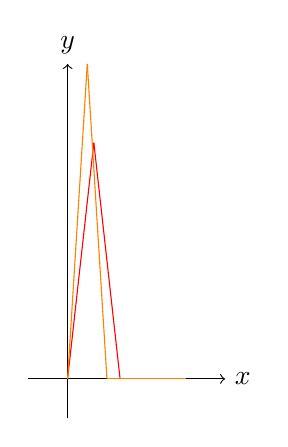
\begin{tikzpicture}
          \draw[->] (-0.5,0) -- (2,0) node[right] {$x$}; %
          \draw[->] (0,-0.5) -- (0,4) node[above] {$y$};%
          \draw [domain=0:1/3,red] plot (\x,3*3*\x);%
          \draw [domain=1/3:2/3,red] plot (\x,2*3-3*3*\x);%
          \draw [domain=2/3:1.5,red] plot (\x,0);%
 
          \draw [domain=0:1/4,orange] plot (\x,4*4*\x);%
          \draw [domain=1/4:2/4,orange] plot (\x,2*4-4*4*\x);%
          \draw [domain=2/4:1.5,orange] plot (\x,0);%
    \end{tikzpicture}
  \end{center}
\end{wrapfigure}

\begin{beispiele}
\item Sei $\MdQ\cap[0,1] = \{q_1, q_2, \ldots \}$, $f_n(x) = \begin{cases} 1, & x\in\{q_1,\ldots,q_n\} \\ 0, & x\in[0,1]\backslash\{q_1,\ldots,q_n\} \end{cases}$, $(n\in\MdN)$. $(f_n)$ konvergiert auf $[0,1]$ \emph{punktweise} gegen $f(x) = \begin{cases} 1, & x\in \MdQ \cap [0,1] \\ 0, & x \in [0,1]\backslash \MdQ \end{cases}$. Bekannt: $f \notin R[0,1]$. In 23.10 werden wir sehen: $f_n\in R[0,1] \ \forall n\in\MdN$.
\item Für $x\in[0,1]$, $n\in\MdN$, $n\ge 3$ sei $f_n$ wie in der Zeichnung:
$$f_n(x) = \begin{cases} n^2 x,& x\in[0,\frac{1}{n}] \\ 2n - n^2 x, & x\in(\frac{1}{n},\frac{2}{n}] \\ 0, & x \in (\frac{2}{n},1]\end{cases}$$
$f_n \in C[0,1] \folgt f_n \in R[0,1]$. zur Übung: $\int_0^1f_ndx = 1 \forall n\in\MdN$. $(f_n)$ konvergiert auf $[0,1]$ \emph{punktweise} gegen $f(x)= 0$. \\
Aber: $\lim_{n\to\infty}\int_0^1f_ndx = 1 \ne 0 = \int_0^1fdx = \int_0^1(\lim_{n\to\infty} f_n(x)) dx $
\end{beispiele}

\begin{satz}[Integrierbarkeit gleichmäßig konvergierender Funktionsfolgen]
$(f_n)$ sei eine Folge in $R[a,b]$ und $(f_n)$ konvergiert auf $[a,b]$ \emph{gleichmäßig} gegen $f:[a,b]\to\MdR$. Dann ist $f\in R[a,b]$ und 
$$\lim_{n\to\infty}\int_a^bf_n(x)dx  = \int_a^bfdx = \int_a^b(\lim_{n\to\infty} f_n)dx$$

$(f_n)$ sei eine Folge in $R[a,b]$ und $\sum_{n=1}^{\infty}f_n$ konvergiert auf $[a,b]$ \emph{gleichmäßig} gegen $f:[a,b]\to\MdR$. Dann ist $f\in R[a,b]$ und 
$$\sum_{n=1}^\infty \int_a^bf_n(x)dx = \int_a^b \sum_{n=1}^\infty f_n(x)dx $$
\end{satz}

\begin{beweis}
1. Zu $\ep=1 \ \exists m \in \MdN$: $f_m-1<f<f_m+1$ auf $[a,b]$. $f_n$ beschränkt auf $[a,b]$. \\
2. $A_n := \int_a^bf_ndx$ $(n\in\MdN)$. Sei $\ep>0$. $\exists n_0\in\MdN: f_n-\ep<f<f_n+\ep$ auf $[a,b] \ \forall n\ge n_0 \folgt$ für $n\ge n_0$ folgt (wie im Beweis von 23.2(1)): 
$$\underbrace{\uint_a^b(f_n-\ep)dx}_{=A_n-\ep(b-a)} \le \underbrace{\uint_a^bfdx}_{=: A} \le \underbrace{\oint_a^bfxds}_{=: B} \le \underbrace{\oint_a^b(f_n+\ep)dx}_{=A_n+\ep(b-a)}$$
$\folgt |A_n - A| \le \ep(b-a)$, $|A_n -B|\le \ep (b-a)$ \\ 
$\forall n\in n_0 \folgt A_n \to A, A_n \to B \ (n\to\infty) \folgt A = B $ \\ 
$\folgt f\in R[a,b]$ und $A_n \to \int_a^bfdx$
\end{beweis}

\begin{beispiel}
$$g(x) = \begin{cases} 0, & x=0 \\ 1, & x \in (0,1] \end{cases}$$
$g$ ist monoton $\folgt g \in R[0,1]$.
$$f(x) = \begin{cases} 1, & x=0 \\ 0, & x \in [0,1]\backslash\MdQ \\ \frac{1}{q}, & x = \frac{p}{q}, p,q \in \MdN \text{ teilerfremd} \end{cases}$$
Übungsblatt: $f\in R[0,1]$
$$(g\circ f)(x) = \begin{cases}1, &x\in Q\cap[0,1] \\ 0, & x \in [0,1]\backslash \MdQ \end{cases} \notin R[0,1]$$
\end{beispiel}

\begin{satz}[Integration von verketteten Funktionen]
Es sei $f\in R[a,b]$, $D := f([a,b])$ und $h: D \to R$ sei Lipschitzstetig auf $D$. Dann: $h\circ f \in R[a,b]$
\end{satz}

\begin{beweis}
$g:= h\circ f$. $\exists L>0$. $|h(t) - h(s)| \le L|t-s| \ \forall t,s \in D$. O.B.d.A: $L>0$. Sei $Z = \{x_0, \ldots, x_n\} \in \Z$, $m_j, M_j, I_j$ seien wie gehabt. $\tilde m_j := \inf g(I_j)$, $\tilde M_j := \sup g(I_j)$. Seien $x,y \in I_j$, etwa $f(x) \le f(y)$: $g(x) - g(y) \le |g(x) - g(<y|= |h(f(x)) - h(f(y))| \le L|f(x)-f(y)| = L(f(y)-f(x)) \le L(Mj-mj) =: c_j \folgt g(x) \le g(y) + c \ \forall x,y \in I_j \folgt \tilde M_j \le g(y)+c_j \ \forall y\in I_j \folgt \tilde M_j - c_j \le g(y) \ \forall y \in I_j \folgt \tilde M_j - c_j \le \tilde m_j \folgt \tilde M_j - \tilde m_j \le c_j = L(M_j - m_j) \folgt S_g(Z) - s_g(Z) = \sum_{j=1}^n(\tilde M_j - \tilde m_j)|I_j| \le L\sum_{j=1}^n(M_j - m_j)|I_j| = L(S_f(Z) - s_f(Z)) \ \forall z\in\Z \folgtnach{23.3} g\in R[a,b]$
\end{beweis}

\begin{satz}[Weitere Rechenregeln für Integrale]
Es seien $f,g \in R[a,b]$.
\begin{liste}
\item $|f| \in R[a,b]$ und $|\int_a^bfdx| \le \int_a^b|f|dx$ (\begriff{Dreiecksungleichung für Integrale})
\item $fg \in R[a,b]$
\item Ist $g(x) \ne 0 \ \forall x\in[a,b]$ und $\frac{1}{g}$ beschränkt auf $[a,b] \folgt \frac{1}{g} \in R[a,b]$
\end{liste}
\end{satz}

\begin{beweis}
\begin{liste}
\item $D:= f([a,b])$, $h(t) := |t| \ (t\in D)$. Dann: $|f|=h\circ f$. Für $t,s \in D$: $|h(t) - h(s)| = | |t| - |s| | \stackrel{\text{§1}}{\le} |t-s| \folgtnach{23.7} |f| \in R[a,b]$ \\
$ \pm f \le |f|$ auf $[a,b]$. 23.2 $\folgt \pm \int_a^bfdx \le \int_a^b|f|dx \folgt |\int_a^bfdx| \le \int_a^b|f|dx$
\item 1. $D:=f([a,b])$, $h(t) := t^2 \ (t\in D)$. Dann: $f^2 = h \circ f$.\\
$\exists \gamma >0: |f(x)|\le \gamma  \ \forall x\in[a,b] \folgt |t| < \gamma \ \forall t\in D$ Für $t, s \in D$: $|h(t)-h(s)| = |t^2 - s^2| = |t+s||t-s| \le (|t| + |s|)\cdot |t-s|\le 2\gamma |t-s| \folgtnach{23.7} f^2\in R[a,b]$\\
2. $f+g, f-g \in R[a,b] \folgt (f+g)^2,(f-g)^2 \in R[a,b] \folgt \frac{1}{4}\left( (f+g)^2 - (f-g)^2 \right) \in R[a,b] \folgt f\cdot g \in R[a,b]$
\item $D :=  g([a,b])$, $h(t) := \frac{1}{t}$ $(t\in D)$. Dann: $\frac{1}{g} = h \circ g$. \\
$\exists \gamma > 0: \frac{1}{|g(x)|} \le \gamma \ \forall x\in[a,b] \folgt \frac{1}{|t|} \le \gamma \ \forall t\in D$. Für $t,s \in D$: $|h(t) - h(s)| = |\frac{1}{t} - \frac{1}{s}| = \frac{|t-s|}{|t||s|}\le \gamma ^2 |t-s| \folgtnach{23.7} \frac{1}{g} \in R[a,b]$

\end{liste}
\end{beweis}

\begin{satz}[Aufteilung eines Integrals]
$f:[a,b] \to \MdR$ sei beschränkt und $c \in (a,b).$ Dann gilt:
$$f \in R[a,b] \equizu f \in R[a,c]\text{ und } f \in R[c,b].$$
In diesem Fall ist:
$$\intab{f} = \int_a^c{f\dx} + \int_c^b{f\dx}$$
\end{satz}

\def\hin{\item["`$\Rightarrow$"':]}
\def\zurueck{\item["`$\Leftarrow$"':]}

\begin{beweis}
\begin{description}
\hin Sei $\ep > 0.$ Aus 23.3 folgt: $\exists Z_1 \in \Z: S_f(Z_1) - s_f(Z_1) < \ep.$

$Z := Z_1 \cup \{c\} \in \Z.$ Sei $Z = \{x_0,\ldots,x_k,x_{k+1},\ldots,x_n\}$ mit $x_k = c.\ Z_0 := \{x_0,\ldots,x_k\}$ ist eine Zerlegung von $[a,c].\ M_j,\ m_j,\ I_j$ seien wie immer. Dann gilt:

$S_f(Z_0) - s_f(Z_0) = \sum_{j=1}^k{(M_j-m_j) |I_j|} \le \sum_{j=1}^n{(M_j-m_j) |I_j|} = S_f(Z)-s_f(Z) \le S_f(Z_1) - s_f(Z_1) < \ep \folgtnach{23.3} f \in R[a,c].$ Analog: $f \in R[c,b].$

\zurueck $S:=\int_a^c{f\dx} + \int_c^b{f\dx}.$ Sei $\ep > 0$ Dann gibt es Zerlegungen $Z_1$ von $[a,c]$ und $Z_2$ von $[c,b]: s_f(Z_1) = \uint_a^c{f\dx} - \ep = \int_a^c{f\dx},\ s_f(Z_2) > \int_b^c{f\dx} - \ep.$

$Z:=Z_1 \cup Z_2 \folgt Z \in \Z$ und $\uintab{f} \ge s_f(Z) = s_f(Z_1) + s_f(Z_2) > S-2 \ep.$

Also: $S-2\ep < \uintab{f}\ \forall \ep > 0 \folgtwegen{\ep \to 0+} S \le \uintab{f}.$

Analog: $\ointab{f} \le S \folgt f \in R[a,b],\ \intab{f} = S.$
\end{description}
\end{beweis}

\begin{satz}[Integral und Unstetigkeitsstellen]
$f,g: [a,b] \to \MdR$ seien Funktionen.
\begin{liste}
\item Ist $f$ beschränkt auf $[a,b]$ und $A:=\{x \in [a,b]: f$ ist in $x$ \emph{nicht} stetig$\}$ \emph{endlich}, dann gilt: $f \in R[a,b]$.
\item Ist $f \in R[a,b]$ und $A:=\{x \in [a,b]: f(x) \ne g(x)\}$ \emph{endlich}, dann gilt: $g \in R[a,b]$ und $\intab{g} = \intab{f}$.
\end{liste}
\end{satz}

\begin{beweise}
\item $\exists \gamma \ge 0: |f(x)| \le \gamma\ \forall x \in [a,b].$ Es genügt zu betrachten: $A:=\{t_0\}$ (wegen 23.9). O.B.d.A.: $t_0 = a$ oder $t_0 = b.$ Etwa: $t_0 = a$.

Sei $\ep > 0.$ Wähle $\alpha \in (a,b)$ mit $2\gamma(\alpha-a) < \ep/2.$

$f \in C[\alpha,b] \folgt f \in R[\alpha,b] \folgtnach{23.3}$ Es gibt eine Zerlegung $Z_1$ von $[\alpha,b]$ mit:\\ 
$S_f(Z_1) - s_f(Z_1) < \ep/2.\ Z:=Z_1 \cup \{a\} \folgt Z \in \Z$ und es gilt:\\
\begin{align*}
S_f(Z) - s_f(Z) &= \underbrace{\sup f([a,\alpha]) - \inf f([a,\alpha]))(\alpha-1)}_{\le 2 \gamma} + \underbrace{S_f(Z_1)-s_f(Z_1)}_{< \ep/2}\\
&< 2 \gamma(\alpha-a) + \ep/2 < \ep/2 + \ep/2 = \ep
\end{align*}

\item Klar: g ist beschränkt. $h := g-f.$ Dann: $h(x) = 0\ \forall x \in [a,b]\backslash A \folgt h \in C([a,b] \backslash A) \folgtnach{(1)} h \in R[a,b] \folgt g = h+f \in R[a,b].$

Noch zu zeigen: $\intab{h} = 0.\ \varphi := |h|.$ Aus 23.8 folgt: $\varphi \in R[a,b]$ und $|\intab{h}| \le \intab{\varphi}.$

Sei $Z := \{x_0,\ldots,x_n\} \in \Z,\ m_j := \inf \varphi(I_j),\ \varphi(x) = 0\ \forall x \in [a,b] \backslash A,\ \varphi(x) > 0\ \forall x \in A \folgt m_j = 0\ (j = 1,\ldots,n) \folgt s_f(Z) = 0 \folgt \uintab{\varphi} = \intab{\varphi} = 0 \folgt \intab{h} = 0.$
\end{beweise}

\begin{satz}[Mittelwertsatz der Integralrechnung]
Es seien $f,g \in R[a,b],\ g \ge 0$ (oder $g \le 0$) auf $[a,b],\ m:=\inf f([a,b]),\ M:=\sup f([a,b])$
\begin{liste}
\item $\exists \mu \in [m,M]: \intab{fg} = \mu \intab{g}$
\item Ist $f \in C[a,b] \folgt \exists \xi \in [a,b]: \intab{f} = f(\xi)(b-a)$
\end{liste}
\end{satz}

\begin{beweise}
\item $\alpha := \intab{g},\ \beta := \intab{fg}.\ m \le f \le M$ auf $[a,b] \folgt mg \le fg \le Mg$ auf $[a,b] \folgt m\alpha \le \beta \le M\alpha.$

Es ist $\alpha \ge 0.$ O.B.d.A.: $\alpha > 0.$ Dann gilt: $m \le \frac{\beta}{\alpha} \le M,\ \mu := \frac{\beta}{\alpha}.$

\item Setze in (1) $g \equiv 1 \folgt \intab{f} = \mu(b-a)\ (\mu \in [m,M]).$ Aus 18.1 folgt: $\exists \xi \in [a,b]: \mu = f(\xi).$
\end{beweise}

\paragraph{Der Riemannsche Zugang zum Integral}

\textit{Bemerkung: Wir haben bisher tatsächlich die \emph{Darbouxschen} Integrale betrachtet. Hier wird nun die ursprüngliche Definition von Riemann vorgestellt.}

$f:[a,b] \to \MdR$ sei beschränkt. Sei $Z:=\{x_0,\ldots,x_n\} \in \Z.\ m_j,M_j,I_j$ seien wie immer.

Wählt man in jedem $I_j$ einen Punkt $\xi_j$, so heißt $\xi := (\xi_1,\xi_2,\ldots,\xi_n)$ ein zu $Z$ passender \begriff{Zwischenvektor} und $\sigma_f(Z,\xi) := \sum_{j=1}^{n}{f(\xi_j) |I_j|}$ eine \begriff{Riemannsche Zwischensumme}.

$m_j \le f(\xi_j) \le M_j\ (j=1,\ldots,n) \folgt s_f(Z) \le \sigma_f(Z,\xi) \le S_f(Z)$

\begin{satz}[Äquivalenz der Riemannschen und Darbouxschen Integrale]
$f: [a,b] \to \MdR$ sei beschränkt. Dann gilt: $f \in R[a,b]$ genau dann, wenn es ein $S \in \MdR$ gibt mit:
$$\forall \ep > 0\ \exists Z \in \Z: |\sigma_f(Z,\xi)-S| < \ep\text{ für jedes zu Z passende } \xi.\ (*)$$
In diesem Fall gilt:
$$S = \intab{f}.$$
\end{satz}

\begin{beweis}
\begin{description}
\hin $S := \intab{f}.$ Sei $\ep > 0.$ Wie im Beweis von 23.3: $\exists Z \in \Z: s_f(Z) > S-\ep,\ S_f(Z) < S+\ep.$

Sei $\xi$ passend zu $Z \folgt S-\ep < s_f(Z) \le \sigma_f(Z,\xi) \le S_f(Z) < S+\ep \folgt |\sigma_f(Z,\xi)-S| < \ep.$

\zurueck Sei $\ep > 0.$ Nach Voraussetzung gibt es ein $Z \in \Z$ so, dass ($*$) gilt. Sei $Z := \{x_0,\ldots,x_n\},\ m_j,\ M_j,\ I_j$ wie immer. Sei $j \in \{1,\ldots,n\}: \exists \xi_j,\eta_j \in I_j: f(\xi_j) > M_j - \ep,\ f(\eta_j) < m_j + \ep,\ \xi := (\xi_1,\ldots,\xi_n),\ \eta = (\eta_1,\ldots,\eta_n)$ sind passend zu $Z$.

$A := \sigma_f(Z,\xi),\ B := \sigma_f(Z,\eta).\ A = \sum_{j=1}^n{f(\xi_j) |I_j|} > \sum_{j=1}^n{(M_j-\ep) |I_j|} = S_f(Z) - \ep(b-a) \folgt S_f(Z) < A + \ep(b-a).\quad$(i)

Analog: $-s_f(Z) < \ep(b-a) - B.\quad$(ii)

Dann gilt: $S_f(Z) - s_f(Z) < A-B+2\ep(b-a) = A-S+S-B+2\ep(b-a) \le |A-S|+|B-S|+2\ep(b-a) \overset{\text{($*$)}}{<} 2\ep+2\ep(b-a) = \ep(2 + 2(b-a)) \folgtnach{23.3} f \in R[a,b].$

$\intab{f} = \ointab{f} \le S_f(Z) \overset{\text{(i)}}{<} A + \ep(b-a) = A - S + S + \ep(b-a) \le |A-S| + S + \ep(b-a) \overset{\text{($*$)}}{<} \ep + S + \ep(b-a).$

Also: $\intab{f} < S + \ep(1 + (b-a))\ \forall \ep > 0 \folgtwegen{\ep \to 0+} \intab{f} \le S.$ Analog folgt mit (ii): $S \le \intab{f}.$
\end{description}
\end{beweis}

\begin{definition}
Sei $f \in R[a,b].\ \int_c^cf(x)\dx:=0$ und $\int_b^af(x)\dx=:-\int_a^bf(x)\dx$
\end{definition}
\begin{bemerkung}
$\int_a^bf(x)\dx=\int_a^bf(t)\dt$.
\end{bemerkung}

\begin{satz}[2. Hauptsatz der Differential- und Integralrechnung]
Sei $f \in R[a,b]$ und $F:[a,b]\to\MdR$ sei definiert durch $F(x):=\int_a^xf(t)\dt$.
\begin{liste}
\item $F$ ist auf $[a,b]$ Lipschitzstetig, insbesondere $F \in C[a,b]$
\item Ist $f$ in $x_0 \in [a,b]$ stetig $\folgt F$ ist in $x_0$ differenzierbar und $F'(x_0)=f(x_0)$
\item Ist $f \in C[a,b] \folgt F \in C^1[a,b]$ und $F'=f$ auf $[a,b]$
\end{liste}
\end{satz}

\begin{beweise}
\item $L:=\sup\{|f(x)| : x \in [a,b]\}$. Sei $x,y \in [a,b]$, etwa $x\le y$. $F(y)=\int_a^yf(t)\dt\gleichnach{23.9}\int_a^xf(t)\dt + \int_x^yf(t)\dt=F(x)+\int_x^yf(t)\dt\folgt F(y)-F(x)=\int_x^yf(t)\dt\folgt |F(y)-F(x)|=|\int_x^yf(t)\dt|\overset{23.8}{\le}\int_x^y\underbrace{|f(t)|}_{\le L}\dt\le\int_x^yL\dt=L(y-x)=L|y-x|$
\item Sei $x_0 \in [a,b)$. Wir zeigen: $(*) \displaystyle\lim_{h\to 0+}\frac{F(x_0+h)-F(x_0)}{h}=f(x_0)$ (analog zeigt man f"ur $x_0 \in (a,b]\ :\ \displaystyle\lim_{h\to0-}\frac{F(x_0+h)-F(x_0)}{h}=f(x_0)$) Sei also $x_0 \in [a,b)$, $h>0$ und $x_0+h<b$. $g(h):=|\frac{F(x_0+h)-F(x_0)}{h}-f(x_0)|$. Zu zeigen: $g(h)\to 0\ (h\to0+)$. Es ist $\frac{F(x_0+h)-F(x_0)}{h}\gleichnach{s.o.}\frac{1}{h}\int_{x_0}^{x_0+h}f(t)\dt$, $\ \frac{1}{h}\int_{x_0}^{x_0+h}f(x_0)\dt=\frac{1}{h}f(x_0)h=f(x_0)\folgt g(h)=\frac{1}{h}|\int_{x_0}^{x_0+h}(f(t)-f(x_0))\dt|\overset{23.8}{\le}\frac{1}{h}\int_{x_0}^{x_0+h}|f(t)-f(x_0)|\dt;\ s(h):=\sup\{|f(t)-f(x_0)|\ :\ t \in [x_0,x_0+h]\}\folgt g(h)\le\frac{1}{h}\int_{x_0}^{x_0+h}s(h)\dt=\frac{1}{h}s(h)h=s(h)$. Also: $0\le g(h)\le s(h)$. $f$ stetig in $x_0 \folgt f(t)\to f(x_0)\ (t \to x_0) \folgt s(h)\to 0\ (h\to 0+) \folgt g(h)\to 0\ (h\to 0+)\folgt (*)$
\item folgt aus (2)
\end{beweise}

\begin{satz}[Anwendung des 2. Hauptsatzes auf stetige Funktionen]
Sei $J \subseteq \MdR$ ein beliebiges Intervall, $f \in C(J)$ und $\xi \in J$ (fest). $F:J\to\MdR$ sei definiert durch $F(x):=\int_{\xi}^xf(t)\dt$. Dann ist $F\in C^1(J)$ und $F'=f$ auf $J$. 
\end{satz}


\begin{beweis}
Seien $a,b \in J$, $a<b$ und $I:=[a,b]$. Es gen"ugt zu zeigen: $F$ ist differenzierbar auf $I$ und $F'=f$ auf $I$. $G(x):=\int_a^xf(t)dt\ (x\in I)$. Sei $\xi\le a$ (analoger Beweis f"ur $\xi\ge b$ und $\xi \in (a,b)$. F"ur $x \in [a,b]:\ F(x)=\int_{\xi}^x\cdots = \int_{\xi}^a\cdots + \int_a^x\cdots=F(a)+G(x)\folgtnach{23.13} F$ ist differenzierbar auf $I$ und $F'=G'=f$ auf $I$.
\end{beweis}

\begin{definition}
Im folgenden seien $I,J\subseteq\MdR$ beliebige Intervalle.
\begin{liste}
\item Sei $g:I\to\MdR$ und $x_0\in I$. $g(x)|_{x=x_0}:=g(x_0).$
\item Ist $f \in R[a,b]$, so hei"st $\int_a^bf(x)\dx$ auch ein \begriff{bestimmtes Integral}.
\item Besitzt $G:I\to\MdR$ auf $I$ eine Stammfunktion, so schreibt man f"ur eine solche auch $\int g(x)\dx$ (\begriff{unbestimmtes Integral}). "Gleichungen" der Form $\int g(x)\dx=h(x)$ gelten bis auf additive Konstanten! \textbf{Beispiel}: $\int e^x\dx=e^x, \int e^x\dx=e^x + 7$. $\int g(x)\dx=h(x)$ auf $I$ bedeutet: h ist eine Stammfunktion von $g$ auf $I$.
\end{liste}
\end{definition}

\begin{satz}[Partielle Integration]
\begin{liste}
\item Es seien $f,g \in R[a,b]$ und $F,G$ seien Stammfunktionen von $f$ bzw. $g$ auf $[a,b]$. Dann: $$\int_a^bFg\dx=F(x)G(x)|_a^b-\int_a^bfG\dx$$
\item Sind $f,g \in C^1[a,b] \folgt$ $$\int_a^b f'g\dx=f(x)g(x)|_a^b-\int_a^bfg'\dx$$
\item Sind $f,g \in C^1(I) \folgt$ auf $I$ gilt: $$\int f'g\dx=f(x)g(x)-\int fg'\dx$$
\end{liste}
\end{satz}

\begin{beweise}
\item $(FG)'=F'G+FG'=fG+Fg\folgt \int_a^bFg\dx+\int_a^bfG\dx=\int_a^b(FG)'\dx\gleichnach{23.5}F(x)G(x)|_a^b$
\item folgt aus (1)
\item $(fg)'=f'g+fg'\folgt fg=\int(f'g+fg')\dx$
\end{beweise}

\begin{beispiele}
\item $\int \log x\dx=\int\underbrace{1}_{f'}\underbrace{\log x}_{g}\dx=x\log x-\int x\frac{1}{x}dx=x\log x - x$ auf $(0, \infty)$.
\item $\int \sin^2 x\dx = \int\underbrace{\sin x}_{f'}\underbrace{\sin x}_{g}\dx = -\cos x\sin x - \int{-\cos^2 x\dx}=-\cos x\sin x + \int(1-\sin^2 x)\dx=-\cos x\sin x + x-\int\sin^2 x\dx$

$\folgt \int\sin^2\dx =\frac{1}{2}(x-\cos x \sin x)$ auf $\MdR$.
\item $\int \underbrace{x}_{f'}\underbrace{e^x}_{g}\dx=\frac{1}{2}x^2e^x-\int\frac{1}{2}x^2e^x\dx$ \emph{komplizierter!}\\
$\int\underbrace{x}_{f}\underbrace{e^x}_{g'}=xe^x-\int{e^x\dx}=xe^x-e^x$
\end{beispiele}

\begin{satz}[Substitutionsregeln]
Sei $f\in C(I)$ und $g \in C^1(J)$ und $g(J)\subseteq I$.
\begin{liste}
\item Ist $J=[\alpha, \beta]\folgt$ $$\int_{\alpha}^{\beta}f(g(t))g'(t)\dt=\int_{g(\alpha)}^{g(\beta)}f(t)\dt$$
\item Auf $J$ gilt: $$\int f(g(t))g'(t)\dt=\int f(x)\dx|_{x=g(t)}$$
\item $g$ sei auf $J$ streng monoton $\folgt$ auf $I$ gilt: $$\int f(x)\dx=\int f(g(t))g'(t)\dt|_{t=g^{-1}(x)}$$.
\end{liste}
\end{satz}

\begin{merkregel}
Ist $y=y(x)$ differenzierbar, so schreibt man f"ur $y'$ auch $\frac{dy}{dx}$. In 23.16 substituiere $x=g(t)$ (fasse also $x$ als Funktion von $t$ auf) $\folgt g'(t)=\frac{dx}{dt}$ \glqq$\folgt dx=g'(t)dt$\grqq.
\end{merkregel}

\begin{beweise}
\item[(2)]
Sei $F$ eine Stammfunktion von $f$ auf $I$. $G(t):=F(g(t))\ (t\in J)$. $G'(t)=F'(g(t))g'(t)=f(g(t))g'(t)\ (t\in J)\folgt G$ ist eine Stammfunktion von $(f\circ g)g'$ auf $J \folgt$ (2)
\item[(1)]$\int_{\alpha}^{\beta}f(g(t))g'(t)\dt\overset{23.5}{=}G(\beta)-G(\alpha)=F(g(\beta))-F(g(\alpha))\overset{23.5}{=}\int_{g(\alpha)}^{g(\beta)}f(x)\dx$.
\item[(3)]$\int f(g(t))g'(t)\dt|_{t=g^{-1}(x)}=G(g^{-1}(x))=F(g(g^{-1}(x)))=F(x)$
\end{beweise}

\begin{beispiele}
\item $\int_0^1\sqrt{1-x^2}\dx$ (Substitution $x=\sin t,\ t=0\folgt x=0,\ t=\frac{\pi}{2}\folgt x=1,\dx=\cos t\dt$). $\int_0^1\sqrt{1-x^2}\dx=\int_0^{\frac{\pi}{2}}\sqrt{1-\sin^2 t}\cos t\dt=\int_0^\frac{\pi}{2}|\cos t|\cos t\dt=\int_0^{\frac{\pi}{2}}\cos^2t\dt=\int_0^{\frac{\pi}{2}}(1-\sin^2t)\dt=t-\frac{1}{2}(t-\cos t\sin t)|_0^{\frac{\pi}{2}}=\frac{\pi}{4}$.
\item $\int\frac{1}{x\log x}\dx$ (Substitution $x=e^t,\ t=\log x,\dt=\frac{1}{x}\dx$). $\int\frac{1}{x\log x}=\int\frac{1}{t}\dt=\log t=\log(\log(x))$ auf $(1,\infty)$.
\end{beispiele}

\begin{definition}
\begin{liste}
\item Seien $p$ und $q$ Polynome und $q \neq 0.$ Dann heißt $\frac{p}{q}$ eine \begriff{rationale Funktion}.

$\frac{p}{q}$ hat eine Darstellung der Form $\frac{p}{q} = p_1 + \frac{p_2}{q}$, wobei $p_1,p_2$ Polynome und $\frac{p_2}{q}$ \begriff{echt gebrochen rational}, d.h.: $\text{Grad } p_2 < \text{Grad } q$.

\item Seien $b,c \in \MdR$. Dann heißt das Polynom $x^2+bx+c$ \begriff{unzerlegbar} über $\MdR :\equizu 4c-b^2 > 0\quad(\equizu x^2+bx+c \ne 0\ \forall x \in \MdR)$

\item Ein \begriff{Partialbruch} ist eine rationale Funktion der Form $$\frac{A}{(x-x_0)^k}$$wobei $A,x_0 \in \MdR,\ k \in \MdN$, oder $$\frac{Ax+B}{(x^2+bx+c)^k}$$wobei $A,B,b,c \in \MdR,\ k \in \MdN$ und $x^2+bx+c$ unzerlegbar über \MdR.
\end{liste}
\end{definition}

\newcommand{\fint}[2]{\int{\frac{#1}{#2}\dx}}

\begin{satz}[Integration von rationalen Funktionen]
Es seien $b,c,x_0 \in \MdR,\ m \in \MdN,\ m > 1,\ p(x) := x^2+bx+c$ und $D := 4c-b^2 > 0$
\begin{liste}
\item $\displaystyle{\fint{1}{x-x_0} = \log{|x-x_0|}}$
\item $\displaystyle{\fint{1}{(x-x_0)^m} = \frac{-1}{m-1} \cdot \frac{1}{(x-x_0)^{m-1}}}$
\item $\displaystyle{\fint{1}{p(x)} = \frac{2}{\sqrt{D}} \arctan{\left( \frac{2x+b}{\sqrt{D}} \right)}}$
\item $\displaystyle{\fint{1}{p(x)^m} = \frac{1}{(m-1)D} \cdot \frac{2x+b}{p(x)^{m-1}} + \frac{4m-6}{(m-1)D} \fint{1}{p(x)^{m-1}}}$
\item $\displaystyle{\fint{x}{p(x)} = \frac{1}{2} \log{(p(x))} - \frac{b}{2} \fint{1}{p(x)}}$
\item $\displaystyle{\fint{x}{p(x)^m} = \frac{-1}{2(m-1)} \cdot \frac{1}{p(x)^{m-1}} - \frac{b}{2} \fint{1}{p(x)^m}}$
\end{liste}
\end{satz}

\begin{beweise}
\item klar
\item klar
\item  $p(x) = x^2+bx+c = x^2+bx+\frac{b^2}{4} + c - \frac{b^2}{4} = (x+\frac{b}{2})^2 + \frac{D}{4} = \frac{D}{4}(\frac{4}{D}(x+\frac{b}{2})^2 + 1) = \frac{D}{4}((\frac{2x+b}{\sqrt{D}})^2 + 1)= \frac{D}{4}(t^2+1),$ wobei $t = \frac{2x+b}{\sqrt{D}},$ also $x = \frac{\sqrt{D}t - b}{2}$

$\folgt \int\frac{1}{p(x)}\dx =$ (Substitution $t=\frac{2x+b}{\sqrt{D}},\  dx=\frac{\sqrt{D}}{2}\dt$) $\frac{4}{D} \int\frac{1}{t^2+1} \cdot \frac{\sqrt{D}}{2}\dt = \frac{2}{\sqrt{D}} \int\frac{1}{1+t^2}\dt = \frac{2}{\sqrt{D}} \arctan t = \frac{2}{\sqrt{D}} \arctan(\frac{2x+b}{\sqrt{D}})$

\item Übung, partielle Integration
\item $\int\frac{x}{p(x)}\dx = \frac{1}{2} \int\frac{2x+b-b}{p(x)}\dx = \frac{1}{2}\int \underbrace{\frac{p'(x)}{p(x)}}_{\log(p(x))}\dx - \frac{b}{2} \int\frac{1}{p(x)}\dx$

\item Übung, partielle Integration
\end{beweise}

\begin{definition}
\begin{liste}
\item Sei $Z = \{x_0,\ldots,x_n\} \in \Z,\ I_j = [x_{j-1},x_j]\ (j=1,\ldots,n)$

$|Z| := \max \{|I_j| : j=1,\ldots,n\}$ heißt das \begriff{Feinheitsmaß} von $Z$.

\item $\Z^* := \{(Z,\xi) : Z \in \Z,\ \xi$ ist passend zu $Z \}$. Eine Folge $((Z_n,\xi^{(n)}))$ in $\Z^*$ heißt eine \begriff{Nullfolge} $:\equizu |Z_n| \to 0\ (n \to \infty)$
\end{liste}
\end{definition}

\begin{satz}[Folgen von Zerlegungen mit $|Z_n| \to 0$]
$f: [a,b] \to \MdR$ sei beschränkt; sei $\gamma \ge 0$ mit: $|f(x)| \le \gamma\ \forall x \in [a,b].$
\begin{liste}
\item Sind $Z_1,Z_2 \in \Z$ und $Z_1 \subseteq Z_2$ und enthält $Z_2$ genau $p$ Teilpunkte mehr als $Z_1$, dann gilt: $$s_f(Z_2) \le s_f(Z_1) + 2p\gamma|Z_1|\text{ und}$$
$$S_f(Z_2) \ge S_f(Z_1) - 2p\gamma|Z_1|.$$

\item $\forall \ep > 0\ \exists \delta > 0\ \forall Z \in \Z$ mit $|Z| < \delta$: $$s_f(Z) > \uintab{f} - \ep,\ S_f(Z) < \ointab{f} + \ep.$$

\item Ist $(Z_n)$ eine Folge in $\Z$ mit $|Z_n| \to 0$, dann gilt: $$s_f(Z_n) \to \uintab{f},\ S_f(Z_n) \to \ointab{f}.$$
\end{liste}
\end{satz}

\begin{beweise}
\item Übung, es genügt den Fall $p=1$ zu betrachten.
\item Beweis nur für Untersummen. Sei $\ep > 0.\ \exists Z_1 \in \Z: s_f(Z_1) > \uintab{f} - \frac{\ep}{2};\ Z_1$ habe $p$ Teilpunkte. $\delta := \frac{\ep}{4\gamma p}.$

Sei $Z \in \Z$ und $|Z| < \delta.\ Z_2 := Z \cup Z_1 \in \Z;\ Z_2$ hat höchstens $p$ Teilpunkte mehr als $Z \folgt s_f(Z) = \underbrace{s_f(Z) - s_f(Z_2)}_{\underset{\text{(1)}}{>} -2p\gamma|Z|} + \underbrace{s_f(Z_2)}_{\ge s_f(Z_1)} > -2p\gamma|Z| + s_f(Z_1) > -\underbrace{2\gamma p \delta}_{=\frac{\ep}{2}} + \uintab{f} - \frac{\ep}{2} = \uintab{f} - \ep.$

\item Nur für Untersummen. $A := \uintab{f},\ s_n := s_f(Z_n).$ Sei $\ep > 0.$ Aus (2) folgt dann: $\exists \delta > 0: s_f(Z) > A-\ep\ \forall Z \in \Z$ mit $|Z| < \delta.\ \exists n_0 \in \MdN: |Z_n| < \delta\ \forall n \ge n_0.$ Also: $s_n \to A\quad(n \to \infty).$

\end{beweise}

\begin{beispiel}
$$a_n := \sum_{j=1}^n{\frac{\sqrt{j}}{n^{3/2}}}.\text{ Behauptung}: a_n \to \frac{2}{3}$$
\begin{beweis}
$$a_n = \sum_{j=1}^n{\underbrace{\sqrt{\frac{j}{n}}}_{= f(\frac{j}{n})} \frac{1}{n}},\ f(x) = \sqrt{x},\ x \in [0,1].$$

$Z_n = \{0,\frac{1}{n},\ldots,\frac{n}{n}\} \folgt a_n = S_f(Z_n) \underset{\text{23.18(3)}}{\overset{n \to \infty}{\to}} \uint_0^1\sqrt{x}\dx = \int_0^1 \sqrt{x}\dx = \frac{2}{3}$
\end{beweis}
\end{beispiel}

\begin{satz}[Riemannsche Definition des Integrals mit Nullfolgen]
$f: [a,b] \to \MdR$ sei beschränkt. $f \in R[a,b] \equizu \exists S \in \MdR: \sigma_f(Z_n,\xi^{(n)}) \to S\ (n \to \infty)$ für jede Nullfolge $((Z_n,\xi^{(n)})) in \Z^*.$ In diesem Fall gilt: $S = \intab{f}$.
\end{satz}

\begin{beweis}
\begin{description}
\hin $S := \intab{f}$. Sei $((Z_n,\xi^{(n)})) \in \Z^*$ eine Nullfolge. Dann: $$\underbrace{s_f(Z_n)}_{\overset{\text{23.18}}{\to}S}  \le \sigma_f(Z_n,\xi^{(n)}) \le \underbrace{S_f(Z_n)}_{\overset{\text{23.18}}{\to}S}\ \forall n \in \MdN.$$

$\folgt \sigma_f(Z_n,\xi^{(n)}) \to S\ (n \to \infty)$.

\zurueck Sei $\ep > 0$ und $(Z_n)$ eine Folge in $\Z$ mit $|Z_n| \to 0.$ Wie im Beweis von 23.12: $\forall n \in \MdN\ \exists \xi^{(n)},\eta^{(n)}$ passend zu $Z_n$ mit: $$S_f(Z_n) - \ep < \sigma_f(Z_n,\xi^{(n)});\ \sigma(Z_n,\eta^{(n)}) < s_f(Z_n) + \ep$$

Aus 23.18(3) folgt für $n \to \infty:\ \ointab{f} - \ep \le S \le \uintab{f} + \ep\ \forall \ep > 0 \folgtwegen{\ep \to 0+} \ointab{f} \le S \le \uintab{f} \folgt f \in R[a,b]$ und $\intab{f} = S$.
\end{description}
\end{beweis}

\begin{beispiel}
\textit{Bemerkung: Dies ist ein Beispiel zum nächsten Satz, nicht zum vorherigen.}

$f_n(x) = \frac{1}{n} \sin (nx)\ (n \in \MdN,\ x \in [0,\pi]);\ |f_n(x)| = \frac{1}{n} |\sin(nx)| \le \frac{1}{n}\ \forall x \in [0,\pi].$

$\folgt (f_n)$ konvergiert gleichmäßig auf $[0,\pi]$ gegen $f \equiv 0$.

$f_n'(x) = \cos(nx),\ f_n'(\pi) = \cos(n\pi) = (-1)^n.$ Das heißt: $(f_n')$ konvergiert auf $[0,\pi]$ \emph{nicht} punktweise.
\end{beispiel}

\begin{satz}[Gleichmäßige Konvergenz der Stammfunktion]
$(f_n)$ sei eine Folge in $C^1[a,b],\ x_0 \in [a,b]$ und es gelte:
\begin{itemize}
\item[(i)] $(f_n(x_0))$ konvergiert
\item[(ii)] $(f_n')$ konvergiert gleichmäßig auf $[a,b]$ gegen $g:[a,b] \to \MdR.$
\end{itemize}

Dann konvergiert $(f_n)$ gleichmäßig auf $[a,b]$ und für $f(x) := \lim_{n\to\infty} f_n(x)\ (x \in [a,b])$ gilt: $f \in C^1[a,b]$ und $f'=g$ auf $[a,b].$

Also: $(\lim_{n\to\infty} f_n(x))' = f'(x) = g(x) = \lim_{n\to\infty} f_n'(x)\ \forall x \in [a,b].$
\end{satz}

\newcommand{\gehtwegen}[1]{\overset{#1}{\to}}
\newcommand{\gehtnach}[1]{\overset{\text{#1}}{\to}}

\begin{beweis}
O.B.d.A.: $x_0=a$ und $f_n(a) \to 0\ (n \to \infty).\ f(x):=\int_a^x g(t)\dt\ (x \in [a,b]).$ Aus 19.2 folgt: $g \in C[a,b].$

Damit wegen 23.13: $f \in C^1[a,b]$ und $f'=g$ auf $[a,b].$

Sei $x \in [a,b]: f_n(x) - \underbrace{f_n(a)}_{\to 0} \gleichnach{23.5} \int_a^x f_n'(t)\dt \gehtnach{23.6} \int_a^x g(t)\dt = f(x).$

$\folgt (f_n)$ konvergiert punktweise gegen $f$.

Für $x \in [a,b]: |f_n(x)-f(x)| = |f_n(x)-f_n(a)-f(x)+f_n(a)| = |\int_a^x (f_n'(t)-g(t))\dt + f_n(a)| \le \int_a^x |f_n'-g|\dt + |f_n(a)| \le \int_a^b |f_n'-g|\dt + |f_n(a)| =: c_n$

Wegen Voraussetzung (ii) konvergiert $(|f_n'-g|)$ auf $[a,b]$ gleichmäßig gegen $0$. Wegen 23.6 folgt damit: $\int_a^b |f_n'-g| \dt \to 0\ (n \to \infty) \folgt c_n \to 0\ (n \to \infty) \folgt (f_n)$ konvergiert gleichmäßig auf $[a,b]$ gegen $f$.
\end{beweis}

Wir können nun den Satz 21.9 beweisen.

\begin{beweis}
Sei $a<b$ und $[a,b] \subseteq I.\ f_n(x) := \sum_{k=0}^n a_k x^k,\ f_n'(x) = \sum_{k=1}^n ka_kx^{k-1},\ g(x) := \sum_{k=1}^\infty ka_kx^{k-1}$

Aus 19.1 folgt: $(f_n)$ und $(f_n')$ konvergieren auf $[a,b]$ gleichmäßig gegen $f$ bzw. $g$. Wegen unserem neuen Satz 23.20 nun ist $f$ auf $[a,b]$ differenzierbar und $f'=g$ auf $[a,b]$. $[a,b] \subseteq I$ beliebig $\folgt$ Beh.
\end{beweis}

\chapter{Uneigentliche Integrale}

In diesem Paragraphen gelte stets: Ist $I \subseteq \MdR$ ein Intervall und $\varphi: I \to \MdR$ eine Funktion, so gelte $\varphi \in R[a,b]$ für jedes Intervall $[a,b] \subseteq I$.

\paragraph{(I) 1. Typ uneigentlicher Integrale}
Sei $a \in \MdR,\ \beta \in \MdR \cup \{\infty\},\ a<\beta$ und $f:[a,\beta) \to \MdR.$ Existiert der Grenzwert $\lim_{t\to\beta} \int_a^t f(x)\dx$ und ist dieser Grenzwert reell, so heißt das \begriff{uneigentliche Integral} $\int_a^\beta f(x)\dx$ \begriff{konvergent} und $\int_a^\beta f(x)\dx := \lim_{t\to\beta} \int_a^t f(x)\dx.$ Ist das Integral $\int_a^\beta f\dx$ nicht konvergent, so heißt es \begriff{divergent}.

\begin{beispiele}
\item $$\int_0^1 \frac{1}{\sqrt{1-x^2}}\dx\quad(a=0,\beta=1)$$

Für $t \in (0,1): \int_0^t \frac{1}{\sqrt{1-x^2}}\dx = \arcsin|_0^t = \arcsin t \to \frac{\pi}{2}\ (t \to 1).$ Das heißt: $\int_0^1 \frac{1}{\sqrt{1-x^2}}\dx$ konvergiert und hat den Wert $\frac{\pi}{2}$.

\item $$\int_0^\infty \frac{1}{1+x^2}\dx\quad(a=0,\beta=\infty)$$

Für $t>0: \int_0^t \frac{1}{1+x^2}\dx = \arctan x|_0^t = \arctan t \to \frac{\pi}{2}\ (t \to \infty)$. Also: $\int_0^\infty \frac{1}{1+x^2}\dx$ konvergiert und hat den Wert $\frac{\pi}{2}$.

\item \textit{(wichtig)} Sei $\alpha > 0$. Übung: $$\int_1^\infty \frac{1}{x^\alpha}\dx\text{ konvergiert} \equizu \alpha > 1$$
\end{beispiele}

\paragraph{(II) 2. Typ uneigentlicher Integrale}
Sei $\alpha \in \MdR \cup \{-\infty\},\ a \in \MdR,\ \alpha < a$ und $f:(\alpha,a] \to \MdR$ eine Funktion. Entsprechend zum 1. Typ definiert man die Konvergenz bzw. Divergenz des uneigentlichen Integrals $\int_\alpha^a f(x) \dx$ (nämlich $\lim_{t\to\alpha} \int_t^a f(x)\dx).$

\begin{beispiele}
\item $$\int_{-\infty}^0 \frac{1}{1+x^2}\dx$$

Für $t<0: \int_t^0 \frac{1}{1+x^2}\dx = \arctan x|_t^0 = -\arctan t = \arctan (-t) \to \frac{\pi}{2}\ (t \to -\infty)$

\item \textit{(wichtig)} Sei $\alpha > 0.$ Übung: $$\int_0^1 \frac{1}{x^\alpha}\dx\text{ konvergiert} \equizu \alpha < 1$$
\end{beispiele}

\paragraph{(III) 3. Typ uneigentlicher Integrale}
Sei $\alpha \in \MdR \cup \{-\infty\},\ \beta \in \MdR \cup \{-\infty\},\ \alpha < \beta$ und $f:(\alpha,\beta) \to \MdR$ eine Funktion. Das uneigentliche Integral $\int_\alpha^\beta f(x)\dx$ ist \begriff{konvergent}, genau dann wenn es ein $c \in (\alpha,\beta)$ gibt mit: $\int_\alpha^c f(x)\dx$ konvergiert \emph{und} $\int_c^\beta f(x)\dx$ konvergiert. In diesem Fall gilt: $\int_\alpha^\beta f\dx := \int_\alpha^c f\dx + \int_c^\beta f\dx$ (Übung: diese Definition ist unabhängig von $c$)

\begin{beispiele}
% Fehlt hier was?
\item $\int_{-\infty}^\infty\frac{1}{1+x^2}\dx$ konvergiert und hat den Wert $\pi$.

\item $\int_0^\infty \frac{1}{x^2}\dx$ divergiert, denn $\int_0^1 \frac{1}{x^2}\dx$ divergiert.
\end{beispiele}

Das Folgende formulieren wir nur für den Typ (I) (sinngemäß gilt alles auch für Typ (II), (III)):

\begin{definition}
$\int_a^\beta f\dx$ heißt \begriff{absolut konvergent} $:\equizu \int_a^\beta |f|\dx$ ist konvergent.
\end{definition}

\begin{satz*}
Sei $g:[a,\beta) \to \MdR$ eine weitere Funktion.
\begin{liste}
\item $\int_a^\beta f\dx$ konvergiert $\equizu \exists c \in (a,\beta): \int_c^\beta f\dx$ konvergiert.

In diesem Fall gilt: $\int_a^\beta f\dx = \int_a^c f\dx + \int_c^\beta f\dx.$

\item \begriff{Cauchykriterium}: $\int_a^\beta f\dx$ konvergiert $\equizu \forall \ep>0\ \exists c=c(\ep) \in (a,\beta): |\int_u^v f\dx| < \ep\ \forall u,v \in (c,\beta)$

\item Ist $\int_a^\beta f\dx$ absolut konvergent, dann gilt: $\int_a^\beta f\dx < \int_a^\beta |f|\dx$ und $|\int_a^\beta f\dx| < \int_a^\beta |f|\dx$.

\item \begriff{Majorantenkriterium}: Ist $|f| \le g$ auf $[a,\beta)$ und $\int_a^\beta g\dx$ konvergent, dann konvergiert $\int_a^\beta f\dx$ absolut.

\item \begriff{Minorantenkriterium}: Ist $f \ge g \ge 0$ auf $[a,\beta)$ und $\int_a^\beta g\dx$ divergent, dann divergiert $\int_a^\beta f\dx$.
\end{liste}
\end{satz*}

\begin{beispiele}
\item $\int_1^\infty \underbrace{\frac{x}{1+x^2}}_{=:f(x)}\dx,\ g(x) := \frac{1}{x}.\ \frac{f(x)}{g(x)} = \frac{x^2}{1+x^2} \to 1\ (x\to\infty).$

$\folgt \exists c \in (1,\infty): \frac{f(x)}{g(x)} \ge \frac{1}{2}\ \forall x \ge c \folgt f(x) \ge \frac{1}{2x}\ \forall x \ge c.\ \int_c^\infty \frac{1}{2x}\dx$ divergiert $\folgt \int_c^\infty f(x)\dx$ divergiert $\folgt \int_1^\infty f(x)\dx$ divergiert.

\item $f(x) = \frac{1}{\sqrt{x}}.\ \int_0^1 f(x)\dx$ konvergiert, $\int_0^1 f^2(x)\dx$ divergiert.
\end{beispiele}

\def\Z{\ensuremath{\mathfrak{Z}}}
\def\hin{\item["`$\Rightarrow$"':]}
\def\zurueck{\item["`$\Leftarrow$"':]}
\def\BV{\text{BV}}
\def\dx{\text{d}x}

\chapter{Funktionen von beschränkter Variation}

\begin{definition}
Sei $f:[a,b]\to\MdR$ und $Z=\{x_0,\ldots,x_n\} \in\Z$. $V_f(Z):=\sum_{j=1}^n|f(x_j)-f(x_{j-1})|$ ist die \begriff{Variation} von $f$ bez"uglich Z.\\
\textbf{Beachte}: Sind $Z_1,Z_2 \in \Z$ und $Z_1 \subseteq Z_2\folgt V_f(Z_1) \le V_f(Z_2)$. $M_f=\{V_f(Z):Z \in \Z\}.\ f$ hei"st von \begriff{beschr"ankter Variation}, in Zeichen: $f\in\BV[a,b]\ :\equizu M_f$ ist nach oben beschr"ankt. In diesem Fall hei"st $V_f[a,b]:=\sup M_f$ die \begriff{Totalvariation} von $f$ (auf $[a,b]$). 
\end{definition}

\begin{beispiel}
$$f(x) := \begin{cases}
x\cos\frac{\pi}{x},&x \in (0,1]\\
0,&x=0\end{cases}$$
$f \in C[0,1]$. Sei $n\in\MdN.\ Z_n:=\{0,\frac{1}{n},\frac{1}{n-1},\frac{1}{n-2},\ldots,\frac{1}{n-(n-1)}\}$. Nachrechnen: $V_f(Z_n)\to\infty\ (n\to\infty)$. Also: $f \notin \BV[0,1]$.
\end{beispiel}

\begin{hilfssatz}
Sei $f:[a,b]\to\MdR$ differenzierbar auf $[a,b]$ und $f'$ sei auf $[a,b]$ beschr"ankt. Dann ist $f$ auf $[a,b]$ Lipschitzstetig.
\end{hilfssatz}

\begin{beweis}
$L:=\sup\{|f'(x)|:x\in[a,b]\}$. Sei $x,y\in[a,b]$, etwa $x\le y$. $|f(x)-f(y)|=|f'(\xi)(x-y)|=|f'(\xi)||x-y|\le L|x-y|,\xi \in [x,y]$.
\end{beweis}

\begin{satz}[Varianzeigenschaften]
\begin{liste}
\item Ist $f \in\BV[a,b]\folgt f$ ist beschr"ankt auf $[a,b]$.
\item Ist $f$ auf $[a,b]$ Lipschitzstetig $\folgt f\in\BV[a,b]$.
\item Ist $f$ differenzierbar auf $[a,b]$ und $f'$ beschr"ankt auf $[a,b]\folgt f\in\BV[a,b]$
\item $C^1[a,b]\subseteq \BV[a,b]$
\item Ist $f$ monoton auf $[a,b]\folgt f\in\BV[a,b]$ und $V_f[a,b]=|f(b)-f(a)|$
\item $\BV[a,b]$ ist ein reeller Vektorraum
\item Ist $c \in (a,b)$, so gilt: $f\in\BV[a,b] \equizu f\in\BV[a,c]$ und $f\in\BV[c,b]$. In diesem Fall: $V_f[a,b]=V_f[a,c]+V_f[c,b]$.
\end{liste}
\end{satz}

\begin{beweise}
\item Sei $x\in [a,b]$ (beliebig, fest). $Z:=\{a,x,b\},\ V_f(Z)=|f(x)-f(a)|+|f(b)-f(x)|\le V_f[a,b]\folgt|f(x)|=|f(x)-f(a)+f(a)|\le |f(x)-f(a)|+|f(a)|\le V_f(Z)+|f(a)|\le V_f[a,b]+|f(a)|$
\item $\exists\ L \ge 0:|f(x)-f(y)|\le L|x-y|\ \forall x,y\in[a,b]$. Sei $Z=\{x_0,\ldots,x_n\}\in\Z$. $\sum^n_{j=1}|f(x_j)-f(x_{j-1})|\le\sum^n_{j=1}L|x_j-x_{j-1}|=L\sum^n_{j=1}(x_j-x_{j-1})=L(b-a)$
\item folgt aus (2) und dem Hilfssatz
\item folgt aus (3)
\item $f$ sei wachsend auf $[a,b]$. Sei $Z=\{x_0,\ldots,x_n\}\in\Z$. $V_f(Z)=\sum^n_{j=1}|f(x_j)-f(x_{j-1})|=\sum^n_{j=1}f(x_j)-f(x_{j-1})=f(b)-f(a)=|f(b)-f(a)|$
\item "Ubung.
\item $I:=[a,b],I_1:=[a,c],I_2:=[c,b]$.
\begin{description}
\hin Sei $Z_1$ eine Zerlegung von $I_1$ und $Z_2$ eine Zerlegung von $I_2$. $Z:=Z_1 \cup Z_2\folgt Z\in\Z$ und $V_f(Z_1),V_f(Z_2)\le V_f(Z_1)+V_f(Z_2)=V_f(Z)\le V_f[a,b]\folgt f\in\BV(I_1)$ und $f\in\BV(I_2)$ und $V_f(I_1)+V_f(I_2)\le V_f[a,b]$
\zurueck Sei $Z \in\Z,\tilde{Z}:=Z\cup\{c\}$, $Z_1:=\tilde{Z}\cap I_1$, $Z_2:=\tilde{Z}\cap I_2$. $Z_1$ und $Z_2$ sind Zerlegungen von $I_1$ bzw. $I_2$ und $V_f(Z)\overset{s.o.}{\le}V_f(\tilde{Z})=V_f(Z_1)+V_f(Z_2)\le V_f(I_1)+V_f(I_2)\folgt f\in\BV[I]$ und $V_f(I)\le V_f(I_1)+V_f(I_2)$.
\end{description}
\end{beweise}

\begin{satz}[Eigenschaften Funktion von beschränkter Varianz]
\begin{liste}
\item $f\in\BV[a,b]\equizu\exists\ f_1,f_2:[a,b]\to\MdR$ mit: $f_1,f_2$ sind wachsend auf $[a,b]$ und $f=f_1-f_2$.
\item $\BV[a,b]\subseteq \text{R}[a,b].$
\item Ist $f\in C^1[a,b]\folgt V_f[a,b]=\int_a^b|f'|\dx$.
\end{liste}
\end{satz}

\begin{beweise}
\item[(3)] sp"ater in allgemeiner Form (Analysis II, §12 od. §13)
\item[(2)] folgt aus (1) und 23.4
\item[(1)]
\begin{description}
\hin $V_f[a,a]:=0$, $f_1(x):=V_f([a,x])\ (x\in[a,b])$, $f_2:=f_1-f$. Dann: $f=f_1-f_2$. Seien c,d $\in [a,b]$ und $c<d$. $f_1(d)=V_f[a,d]\gleichnach{25.1(7)}V_f[a,c]+V_f[c,d]=f_1(c)+\underbrace{V_f[c,d]}_{\ge 0}\ge f_1(c)\folgt f_1$ ist wachsend. $f(d)-f(c)\le|f(d)-f(c)|=V_f(\tilde{Z})$ (wobei $\tilde{Z}=\{c,d\}$) $\le V_f[c,d]=f_1(d)-f_1(c)\folgt f_2(d)-f_2(c)\ge 0 \folgt f_2$ ist wachsend.
\zurueck 25.1(5), (6)
\end{description}
\end{beweise}

\def\intab*{\int_a^b}
\chapter{Das Riemann-Stieltjes-Integral}
\theoremstyle{nonumberbreak}
\newtheorem{bezeichnungen}{Bezeichnungen}

Stets in diesem Paragraphen: $f,g:[a,b] \to \MdR$ beschränkt. RS := Riemann-Stieltjes.

\begin{definition}
\begin{liste}
\item Sei $(Z,\xi) \in \Z^*.$ $$\sigma_f(Z,\xi,g) := \sum_{j=1}^nf(\xi_j)(g(x_j)-g(x_{j-1}))$$ heißt eine \begriff{Riemann-Stieltjes-Summe}.
\item $f$ heißt \begriff{Riemann-Stieltjes-integrierbar} bzgl. $g$ über $[a,b] :\equizu \exists S \in \MdR: \sigma_f(Z_n,\xi^{(n)},g) \to S\quad (n \to \infty)$ für jede Nullfolge $((Z_n,\xi^{(n)})) \in \Z^*.$

In diesem Fall heißt $\intab* fdg := \intab* f(x)dg(x) := S$ das \begriff{Riemann-Stieltjes-Integral} von $f$ bzgl. $g$ und wir schreiben $f \in R_g[a,b]$. $g$ heißt auch \begriff{Integrator(funktion)}.
\end{liste}
\end{definition}

\begin{beispiele}
\item Ist $g(x)=x$, so ist $R_g[a,b] = R[a,b]$ und $\intab* fdg = \intab* fdx.$
\item Ist $g$ auf $[a,b]$ konstant \folgt $f \in R_g[a,b]$ und $\intab* fdg = 0.$
\item Sei $\tau \in (a,b).$

$g(x) = \begin{cases} 0,& x \in [a,\tau) \\ 1,& x \in [\tau,b] \end{cases}$

Sei $(Z,\xi) \in \Z^*,\ Z = \{x_0,\ldots,x_n\},\ \xi = (\xi_1,\ldots,\xi_n).$ Es existiert genau ein $j_0$ mit $\tau \in (x_{j_0-1},x_{j_0}]$.

$\sigma_f(Z,\xi,g) = \sum_{j=1}^nf(\xi_j)(g(x_j)-g(x_{j-1})) = f(\xi_{j_0})(g(x_{j_0}) - g(x_{{j_0}-1})) = f(\xi_{j_0}).$

Ist $f$ stetig in $\tau \folgt f \in R_g[a,b]$ und $\intab* fdg = f(\tau).$
\end{beispiele}

\begin{satz}
\begin{liste}
\item $R_g[a,b]$ ist ein reeller Vektorraum und die Abbildung $$f \mapsto \intab* fdg$$ ist linear.
\item Sei $h:[a,b] \to \MdR$ eine weitere beschränkte Funktion, $\alpha,\beta \in \MdR,\ f \in R_g[a,b]$ und $f \in R_h[a,b]$. Dann gilt: $f \in R_{\alpha g + \beta h}[a,b]$ und $\intab* fd(\alpha g + \beta h) = \alpha \intab* fdg + \beta \intab* fdh.$
\item Sei $c \in (a,b)$ und $f \in R_g[a,b] \folgt f \in R_g[a,c],\ f \in R_g[c,b]$ und $\intab* fdg = \int_a^c fdg + \int_c^b fdg.$
\end{liste}
\end{satz}

\begin{beweis}
Übung.
\end{beweis}

Bemerkung zu 26.1(3): Ist $f \in R_g[a,c]$ und $f \in R_g[c,b]$, so gilt i.A. \underline{nicht}: $f \in R_g[a,b]$ (Beispiel: Übungen).

\begin{satz}[Partielle Integration]
Ist $f \in R_g[a,b] \folgt g \in R_f[a,b]$ und $$\intab* fdg = f(x)g(x)|_a^b - \intab* gdf.$$
\end{satz}

\begin{beweis}
Sei $(Z,\xi) \in \Z^*,\ Z = \{x_0,\ldots,x_n\},\ \xi = (\xi_1,\ldots,\xi_n),\ \xi_0 := a,\ \xi_{n+1} := b.$

Nachrechnen: $\sigma_g(Z,\xi,f) = \underbrace{f(x)g(x)|_a^b}_{=:c} - \underbrace{\sum_{j=0}^n f(x_j)(g(\xi_{j+1}) - g(\xi_j))}_{=:A}$

Die verschiedenen unter den Punkten $\xi_0,\ldots,\xi_{n+1}$ definieren eine Zerlegung $\tilde{Z} \in \Z$ mit $|\tilde{Z}| \le 2|Z|$. Dann ist $A$ eine RS-Summe $\sigma_f(\tilde{Z},\eta,g)$, wobei $\eta$ geeignet zu wählen ist.

Also: $\sigma_g(Z,\xi,f) = c - \sigma_f(\tilde{Z},\eta,g).$

Sei $((Z_n,\xi^{(n)})) \in \Z^*$ eine Nullfolge. Zu jeden $(Z_n,\xi^{(n)})$ konstruiere $(\tilde{Z}_n,\eta^{(n)})$ wie oben. Dann ist $((\tilde{Z}_n,\eta^{(n)}))$ eine Nullfolge in $\Z^*$ und $\sigma_g(Z_n,\xi^{(n)},f) = c - \sigma_f(\tilde{Z}_n,\eta^{(n)},g)\ \forall n \in \MdN.$ Aus der Voraussetzung folgt: $\sigma_f(\tilde{Z}_n,\eta^{(n)},g) \to \intab* fdg \folgt \sigma_g(Z_n,\xi^{(n)},f) \to c - \intab* fdg\quad (n \to \infty).$
\end{beweis}

\begin{beispiel}
$f(x) = x,\ R[a,b] = R_f[a,b].$ Sei $g \in R[a,b] = R_f[a,b] \folgtnach{26.2} f \in R_g[a,b]$ und $\intab* xdg = xg(x)|_a^b - \intab* gdx.$
\end{beispiel}

\begin{satz}
Sei $f \in R[a,b],\ g$ sei differenzierbar auf $[a,b]$ und $g' \in R[a,b].$ Dann: $f \in R_g[a,b]$ und $$\intab* fdg = \intab* fg'\dx.$$
\end{satz}

\begin{beweis}
Sei $(Z,\xi) \in \Z^*,\ Z = \{x_0,\ldots,x_n\},\ \xi = (\xi_1,\ldots,\xi_n).\ m_j,M_j,I_j$ seien wie immer und $\alpha > 0$ sei so, dass $|g'(x)| \le \alpha\ \forall x \in [a,b].$

Aus dem Mittelwertsatz folgt: $\forall j \in \{1,\ldots,n\}\ \exists \eta_j \in I_j: g(x_j) - g(x_{j-1}) = g'(\eta_j) |I_j|.$ Dann gilt:
$$\sigma_f(Z,\xi,g) = \sum_{j=1}^nf(\xi_j)(g(x_j) - g(x_{j-1})) = \sum_{j=1}^n f(\xi_j)g'(\eta_j) |I_j|$$
$$= \sum_{j=1}^n (f(\xi_j) - f(\eta_j))g'(\eta_j) |I_j| + \underbrace{\sum_{j=1}^n f(\eta_j)g'(\eta_j) |I_j|}_{= \sigma_{fg'}(Z,\eta),\ \eta := (\eta_1,\ldots,\eta_n)}.$$

Daraus folgt:
$$|\sigma_f(Z,\xi,g) - \sigma_{fg'}(Z,\eta)| \le \sum_{j=1}^n \underbrace{|f(\xi_j) - g'(\eta_j)|}_{\le M_j - m_j} \underbrace{|g'(\eta_j)|}_{\le \alpha} |I_j|$$
$$\le \alpha \sum_{j=1}^n (M_j - m_j) |I_j| = \alpha (S_f(Z) - s_f(Z)).$$

Sei $((Z_n,\xi^{(n)}))$ eine Nullfolge. Zu jedem $(Z_n,\xi^{(n)})$ konstruiere man $\eta^{(n)}$ wie oben. Dann gilt:

$$|\sigma_f(Z_n,\xi^{(n)},g) - \underbrace{\sigma_{fg'}(Z_n,\eta^{(n)})}_{\to \intab* fg'\dx}| \le \alpha \underbrace{(S_f(Z_n) - s_f(Z_n))}_{\to 0}$$

$\folgt \sigma_f(Z_n,\xi^{(n)},g) \to \intab* fg'\dx.$
\end{beweis}

\begin{beispiel}
$\int_0^1 e^x \text{d}(e^{-x}) = \int_0^1 e^x(-e^{-x})\dx = \int_0^1 (-1)\dx = -1.$
\end{beispiel}

\begin{satz}[Absch"atzen des RS-Integrals mit Hilfe der Totalvarianz]
Sei $g \in \BV[a,b]$ und $f \in R_{g}$. Dann: $${\left|\int_a^b fdg\right|}\le\gamma V_g[a,b]\text{, wobei }\gamma:=\sup\{|f(x)|: x \in [a,b]\}$$ $ $
\end{satz}

\begin{beweis}
Sei $(Z, \xi) \in \Z^*, Z = \{x_0,\ldots,x_n\},\ \xi = (\xi_1,\ldots,\xi_n)$.\\
$|\sigma_f(Z,\xi, g)|=|\displaystyle\sum_{j=1}^nf(\xi_j)(g(x_j)-g(x_{j-1}))|\le\displaystyle\sum_{j=1}^n|f(\xi_j)||g(x_j)-g(x_{j-1})|\le\gamma V_g(Z)\le\gamma V_g[a, b]$ 
\end{beweis}

\begin{bezeichnungen}
Sei $Z=\{x_0, \ldots, x_n\} \in \Z.\ m_j, M_j, I_j$ seien wie immer, $d_j:=g(x_j)-g(x_{j-1})\ (j=1,\ldots,n).\ s(Z)=\sum_{j=1}^nm_jd_j,\ S(Z)=\sum_{j=1}^nM_jd_j$.
\end{bezeichnungen}

\begin{wichtigerhilfssatz}
$g$ sei wachsend $(\folgt d_j \ge 0)$
\begin{liste}
\item $s(Z_1)\le S(Z_2)\ \forall Z_1, Z_2 \in \Z$.
\item $\sup \{s(z) : z \in \Z\}\le S(Z)\ \forall z \in \Z$.
\end{liste}
\end{wichtigerhilfssatz}

\begin{beweise}
\item Wie in 23.1
\item folgt aus (1)
\end{beweise}

\begin{satz}[Weiteres Kritierium zur RS-Integrierbarkeit]
Ist $f\in C[a,b]$ und $g \in \BV[a,b]\folgt f \in R_g[a,b]$.
\end{satz}

\begin{beweis}
Wegen 25.2 und 26.1(2) O.B.d.A: $g$ wachsend. $c:=g(b)-g(a)\ (\ge 0).$ O.B.d.A: $c>0$.\\
1. Sei $(Z, \xi), Z=\{x_0, \ldots, x_n\}, \xi=(\xi_0, \ldots, \xi_n). m_j, M_j, I_j, d_j$ seien wie oben. $S:=\sup\{s(z): z \in \Z\}$, also $S\le S(Z).\ \alpha:=S(Z)-s(Z)$\\
Es gilt: $m_j\le f(\xi_j) \le M_j \folgtwegen{d_j \ge 0} m_jd_j \le f(\xi_j)d_j\le M_jd_j\folgt (*)\ s(z)\le \sigma_f(Z,\xi,g)\le S(Z)$.\\
Dann: $-\alpha=s(z)-S(Z)\le S-S(Z)\overset{(*)}{\le}S-\sigma_f(Z,\xi,g)\le S(Z)-\sigma_f(Z,\xi,g)\overset{(*)}{\le}S(Z)-s(z)=\alpha\folgt |s-\sigma_f(Z,\xi,g)|\le \alpha = \sum_{j=1}^n(M_j-m_j)d_j$.\\
Sei $\ep>0$. $f$ ist auf $[a,b]$ \textbf{gleichm"a"sig} stetig $\folgt \exists\delta>0: |f(t)-f(s)|<\frac{\ep}{c}\ \forall t,s \in [a,b]$ mit $|t-s|<\delta$. Sei $|Z|<\delta\folgt M_j-m_j<\frac{\ep}{c}\folgt|s-\delta_f(Z,\xi, g)|<\frac{\ep}{c}\underbrace{\sum_{j=1}^nd_j}_{=c}=\ep$. \\
2. Sei $((Z_n, \xi^{(n)}))$ eine Nullfolge in $\Z^*$. Sei $\ep>0$. Dann existiert ein $\delta>0$ wie in (1), $|Z_n|\to 0 \folgt \exists n_0 \in \MdN: |Z_n|<\delta\ \forall n\ge n_0 \folgt |s-\sigma_f(Z_n, \xi^{(n)}, g)|<\ep \ \forall n\ge n_0. $ Also: $\sigma_f(Z_n, \xi^{(n)}, g) \to S\ (n\to\infty)$.
\end{beweis}


\appendix
\chapter{Satz um Satz (hüpft der Has)}
\listtheorems{satz,wichtigedefinition}

\renewcommand{\indexname}{Stichwortverzeichnis}
\addcontentsline{toc}{chapter}{Stichwortverzeichnis}
\printindex

\chapter{Credits für Analyis I} Abgetippt haben die folgenden Paragraphen:\\% no data in Ana1Begriffe.tex
% no data in Ana1Vorwort.tex
\textbf{§ 1: Reelle Zahlen}: Joachim Breitner\\
\textbf{§ 2: Natürliche Zahlen}: Joachim Breitner\\
\textbf{§ 3: Folgen, Abzählbarkeit}: Joachim Breitner\\
\textbf{§ 4: Wie Sie Wollen}: Joachim Breitner, Pascal Maillard\\
\textbf{§ 5: Wurzeln und rationale Exponenten}: Jonathan Picht, Joachim Breitner\\
\textbf{§ 6: Konvergente Folgen}: Joachim Breitner, Pascal Maillard\\
\textbf{§ 7: Wichtige Beispiele}: Joachim Breitner\\
\textbf{§ 8: Häufungswerte und Teilfolgen}: Joachim Breitner, Manuel Holtgrewe\\
\textbf{§ 9: Oberer und unterer Limes}: Joachim Breitner\\
\textbf{§ 10: Das Cauchy-Kriterium}: Joachim Breitner, Pascal Maillard\\
\textbf{§ 11: Unendliche Reihen}: Pascal Maillard\\
\textbf{§ 12: Konvergenzkriterien}: Joachim Breitner\\
\textbf{§ 13: Umordnungen und Produkte von Reihen}: Pascal Maillard\\
\textbf{§ 14: Potenzreihen}: Wenzel Jakob\\
\textbf{§ 15: $g$-adische Entwicklungen}: Joachim Breitner\\
\textbf{§ 16: Grenzwerte bei Funktionen}: Joachim Breitner\\
\textbf{§ 17: Stetigkeit}: Joachim Breitner\\
\textbf{§ 18: Eigenschaften stetiger Funktionen}: Wenzel Jakob, Joachim Breitner\\
\textbf{§ 19: Funktionsfolgen und -reihen}: Joachim Breitner und Wenzel Jakob\\
\textbf{§ 20: Gleichmäßige Stetigkeit}: Wenzel Jakob\\
\textbf{§ 21: Differenzierbarkeit}: Joachim Breitner, Pascal Maillard und Wenzel Jakob\\
\textbf{§ 22: Höhere Ableitungen}: Joachim Breitner, Pascal Maillard\\
\textbf{§ 23: Das Riemann-Integral}: Pascal Maillard, Wenzel Jakob und Joachim Breitner\\
\textbf{§ 24: Uneigentliche Integrale}: Pascal Maillard\\
\textbf{§ 25: Funktionen von beschränkter Variation}: Wenzel Jakob\\
\textbf{§ 26: Das Riemann-Stieltjes-Integral}: Pascal Maillard und Wenzel Jakob\\

\end{document}
